\documentclass[a4paper,11pt]{report}
\usepackage[english,greek]{babel}
\usepackage[utf8]{inputenc}
\usepackage[T1]{fontenc}
\usepackage{textcomp}

\usepackage{amsmath, amsthm, amssymb}
\usepackage{bm}

\usepackage{libertine}
\usepackage{inconsolata}

\usepackage{csquotes}
\usepackage[backend=biber, bibencoding=auto, autolang=other]{biblatex}
\addbibresource{bible.bib}

\usepackage{graphicx}
\usepackage{url}
\usepackage[hidelinks,unicode]{hyperref}

\usepackage{tabulary}
\usepackage{listings}
\usepackage{color}
\definecolor{codegreen}{rgb}{0,0.6,0}
\definecolor{codegray}{rgb}{0.5,0.5,0.5}
\definecolor{codepurple}{rgb}{0.58,0,0.82}
\definecolor{backcolour}{rgb}{0.95,0.95,0.92}
\lstdefinestyle{mystyle}{
    backgroundcolor=\color{backcolour},
    commentstyle=\color{codegreen},
    keywordstyle=\color{magenta},
    numberstyle=\color{codegray},
    stringstyle=\color{codepurple},
    basicstyle=\ttfamily\small,
    breakatwhitespace=false,
    breaklines=true,
    captionpos=b,
    keepspaces=true,
    numbers=left,
    numbersep=5pt,
    showspaces=false,
    showstringspaces=false,
    showtabs=false,
    tabsize=2
}
\lstset{style=mystyle}

\usepackage{algorithm}
\usepackage{algorithmic}
\renewcommand{\listalgorithmname}{\tl{List of Algorithms}}

\usepackage{geometry}
\headsep=30pt
\footskip = 40pt

\usepackage{setspace}
\onehalfspacing  %One_And_a_Half
\usepackage{parskip}  %Paragraph_Indentation-Spacing
\parskip=11pt \advance\parskip by -1pt plus 3pt

\renewcommand{\chaptermark}[1]{\markboth{\thechapter.\ #1}{}}   %New_Chapter
\renewcommand{\sectionmark}[1]{\markright{\thesection\ #1}}   %New_Section

\pagestyle{headings}

\usepackage{titlesec}
\titlespacing{\section}{0pt}{20pt}{5pt}
\titlespacing{\subsection}{0pt}{15pt}{0pt}

\usepackage[small,bf]{caption}
\usepackage{subcaption}
\usepackage{enumitem}

\newcommand{\clearemptydoublepage}{\cleardoublepage \thispagestyle{plain}}
\newcommand{\clearemptypage}{\clearpage \thispagestyle{plain}} %change chapter(page style plain)

\newcommand{\vc}[1]{\bm{#1}} % this is a vector
\newcommand{\mt}[1]{\boldsymbol{#1}} % this is a matrix

\newcommand{\tl}[1]{\textlatin{#1}}
\newcommand{\gr}[1]{\greektext{#1}}
\newcommand{\greek}[1]{{\selectlanguage{greek}#1}}
\newcommand{\eng}[1]{{\selectlanguage{english}#1}}

\newcommand{\mono}[1]{\tl{\texttt{#1}}}
\newcommand{\xn}{x^{(\nu)}}
\newcommand{\mathtxt}[1]{\text{\tl{#1}}}

\begin{document}
\begin{titlepage}

    \begin{minipage}{0.14\textwidth}
        \begin{flushleft}
            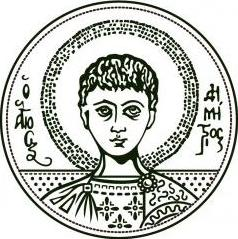
\includegraphics[width=\textwidth]{./figures/logo_apth}
        \end{flushleft}
    \end{minipage}
    \begin{minipage}{0.85\textwidth}
        \centering
        \text{\LARGE \ Αριστοτέλειο Πανεπιστήμιο Θεσσαλονίκης }\\\text{\Large Σχολή Θετικών Επιστημών }\\
        \text{\Large Τμήμα Μαθηματικών }\\
        \text{\large Θεωρητική Πληροφορική και Θεωρία Συστημάτων και Ελέγχου }
    \end{minipage}
    \vspace{8pt}
    \hrule
    \begin{center}
        \vspace{130pt}
        \text{\Large Εργασία για το μάθημα}\\
        \vspace{10pt}
        \rule{\textwidth}{1.5pt}
        \vspace{-30pt}
        \begin{center}
            \huge\bfseries{Κυρτή Βελτιστοποίηση}\par
        \end{center}
        \vspace{-10pt}
        \rule{\textwidth}{1.5pt}
        \vspace{25pt}
        \begin{minipage}{0.4\textwidth}
            \begin{center}
                \text{\large Νίκος Β. Βασίλας}
            \end{center}
        \end{minipage}
        \vspace{30pt}
        \vfill
        {\large \text{Θεσσαλονίκη, Ιανουάριος 2017}}
    \end{center}
\end{titlepage}

\clearemptypage

\titleformat{\chapter}[display]{\normalsize}{}
{}{ \bf\Huge }[\vspace{10pt}]

\tableofcontents
\clearemptypage

\listoffigures
\clearemptypage

\titleformat{\chapter}[display]{}{\titlerule[2.0pt]\vspace{5pt}\titlerule[0.5pt]\vspace{-8pt}
\LARGE{Κεφάλαιο} \bfseries\Huge\thechapter}
{10pt}{\titlerule[0.5pt] \vspace{20pt} \bf\huge }[\vspace{0pt}]

\chapter{Εισαγωγή}
Επιστήμονες από όλους τους κλάδους όπως μηχανικοί, μαθηματικοί, οικονομολόγοι
και άλλοι, έρχονται αντιμέτωποι με προβλήματα που πρέπει να λύσουν. Τα
προβλήματα πολλές φορές απαιτούν ένα βέλτιστο σχεδιασμό, όπως κατανομή σπάνιων πόρων,
σχεδιασμό βιομηχανικών δραστηριοτήτων, ή την εύρεση της τροχιάς ενός πυραύλου.
Στο παρελθόν, ένα μεγάλο εύρος λύσεων θεωρούταν αποδεκτό. Στον μηχανολογικό
σχεδιασμό για παράδειγμα, ήταν συνηθισμένη η χρήση μεγάλων παραγόντων ασφαλείας.
Όμως, λόγω του συνεχούς αυξανόμενου ανταγωνισμού, δεν είναι πλέον αρκετός
ο σχεδιασμός απλά αποδεκτών λύσεων. Σε άλλες περιπτώσεις, όπως για παράδειγμα ο
σχεδιασμός ενός διαστημικού οχήματος, οι αποδεκτές λύσεις είναι περιορισμένες.
Έτσι, γεννήθηκε η ανάγκη για απάντηση στα ερωτήματα όπως, αν κάνουμε αποδοτική
χρήση των σπάνιων πόρων, ή αν μπορούμε να κάνουμε ένα οικονομικότερο σχεδιασμό.
Ως απάντηση στο όλο και αυξανόμενο πεδίο τέτοιων ερωτήσεων, υπήρχε μία πολύ
γρήγορη ανάπτυξη μοντέλων και τεχνικών βελτιστοποίησης. Επίσης, η παράλληλη
ραγδαία εξέλιξη των υπολογιστικών δυνατοτήτων βοήθησε σημαντικά στη χρήση των
τεχνικών που αναπτύχθηκαν.

Η ιδέα της βελτιστοποίησης είναι βαθιά ριζωμένη ως η βασική αρχή στην ανάλυση
πολλών πολύπλοκων αποφάσεων. Χρησιμοποιώντας την ιδέα της βελτιστοποίησης,
προσεγγίζουμε ένα πολύπλοκο πρόβλημα, που περιλαμβάνει την επιλογή τιμών για
έναν αριθμό συγγενικών μεταβλητών, εστιάζοντας σε μία αντικειμενική συνάρτηση
που σχεδιάστηκε για να ποσοτικοποιήσει την επίδοση και να μετρήσει την ποιότητα
της απόφασης. Αυτή η αντικειμενική μεγιστοποιείται ή ελαχιστοποιείται και
υπόκειται σε περιορισμούς που ενδέχεται να περιορίσουν την επιλογή των
μεταβλητών απόφασης. Αν μία κατάλληλη πτυχή τους προβλήματος μπορεί να
απομονωθεί και να χαρακτηριστεί από μία αντικειμενική, είτε αυτό είναι κέρδος ή
ζημία στον επιχειρηματικό τομέα, είτε ταχύτητα ή απόσταση σε ένα φυσικό πρόβλημα
και τα λοιπά, η βελτιστοποίηση είναι το κατάλληλο εργαλείο για την ανάλυση των
προβλημάτων αυτών.

Είναι φυσικά εξαιρετικά σπάνια η περίπτωση όπου είναι εφικτό να περιγράψουμε
πλήρως όλες τις περίπλοκες αλληλεπιδράσεις των μεταβλητών, των περιορισμών και
να σχεδιάσουμε αντικειμενική συνάρτηση που αντιπροσωπεύει ένα πολύπλοκο
πρόβλημα απόφασης. Έτσι, η διατύπωση ενός προβλήματος βελτιστοποίησης μπορεί να
θεωρηθεί μόνο ως προσέγγιση του πραγματικού προβλήματος. Η ικανότητα στη
μοντελοποίηση, δηλαδή να συμπεριλάβουμε όλα τα σημαντικά στοιχεία ενός προβλήματος, και
η σωστή κρίση στην ερμηνεία των αποτελεσμάτων είναι απαραίτητα για την εξαγωγή
ορθών συμπερασμάτων. Η βελτιστοποίηση συνεπώς, πρέπει να θεωρείται ως ένα
εργαλείο για την καλύτερη κατανόηση και ανάλυση του προβλήματος.

Η ικανότητα και η ορθή κρίση, όσον αφορά τη διατύπωση του προβλήματος και την
ερμηνεία των αποτελεσμάτων, ενισχύεται μέσω της πρακτικής εμπειρίας και τη
μελέτη της θεωρίας. Η διατύπωση του προβλήματος πάντα περιλαμβάνει κάποιο
συμβιβασμό μεταξύ της αύξησης της μαθηματικής πολυπλοκότητας του προβλήματος και
την απόκλιση του μοντέλου από το πραγματικό πρόβλημα. Για να μπορέσει κάποιος να
επιλέξει τη χρυσή τομή πρέπει να είναι σε θέση να αναγνωρίσει την ιδιαιτερότητα
του κάθε προβλήματος, κάτι που είναι εφικτό μόνο με τη βαθιά μελέτη του τομέα.

Στην παρούσα εργασία παρουσιάζουμε κάποιους βασικούς τομείς της βελτιστοποίησης.
Σε κάθε κεφάλαιο αναλύουμε τη θεωρία που διέπει την κάθε κατηγορία προβλημάτων,
αναλύουμε κάποιον αλγόριθμο για την επίλυση του προβλήματος και δίνουμε κάποια
τυπικά παραδείγματα στο \tl{MATLAB}. Η εισαγωγή βασίστηκε ως επί τον πλείστον 
στα βιβλία \cite{bazaraa2013nonlinear} και \cite{luenberger2008linear}, και ο
ενδιαφερόμενος αναγνώστης παραπέμπεται εκεί για περαιτέρω πληροφορίες.

\clearemptypage

\chapter{Γραμμικός Προγραμματισμός}\label{ch:lp}
Ο στόχος του γραμμικού προγραμματισμού, σύμφωνα με~\cite{chong2010}, είναι να
προσδιορίσει τις τιμές των μεταβλητών που μεγιστοποιούν ή ελαχιστοποιούν μια γραμμική
αντικειμενική συνάρτηση, όπου οι μεταβλητές υπόκεινται σε κάποιους γραμμικούς περιορισμούς.
Το πρόβλημα του γραμμικού προγραμματισμού είναι μία ειδική κατηγορία ενός γενικού
προβλήματος βελτιστοποίησης με περιορισμούς. Στη γενική περίπτωση, ο στόχος είναι να βρούμε
ένα σημείο που ελαχιστοποιεί την αντικειμενική συνάρτηση και ταυτόχρονα ικανοποιεί τους περιορισμούς.
Οποιοδήποτε σημείο ικανοποιεί τους περιορισμούς ονομάζεται εφικτό σημείο. Στο πρόβλημα του γραμμικού
προγραμματισμού, η αντικειμενική συνάρτηση είναι γραμμική και το σύνολο των εφικτών σημείων καθορίζεται
από γραμμικές σχέσεις ισότητας και/ή ανισότητας.

Οι μέθοδοι για τη λύση προβλημάτων γραμμικού προγραμματισμού παρέχουν τη
δυνατότητα της επιλογής του καλύτερου εφικτού σημείου ανάμεσα στα πολλά εφικτά
σημεία. Γενικά, τα προβλήματα γραμμικού προγραμματισμού έχουν πολύ μεγάλο
μέγεθος, επομένως είναι απαραίτητοι αποδοτικοί μέθοδοι επίλυσης αυτών, που
πρωτοεμφανίστηκαν τέλη της δεκαετίας του 1930. Συγκεκριμένα το 1939, ο
\tl{Kantorovich}~\cite{kantorovich1939}, παρουσίασε διάφορες λύσεις σε
προβλήματα σχετικά με το σχεδιασμό παραγωγής και μεταφορών. Κατά τη διάρκεια του
Δεύτερου Παγκοσμίου Πολέμου, ο \tl{Koopmans}~\cite{koopmans1949} συνεισέφερε
σημαντικά στη λύση προβλημάτων μεταφοράς. Μάλιστα, και στους δύο προαναφερθέντες
απονεμήθηκε το Νόμπελ Οικονομίας το 1975 για τη συνεισφορά τους στη βέλτιστη κατανομή
πόρων. Το 1947, ο \tl{Dantzig}~\cite{dantzig1963} ανέπτυξε μία καινούργια μέθοδο λύσης
γραμμικών προγραμμάτων, γνωστή ως μέθοδος \tl{simplex}. Η μέθοδος αυτή είναι αποδοτική, παρέχει
μία κομψή λύση για το πρόβλημα και χρησιμοποιείται ευρέως ως και σήμερα για τα προβλήματα
του γραμμικού προγραμματισμού. Παρόλο αυτά, ο αριθμός των βημάτων, και ως εκ
τούτου ο συνολικός χρόνος, για την εύρεση λύσης αυξάνει εκθετικά με το μέγεθος των μεταβλητών.
Αυτό οδήγησε στο ενδιαφέρον για τη σχεδίαση αλγορίθμων που θα λύνουν γραμμικά προγράμματα με
πολυωνυμική πολυπλοκότητα, δηλαδή αλγόριθμοι που θα βρίσκουν τη βέλτιστη λύση σε χρόνο που θα
εξαρτάται πολυωνυμικά με τον αριθμό των μεταβλητών. Ο \tl{Khachiyan} το 1979
\cite{khachiyan1979}, ήταν ο πρώτος που ανέπτυξε έναν τέτοιο αλγόριθμο, ωστόσο έλαβε
περισσότερο θεωρητικό παρά πρακτικό ενδιαφέρον. Το 1984, ο \tl{Karmarkar}
\cite{karmarkar1984} πρότεινε ένα νέο αλγόριθμο γραμμικού προγραμματισμού με
πολυωνυμική πολυπλοκότητα, που φαίνεται να λύνει προβλήματα αρκετά πιο αποδοτικά
από ότι η μέθοδος \tl{simplex}. Η δουλεία του \tl{Karmarkar} οδήγησε σε άλλες μεθόδους,
που δε βασίζονται στη μέθοδο \tl{simplex}, γνωστές ως μέθοδοι εσωτερικού σημείου
(\tl{interior-point}).

Ένα τυπικό γραμμικό πρόγραμμα βελτιστοποίησης είναι της μορφής
\begin{equation}\label{eq:lp_min}
    \begin{aligned}
        & {\text{\tl{minimize}}}
        & & \vc{c}^T \vc{x} \\
        & \text{\tl{subject to}}
        & & \mt{A} \vc{x} = \vc{b} \\
        &&& \vc{x} \ge \vc{0},
    \end{aligned}
\end{equation}
όπου $\vc{c} \in \mathbb{R}^n$, $\vc{b} \in \mathbb{R}^m$, και
$\mt{A} \in \mathbb{R}^{m \times n}$. Ο περιορισμός ανισότητας $\vc{x} \ge \vc{0}$
για τις μεταβλητές σημαίνει ότι κάθε συνιστώσα του διανύσματος $\vc{x}$
είναι μη αρνητική. Πολλές παραλλαγές του παραπάνω προβλήματος είναι δυνατές,
όπως για παράδειγμα, αντί για ελαχιστοποίηση της αντικειμενικής συνάρτησης να ζητούμε
τη μεγιστοποίηση αυτής. Επίσης, οι περιορισμοί θα μπορούσαν αντί ισότητα, να είχαν
τη μορφή ανισότητας, όπως $\mt{A}\vc{x} \ge \vc{b}$, ή $\mt{A}\vc{x} \le \vc{b}$.
Αναφερόμαστε σε αυτές τις παραλλαγές ως γραμμικό πρόγραμμα, καθώς είναι δυνατόν να γραφτούν στην παραπάνω μορφή.

Κάθε γραμμικό πρόγραμμα ικανοποιεί έμμεσα κάποιες υποθέσεις, οι οποίες περιγράφονται
στο~\cite{hillier1985}. Η \textbf{αναλογικότητα} (\tl{proportionality}) αναφέρεται σε
ξεχωριστές δραστηριότητες, που εξετάζονται ανεξάρτητα από τις υπόλοιπες.
Ας υποθέσουμε ότι από τις $n$ δραστηριότητες μόνο μία υλοποιείται και
ας την ονομάσουμε $k$,  έτσι ώστε, $x_j = 0$, για $j = 1, \ldots, n$, εκτός
από $j = k$. Σύμφωνα με αυτή την υπόθεση το μέτρο αποτελεσματικότητας
είναι ίσο με $c_k x_k$ και η χρησιμοποίηση κάθε πόρου $i$ είναι ίση
με $a_{ik}x_k$. Αυτό σημαίνει ότι οι δύο ποσότητες είναι ευθέως ανάλογες
προς το επίπεδο της $k$ δραστηριότητας. Ακόμη σημαίνει ότι δεν υπάρχουν
αρχικές επιβαρύνσεις με την έναρξη της δραστηριότητας και ότι η αναλογικότητα
ισχύει για όλα τα επίπεδα τιμών της δραστηριότητας.

Με την υπόθεση της αναλογικότητας δεν εξασφαλίζεται ότι η αντικειμενική συνάρτηση
και οι περιορισμοί είναι γραμμικές συναρτήσεις. Η \textbf{προσθετικότητα}
(\tl{additivity}) προϋποθέτει ότι δεν υπάρχουν αλληλεπιδράσεις μεταξύ των
δραστηριοτήτων. Για κάθε επίπεδο δραστηριοτήτων $(x_1, \ldots, x_n)$ η
συνολική χρησιμοποίηση κάθε πόρου καθώς και το συνολικό μέτρο αποτελεσματικότητας
είναι ίσα με το άθροισμα των αντίστοιχων ποσοτήτων κάθε δραστηριότητας.

Μερικές φορές οι μεταβλητές αποφάσεων έχουν έννοια μόνο όταν παίρνουν
ακέραιες τιμές. Η λύση όμως που παίρνουμε από το γραμμικό προγραμματισμό
συχνά έχει μη ακέραιες τιμές. Με την υπόθεση της \textbf{διαιρετότητας}
(\tl{divisibility}) οι μονάδες δραστηριότητας μπορούν να διαιρεθούν σε
οποιοδήποτε κλασματικό επίπεδο, έτσι ώστε οι μη ακέραιες τιμές για τις μεταβλητές
αποφάσεων είναι επιτρεπτές.

\section{Επίλυση}
Στη συνέχεια θα παρουσιάσουμε κάποια παραδείγματα γραμμικού προγραμματισμού. Η
επίλυση αυτών έγινε με το λογισμικό \href{https://www.mathworks.com/products/matlab/}
{\tl{MATLAB}} και τη χρήση της βιβλιοθήκης βελτιστοποίησης (\tl{Optimization
Toolbox}) αυτού. Το \tl{MATLAB} δέχεται ένα γραμμικό πρόγραμμα στην παρακάτω μορφή
\begin{equation}\label{eq:lp_mat}
    \begin{aligned}
        & \underset{\vc{x}}{\text{\tl{minimize}}} & & \vc{f}^T \vc{x} \\
        & \text{\tl{subject to}} & & \mt{A} \vc{x} \leq \vc{b} \\
        &&& \mt{A}_{eq} \vc{x} = \vc{b}_{eq} \\
        &&& \vc{lb} \le \vc{x} \le \vc{ub}.
    \end{aligned}
\end{equation}
Στην παραπάνω σχέση, $\vc{f}$ είναι το διάνυσμα των συντελεστών της αντικειμενικής
συνάρτησης, $\mt{A}$ είναι το μητρώο των συντελεστών των ανισοτήτων και
$\vc{b}$ το αντίστοιχο διάνυσμα. Ακόμη, οι σχέσεις ισότητας περιγράφονται από το
μητρώο $\mt{A}_{eq}$ και το διάνυσμα $\vc{b}_{eq}$. Τέλος, $\vc{lb}$ και $\vc{ub}$ είναι
τα διανύσματα του κάτω και άνω ορίου του διανύσματος $\vc{x}$.

Η λύση γραμμικών προγραμμάτων γίνεται με τη συνάρτηση
\tl{\texttt{\textbf{linprog}}}. Η σύνταξή της είναι
\begin{otherlanguage}{english}
    \begin{center}
        \texttt{[x,fval,exitflag,output,lambda]=linprog(f,A,b,Aeq,beq,lb,ub,options)}
    \end{center}
\end{otherlanguage}
με απαραίτητα τα τρία πρώτα ορίσματα της συνάρτησης. Επιστρέφει τη βέλτιστη
λύση $\vc{x}$, την τιμή της αντικειμενικής συνάρτησης \tl{\texttt{fval}}, τη συνθήκη
εξόδου \tl{\texttt{exitflag}}, τη δομή (\tl{structure}) \tl{\texttt{output}}, σχετικά με
το τέλος του  προγράμματος και τους πολλαπλασιαστές \tl{Lagrange}
\tl{\texttt{lambda}}. Επίσης, από τη δομή \tl{\texttt{options}}, μπορούμε να ρυθμίσουμε
διάφορες παραμέτρους της διαδικασίας επίλυσης, όπως για παράδειγμα να επιλέξουμε
αλγόριθμο επίλυσης (\tl{interior-point, dual-simplex}), να θέσουμε ανοχές, δηλαδή το
κατά πόσο θα ικανοποιείται η αντικειμενική συνάρτηση, οι περιορισμοί, και άλλα πολλά.
Ο ενδιαφερόμενος παραπέμπεται στη βοήθεια του \tl{MATLAB}.

\subsection{Παράδειγμα 1}
Το πρώτο παράδειγμα προέρχεται από τη βοήθεια του \tl{MATLAB} και έχει
περιορισμούς ανισότητας, ισότητας καθώς και όρια στις μεταβλητές.
Η αντικειμενική συνάρτηση που θέλουμε να ελαχιστοποιήσουμε είναι
\begin{equation*}
    f(\vc{x}) = -x_1 - \frac{1}{3}x_2,
\end{equation*}
και οι σχέσεις ανισότητας που περιγράφουν το πρόβλημα είναι
\begin{align*}
    x_1 + x_2 &\leq 2 \\
    x_1 + \frac{1}{4}x_2 &\leq 1 \\
    x_1 - x_2 &\leq 2 \\
    -\frac{1}{4}x_1 - x_2 &\leq 1 \\
    -x_1 - x_2 &\leq -1 \\
    -x_1 + x_2 &\leq 2.
\end{align*}
Επίσης ισχύει ο περιορισμός ισότητας
\begin{equation*}
    x_1 + \frac{1}{4}x_2 = \frac{1}{2}
\end{equation*}
και τέλος έχουμε τα όρια
\begin{equation*}
    -1 \leq x_1 \leq 1.5, \qquad -0.5 \leq x_2 \leq 1.25.
\end{equation*}
Το παραπάνω πρόβλημα εύκολα γράφεται σε μητρωική μορφή και έτσι από τους περιορισμούς ανισότητας έχουμε
\begin{equation*}
    \mt{A} =
    \begin{bmatrix}
        1 & 1 \\
        1 & \frac{1}{4} \\
        1 & -1 \\
        -\frac{1}{4} & -1 \\
        -1 & -1 \\
        -1 & 1
    \end{bmatrix}, \qquad
    \vc{b} =
    \begin{bmatrix}
        2\\ 1\\ 2\\ 1\\ -1\\ 2
    \end{bmatrix}.
\end{equation*}
Ακόμη από τον περιορισμό ισότητας $\mt{A}_{eq} = \begin{bmatrix}1 & \frac{1}{4}\end{bmatrix}$,
$b_{eq} = \frac{1}{2}$, από τα κάτω και άνω όρια προκύπτει
$\vc{lb} = \begin{bmatrix}-1 & -0.5 \end{bmatrix}^T$, $\vc{ub} = \begin{bmatrix}1.5 & 1.25 \end{bmatrix}^T$
και τέλος από την αντικειμενική συνάρτηση έχουμε το διάνυσμα
$\vc{f} = \begin{bmatrix}-1 & -\frac{1}{3}\end{bmatrix}^T$. Λύνοντας το πρόβλημα,
βρίσκουμε ότι η βέλτιστη λύση είναι $\vc{x}^* = \begin{bmatrix} 0.1875 & -1.25 \end{bmatrix}^T$
και η αντίστοιχη τιμή της αντικειμενικής $f(\vc{x}^*) = -0.6042$. Παρακάτω παρατίθεται ο κώδικας
που χρησιμοποιήθηκε για να λυθεί το πρόβλημα.
\begin{otherlanguage}{english}
\lstinputlisting[language=Matlab]{src/lp1.m}
\end{otherlanguage}

\subsection{Παράδειγμα 2}
Το επόμενο παράδειγμα πρόκειται για πρόβλημα μεγιστοποίησης και καθότι πιο απλό,
είναι ιδιαίτερα χρήσιμο για να δούμε γεωμετρικά τη λύση του γραμμικού προγράμματος.
Το πρόβλημα είναι το εξής,
\begin{equation*}
    \begin{aligned}
        & \underset{\vc{x}}{\text{\tl{maximize}}} & & 4x + 3y \\
        & \text{\tl{subject to}} & & 2y \leq 25 - x \\
        &&& 4y \geq 2x - 8 \\
        &&& y \leq 2x - 5 \\
        &&& x \geq 0 \\
        &&& y \geq 2,
    \end{aligned}
\end{equation*}
ή στην ισοδύναμη συμπαγή μορφή
\begin{equation*}
    \begin{aligned}
        & \underset{\vc{x}}{\text{\tl{minimize}}} & & \vc{f}^T\vc{x} \\
        & \text{\tl{subject to}} & & \vc{A}\vc{x} \leq \vc{b},
    \end{aligned}
\end{equation*}
όπου $\vc{x} = \begin{bmatrix} x & y\end{bmatrix}^T$, $\vc{f} = \begin{bmatrix}-4 & -3\end{bmatrix}^T$ και
\begin{equation*}
    \mt{A} =
    \begin{bmatrix}
        1 & 2 \\
        2 & -4 \\
        -2 & 1 \\
        -1 & 0 \\
        0 & -1
    \end{bmatrix}, \qquad
    \vc{b} =
    \begin{bmatrix}
        25\\ 8\\ -5\\ 0\\ -2
    \end{bmatrix}.
\end{equation*}
Είναι προφανές ότι ένα πρόβλημα μεγιστοποίησης είναι το αντίθετο από ένα πρόβλημα ελαχιστοποίησης,
για αυτό μπορούμε εύκολα να γράψουμε το γραμμικό πρόγραμμα σε μορφή που
αναγνωρίζει το \tl{MATLAB}. Λύνοντας το πρόβλημα, βρίσκουμε ότι η βέλτιστη λύση
είναι $\vc{x}^* = \begin{bmatrix} 14.5 & 5.25 \end{bmatrix}^T$ και η αντίστοιχη τιμή
της αντικειμενικής $f(\vc{x}^*) = 73.75$. Παρακάτω παρατίθεται ο κώδικας που
χρησιμοποιήθηκε για να λυθεί το πρόβλημα.
\begin{otherlanguage}{english}
\lstinputlisting[language=Matlab]{src/lp2.m}
\end{otherlanguage}
Παρακάτω παρουσιάζεται η γραφική λύση του γραμμικού προγράμματος.
\begin{figure}[h]
    \centering
    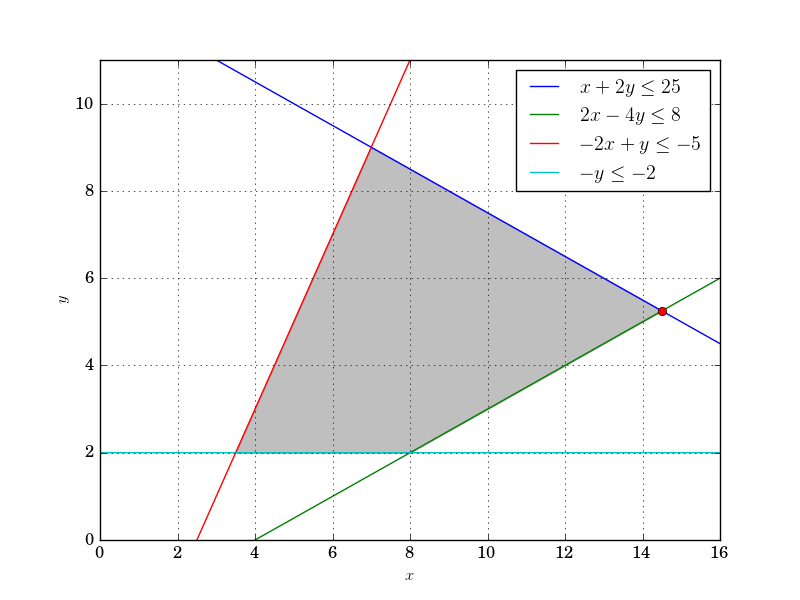
\includegraphics[width=\textwidth]{figures/lp2.png}
    \caption{Γραφική λύση του παραδείγματος 2
    του γραμμικού προγραμματισμού}\label{fig:lp2}
\end{figure}
Όπως φαίνεται από το σχήμα~\ref{fig:lp2} οι περιορισμοί του προβλήματος δημιουργούν
ένα πολύγωνο, γκρι σκιαγράφηση, όπου είναι ο χώρος των δυνατών λύσεων. Τελικά από όλα
τα σημεία του πολυγώνου το βέλτιστο φαίνεται στο σχήμα με την κόκκινη κουκκίδα και είναι
αυτό που μεγιστοποιεί την αντικειμενική συνάρτηση.

\subsection{Παράδειγμα 3}
Τα δεδομένα του επόμενου παραδείγματος προέρχονται από
\href{http://pythonhosted.org/PuLP/CaseStudies/a_blending_problem.html}{εδώ}.
Σύμφωνα με το παράδειγμα πρόκειται για ένα πραγματικό πρόβλημα γραμμικού προγραμματισμού.
Μία εταιρία που φτιάχνει τροφές για γάτες, επιδιώκει το χαμηλότερο δυνατό κόστος καθώς
και την επίτευξη των διατροφικών στόχων που έχουν τεθεί. Οι στόχοι αυτοί για τα $100 g$
προϊόντος, είναι τουλάχιστον $8 g$ πρωτεΐνης και $6 g$ λιπαρών, αλλά όχι παραπάνω
από $2 g$ φυτικών ινών και $0.4 g$ αλατιού. Επιδιώκουν δηλαδή να βρουν τη σωστή
αναλογία των βασικών συστατικών που μπορούν να χρησιμοποιήσουν (τα βασικά συστατικά
είναι κοτόπουλο, βοδινό, αρνί, ρύζι, σιτάρι και τζελ), ούτως ώστε να ικανοποιηθούν
οι στόχοι που αναφέραμε. Τα κόστη ανά γραμμάριο του κοτόπουλου, του βοδινού και του
αρνιού είναι $0.013\$, 0.008\$$ και $0.01\$$ αντίστοιχα, ενώ του ρυζιού, του
σιταριού και του τζελ $0.002\$, 0.005\$$ και $0.001\$$ αντίστοιχα. Κάθε βασικό
συστατικό συνεισφέρει στο συνολικό βάρος πρωτεΐνης, λιπαρών, φυτικών ινών και αλατιού
στο τελικό προϊόν. Η συνεισφορά του καθενός (σε γραμμάρια) ανά γραμμάριο συστατικού
παρουσιάζονται στο παρακάτω πίνακα.
\begin{table}[h]
    \centering
    \begin{tabulary}{0.95\textwidth}{| p{2cm} | C | C | C | C |}
        \hline
        {}        & Πρωτεΐνη & Λιπαρά & Φυτικές Ίνες & Αλάτι \\ \hline
        Κοτόπουλο      & $0.1$             & $0.08$                    & $0.001$                   & $0.002$ \\ \hline
        Χοιρινό      & $0.2$            & $0.1$                    & $0.005$                 & $0.005$ \\ \hline
        Αρνί      & $0.15$            & $0.11$                    & $0.003$                 & $0.007$ \\ \hline
        Ρύζι      & $0$             & $0.01$                    & $0.1$                  & $0.002$ \\ \hline
        Σιτάρι      & $0.04$            & $0.01$                    & $0.15$                 & $0.008$  \\ \hline
        Τζελ     & $0$             & $0$                    & $0$                  & $0$ \\ \hline
    \end{tabulary}
    \caption{Πίνακας Συστατικών}\label{table:lp3}
\end{table}
Αρχικά θα ορίσουμε ως μεταβλητές, το ποσοστό των συστατικών που μπορεί να
περιέχεται στη συσκευασία. Επειδή η συσκευασία είναι $100g$, τα ποσοστά
αυτά αντιπροσωπεύουν την ποσότητα των γραμμαρίων του κάθε συστατικού.
Ορίζουμε ως $x_1$ το ποσοστό του κοτόπουλου που περιέχεται στη
συσκευασία, $x_2$ το αντίστοιχο ποσοστό βοδινού, $x_3$ το ποσοστό
αρνιού, $x_4$ ρυζιού, $x_5$ φυτικών ινών και $x_6$ το ποσοστό
του τζελ. Στόχος είναι η μείωση του κόστους, και ορίζουμε ως
αντικειμενική συνάρτηση προς ελαχιστοποίηση
\begin{equation*}
    0.013x_1 + 0.008x_2 + 0.01x_3 + 0.002x_4 + 0.005x_5 + 0.001x_6,
\end{equation*}
σε δολάρια. Οι περιορισμοί του προβλήματος, έχουν περιγραφεί
παραπάνω και μπορούν να γραφτούν
\begin{align*}
    0.1x_1 + 0.2x_2 + 0.15x_3 + 0.04x_5 &\geq 8 \\
    0.08x_1 + 0.1x_2 + 0.11x_3 + 0.01x_4 + 0.01x_5 &\geq 6 \\
    0.001x_1 + 0.005x_2 + 0.003x_3 + 0.1x_4 + 0.15x_5 &\leq 2 \\
    0.002x_1 + 0.005x_2 + 0.007x_3 + 0.002x_4 + 0.008x_5 &\leq 2.
\end{align*}
Επίσης, έχουμε έναν προφανή περιορισμό ισότητας, ότι το
άθροισμα των συστατικών πρέπει να ισούται με όλη τη συσκευασία, δηλαδή
\begin{equation*}
    x_1 + x_2 + x_3 + x_4 + x_5 + x_6 = 100.
\end{equation*}
Τέλος, για κάθε ένα συστατικό $i$, έχουμε ένα κάτω και ένα
άνω όριο όπως φαίνεται στην παρακάτω σχέση
\begin{equation*}
    0 \leq x_i \leq 100.
\end{equation*}
Το παραπάνω πρόβλημα εύκολα γράφεται σε μητρωική μορφή και
έτσι από τους περιορισμούς ανισότητας έχουμε
\begin{equation*}
    \mt{A} =
    \begin{bmatrix}
        -0.1 & -0.2 & -0.15 & 0 & -0.04 & 0\\
        -0.08 & -0.1 & -0.11 & -0.01 & -0.01 & 0\\
        0.001 & 0.005 & 0.003 & 0.1 & 0.15 & 0\\
        0.002 & 0.005 & 0.007 & 0.002 & 0.008 & 0
    \end{bmatrix}, \qquad
    \vc{b} =
    \begin{bmatrix}
        -8\\ -6\\ 2\\ 0.4
    \end{bmatrix}.
\end{equation*}
Ακόμη από τον περιορισμό ισότητας $\mt{A}_{eq} = \begin{bmatrix}1 & 1 & 1 & 1 & 1 & 1\end{bmatrix}$,
$b_{eq} = 100$, από τα κάτω και άνω όρια προκύπτει
$\vc{lb} = \vc{0}_{6\times 1}^T$, $\vc{ub} = 100\vc{I}_{6 \times 1}^T$
και τέλος από την αντικειμενική συνάρτηση έχουμε το διάνυσμα
$\vc{f} = \begin{bmatrix}0.013 & 0.008 & 0.01 & 0.002 & 0.005 & 0.001\end{bmatrix}^T$.
Λύνοντας το πρόβλημα, βρίσκουμε ότι η βέλτιστη λύση είναι
$\vc{x}^* = \begin{bmatrix} 0 & 60 & 0 & 0 & 0 & 40\end{bmatrix}^T$,
δηλαδή $60\%$ βοδινό κρέας και $40\%$ τζελ, και η αντίστοιχη τιμή της
αντικειμενικής $f(\vc{x}^*) = 0.52$ δολάρια ανά συσκευασία.
Παρακάτω παρατίθεται ο κώδικας που χρησιμοποιήθηκε για να λυθεί το πρόβλημα.
\begin{otherlanguage}{english}
\lstinputlisting[language=Matlab]{src/lp3.m}
\end{otherlanguage}

\clearemptypage

\chapter{Τετραγωνικός Προγραμματισμός}\label{ch:qp}
Μία ειδική κατηγορία μη-γραμμικού προγραμματισμού παρουσιάζεται όταν η
αντικειμενική συνάρτηση $f$ είναι τετραγωνική και οι περιορισμοί είναι
γραμμικοί. Τότε το πρόβλημα ονομάζεται \textbf{Τετραγωνικός Προγραμματισμός} και
είναι της μορφής
\begin{equation}\label{eq:qp_min}
    \begin{aligned}
        & \underset{x}{\text{\tl{min}}}
        & & q(x) = \frac{1}{2}x^TGx + x^Tc \\
        & \text{\tl{subject to}}
        & & a^T_ix = b_i, \quad i \in \mathcal{E}, \\
        &&& a_i^Tx \ge b_i, \quad i \in \mathcal{I},
    \end{aligned}
\end{equation}
όπου $G$ είναι $n \times n$ συμμετρικό μητρώο, $\mathcal{E}$ και $\mathcal{I}$
είναι πεπερασμένα σύνολα των δεικτών, και $c, x,$ και $\{a_i\}, i \in
\mathcal{E}\cup \mathcal{I}$, είναι διανύσματα στο $\mathbb{R}^n$. Τετραγωνικά
προγράμματα μπορούν να λυθούν αριθμητικά (αν έχουν λύση) και η δυσκολία να
βρεθεί λύση εξαρτάται από τα χαρακτηριστικά της αντικειμενικής συνάρτησης και
τον αριθμό των περιορισμών. Έχουν αναπτυχθεί πολλές μέθοδοι επίλυσης προβλημάτων
τετραγωνικού προγραμματισμού που περιέχουν περιορισμούς ισότητας και ανισότητας.
Οι μέθοδοι ενεργών περιορισμών (\tl{active set}) χρησιμοποιούνται ευρέως από το
$1970$ και είναι αποτελεσματικοί για μικρό και μεσαίου μεγέθους προβλήματα.
Επιτρέπουν αποτελεσματική ανίχνευση της μη φραγμένης λύσης και τη μη εφικτότητας
και γενικά επιστρέφουν μία ακριβή εκτίμηση της βέλτιστης λύσης. Οι μέθοδοι
εσωτερικού σημείου (\tl{interior point}) είναι πιο πρόσφατοι και έγιναν
ιδιαιτέρως διάσημοι από το $1990$ και μετά. Είναι κατάλληλοι για μεγάλου
μεγέθους προβλήματα αλλά μπορεί να μην είναι οι πιο αποδοτικοί όταν θέλουμε να
λύσουμε παρόμοια τετραγωνικά προγράμματα, ο ενδιαφερόμενος αναγνώστης παραπέμπεται στο
\cite{boyd2004convex}. Μία άλλη μέθοδος είναι η προβολή
κλίσης (\tl{gradient projection}) και πρόκειται για ειδική περίπτωση της
μεθόδου των ενεργών περιορισμών, που είναι περισσότερο αποδοτική όταν οι μόνοι
περιορισμοί είναι τα όρια στις μεταβλητές. Στην παρούσα εργασία θα παρουσιάσουμε την
μέθοδο των ενεργών περιορισμών σύμφωνα με τη βοήθεια του
\cite{nocedal2006numerical}.

\section{Τετραγωνικό πρόγραμμα με περιορισμούς ισότητας}\label{sec:qp_eq}
Ξεκινάμε αναφέροντας την ειδική περίπτωση του γενικού προβλήματος
\eqref{eq:qp_min}, καθώς πολλοί αλγόριθμοι λύνουν σε κάθε
επανάληψη ένα υποπρόγραμμα με περιορισμούς ισότητας. Το τετραγωνικό πρόγραμμα
μπορεί να γραφτεί σε μητρωική μορφή
\begin{equation}\label{eq:qp_min_eq}
    \begin{aligned}
        & \underset{x}{\text{\tl{min}}}
        & & q(x) := \frac{1}{2}x^TGx + x^Tc \\
        & \text{\tl{subject to}}
        & & Ax = b,
    \end{aligned}
\end{equation}
όπου $A$ είναι η $m\times n$ Ιακωβιανή των περιορισμών με γραμμές τα $a_i^T, i
\in \mathcal{E}$ και $b$ είναι διάνυσμα στο $\mathbb{R}^m$ με συνιστώσες τα
$b_i, i \in \mathcal{E}$.

Οι πρώτης τάξης αναγκαίες συνθήκες για να είναι το $x^*$ λύση του
\eqref{eq:qp_min_eq} τότε υπάρχει διάνυσμα $\lambda^*$ τέτοιο ώστε να
ικανοποιείται το σύστημα
\begin{equation*}
    \begin{pmatrix}
        G & -A^T \\
        A & 0
    \end{pmatrix}
    \begin{pmatrix}
        x^* \\
        \lambda^*
    \end{pmatrix}=
    \begin{pmatrix}
        -c \\
        b
    \end{pmatrix}.
\end{equation*}
Το διάνυσμα $\lambda^*$ ονομάζονται πολλαπλασιαστές \tl{Lagrange}. Το παραπάνω
σύστημα μπορεί να γραφτεί σε μορφή βολική για τον υπολογισμό εκφράζοντας το
$x^*$ ως $x^* = x + p$, όπου $x$ είναι μία εκτίμηση της λύσης και $p$ είναι το
επιθυμητό βήμα. Με αυτόν το συμβολισμό προκύπτει
\begin{equation}\label{eq:qp_kkt}
    \begin{pmatrix}
        G & -A^T \\
        A & 0
    \end{pmatrix}
    \begin{pmatrix}
        -p \\
        \lambda^*
    \end{pmatrix}=
    \begin{pmatrix}
        g \\
        h
    \end{pmatrix},
\end{equation}
όπου
\begin{equation*}
    h Ax - b, \quad g = c + Gx, \quad p= x^* - x.
\end{equation*}
Το μητρώο στη \eqref{eq:qp_kkt} ονομάζεται \tl{Karush-Kuhn-Tucker (KKT)} μητρώο. Όταν
το μητρώο αυτό είναι μη ιδιάζων, τότε υπάρχει μοναδικό ζεύγος
$(x^*, \lambda^*)$ που ικανοποιεί της πρώτης τάξης αναγκαίες συνθήκες της
\eqref{eq:qp_min_eq}. Το \eqref{eq:qp_kkt} είναι σύστημα γραμμικών εξισώσεων και
έχουν αναπτυχθεί πολλές μέθοδοι για την αποτελεσματική επίλυσή του. Μερικές τις
άμεσες μεθόδους είναι η συμμετρική παραγοντοποίηση, η \tl{range-space} μέθοδος,
η \tl{null-space} μέθοδος. Κάποιες από τις έμμεσες μεθόδους, δηλαδή
επαναληπτικά, είναι οι \tl{Krylov} μέθοδοι, οι επαναληπτικοί μετασχηματισμοί
\tl{range-space} και οι επαναληπτικοί μετασχηματισμοί \tl{null-space}.

\section{Συνθήκες βέλτιστης λύσης}
Μπορούμε να ορίσουμε τη Λαγκρανζιανή για το πρόβλημα \eqref{eq:qp_min}
\begin{equation*}
    \mathcal{L}(x, \lambda) = \frac{1}{2}x^TGx + x^Tc - \sum_{i\in
    \mathcal{I}\cup \mathcal{E}}\lambda_i(a_i^Tx - b_i).
\end{equation*}
Το ενεργό σύνολο $\mathcal{A}(x^*)$ αποτελείται από όλους τους δείκτες των
περιορισμών για τους οποίους ισχύει η ισότητα στο $x^*$:
\begin{equation*}
    \mathcal{A}(x^*) = \{ i \in \mathcal{E}\cup \mathcal{I} \mid a^T_Ix^* =
    b_i\}.
\end{equation*}
Οι συνθήκες βέλτιστης λύσης \tl{Karush-Kuhn-Tucker conditions, (KKT conditions)}
\eqref{eq:qp_kkt_1}-\eqref{eq:qp_kkt_5} είναι
\begin{align}
    \nabla_x \mathcal{L}(x^*, \lambda^*) &= 0 \label{eq:qp_kkt_1} \\
    c_i(x^*) &= 0,\quad \tl{for all } i \in \mathcal{E}\label{eq:qp_kkt_2} \\
    c_i(x^*) &\geq 0,\quad \tl{for all } i \in \mathcal{I} \label{eq:qp_kkt_3}\\
    \lambda_i^* &\geq 0,\quad \tl{for all } i \in \mathcal{I} \label{eq:qp_kkt_4}\\
    \lambda_i^*c_i(x^*) &= 0,\quad \tl{for all } i \in \mathcal{E}\cup\mathcal{I}.\label{eq:qp_kkt_5}
\end{align}
Η σχέση \eqref{eq:qp_kkt_1} είναι γνωστή ως συνθήκη στασιμότητας
(\tl{stationarity condition}), οι σχέσεις \eqref{eq:qp_kkt_2} και
\eqref{eq:qp_kkt_3} ως συνθήκες εφικτότητας (\tl{primal feasibility})
με την υπόθεση ότι οι παράγωγοι των ενεργών περιορισμών ανισότητας και
ισότητας είναι γραμμικώς ανεξάρτητοι στο σημείο βέλτιστης λύσης (\tl{LICQ}),
η \eqref{eq:qp_kkt_4} ως συνθήκη μη-αρνητικότητας (\tl{dual feasibility})
και η \eqref{eq:qp_kkt_5} ως συνθήκη συμπληρωματικής χαλαρότητας
(\tl{complementary slackness}) και δηλώνει ότι είτε περιορισμό $i$ είναι ενεργός
είτε το αντίστοιχο $\lambda_i^* = 0$.

Αν γράψουμε τις συνθήκες \tl{KKT} για το πρόβλημα, τότε κάθε λύση της
\eqref{eq:qp_min} ικανοποιεί τις παρακάτω πρώτης τάξης συνθήκες βελτίστου, για
κάποιους πολλαπλασιαστές \tl{Lagrange} $\lambda^*_i, i \in \mathcal{A}(x^*)$:
\begin{align}
    Gx^* + c - \sum_{i\in \mathcal{I}\cup \mathcal{E}}\lambda_ia_i &=0
    \label{eq:qp_kktn_1}\\
    a_i^Tx^* &= b_i,\quad \tl{for all } i \in \mathcal{A}(x^*)
    \label{eq:qp_kktn_2}\\
    a_i^Tx^* &\geq b_i,\quad \tl{for all } i \in
    \mathcal{I}\setminus\mathcal{A}(x^*) \label{eq:qp_kktn_3}\\
    \lambda_i^* &\geq 0,\quad \tl{for all } i \in
    \mathcal{I}\cap\mathcal{A}(X^*).\label{eq:qp_kktn_4}
\end{align}

\section{Μέθοδος ενεργών περιορισμών}
Η μέθοδος των ενεργών περιορισμών για τα τετραγωνικά προγράμματα παρουσιάζει τις
παραλλαγές: \tl{primal, dual, primal-dual}. Θα περιγράψουμε την πρώτη κατηγορία,
η οποία μέσω επαναλήψεων βρίσκει εφικτές λύσεις του \eqref{eq:qp_min} ενώ παράλληλα μειώνει την
αντικειμενική συνάρτηση $q(x)$.

Η μέθοδος βρίσκει ένα βήμα από τη μία επανάληψη στην άλλη λύνοντας ένα
τετραγωνικό υπό πρόβλημα όπου κάποιοι περιορισμοί ανισότητας και οι περιορισμοί
ισότητας αντιμετωπίζονται ως ισότητες. Το υποσύνολο αυτό ονομάζεται σύνολο
εργασίας (\tl{working set}) και συμβολίζεται στην $k$ επανάληψη $x_k$ με $\mathcal{W}_k$. Μία
σημαντική απαίτηση είναι τα $a_i$ των περιορισμών να είναι γραμμικώς ανεξάρτητα.

Δοθέντας επανάληψης $x_k$ και συνόλου εργασίας $\mathcal{W}_k$, αρχικά ελέγχουμε
αν το $x_k$ ελαχιστοποιεί τη τετραγωνική $q$ στον υποχώρο που ορίζει το σύνολο
εργασίας. Αν όχι, υπολογίζουμε βήμα $p$ λύνοντας τετραγωνικό υποπρόγραμμα όπου
οι περιορισμοί που αντιστοιχούν στο σύνολο $\mathcal{W}_k$ θεωρούνται ισότητες
και οι υπόλοιποι περιορισμοί δε λαμβάνονται προσωρινά υπόψιν. Για να εκφράσουμε
το υποπρόβλημα ως προς το βήμα $p$, ορίζουμε
\begin{equation*}
    p = x - x_k, \quad g_k= Gx_k + c.
\end{equation*}
Με αντικατάσταση του $x$ στην αντικειμενική συνάρτηση βρίσκουμε
\begin{equation*}
    q(x) = q(x_k + p) = \frac{1}{2}p^TGp + g_k^Tp + \rho_k,
\end{equation*}
όπου $\rho_k = \frac{1}{2} x^T_kGx_k + c^Tx_k$ είναι ανεξάρτητο του $p$. Έτσι
μπορούμε να αγνοήσουμε το $\rho_k$ χωρίς να αλλάξει η λύση του προβλήματος και
έτσι το τετραγωνικό πρόγραμμα για να λυθεί στην $k$ επανάληψη είναι
\begin{equation}\label{eq:qp_min_sub}
    \begin{aligned}
        & \underset{p}{\text{\tl{min}}}
        & & \frac{1}{2}p^TGp + g^T_kp \\
        & \text{\tl{subject to}}
        & & a^T_ip = 0, \quad i \in \mathcal{W}_k.
    \end{aligned}
\end{equation}
Συμβολίζουμε τη λύση του παραπάνω υποπρογράμματος με $p_k$. Παρατηρούμε ότι για
κάθε $i \in \mathcal{W}_k$, η τιμή του $a_i^Tx$ δεν μεταβάλλεται καθώς
κινούμαστε στο $p_k$, αφού $a_i^T(x_k + \alpha p_k) = a_i^T = b_i$ για κάθε
$\alpha$. Αφού οι περιορισμοί στο $\mathcal{W}_k$ ικανοποιούνται στο $x_k$, θα
ικανοποιούνται και στο $x_k + \alpha p_k$, για κάθε $\alpha$. Η λύση του
\eqref{eq:qp_min_sub} μπορεί να υπολογισθεί με κάποια από τις τεχνικές που
αναφέρθηκαν στο κεφάλαιο~\ref{sec:qp_eq}.

Έστω ότι η βέλτιστη λύση $p_k$ του \eqref{eq:qp_min_sub} είναι μη μηδενική, τότε
πρέπει να αποφασίσουμε πόσο μακριά να κινηθούμε σε αυτή τη διεύθυνση. Αν
$x_k + p_k$ είναι εφικτό ως προς όλους τους περιορισμούς, τότε θέτουμε
$x_{k+1} = x_k + p_k$. Διαφορετικά θέτουμε
\begin{equation*}
    x_{k+1} = x_k + \alpha_k p_k,
\end{equation*}
όπου το μήκος βήματος $\alpha_k$ επιλέγεται να είναι η μεγαλύτερη δυνατή τιμή του
διαστήματος $[0,1]$ για το οποίο ικανοποιούνται όλοι οι περιορισμοί. Μπορούμε να
βρούμε έναν ορισμό για το $\alpha_k$ αν εξετάσουμε πως επηρεάζει τους
περιορισμούς $i \not\in \mathcal{W}_k$, καθώς οι περιορισμοί $i \in
\mathcal{W}_k$ θα ικανοποιούνται ανεξαρτήτως της επιλογής του $\alpha_k$. Αν
$a_i^Tp_k \geq 0$ για κάποιο $i \not\in \mathcal{W}_k$, τότε για όλα τα
$\alpha_k \geq 0$ έχουμε $a_i^T(x_k + \alpha_k p_k) \geq a_i^Tx_k \geq b_i$.
Έτσι, ο περιορισμός $i$ θα ικανοποιείται για όλες τις μη αρνητικές τιμές του
μήκους βήματος. Όταν $a_i^T p_k < 0$ για κάποιο $i \not\in \mathcal{W}_k$,
έχουμε $a_i^T(x_k + \alpha_k p_k) \geq b_i$ μόνο όταν
\begin{equation*}
    \alpha_k \leq \dfrac{b_i - a_i^Tx_k}{a_i^Tp_k}.
\end{equation*}
Για να μεγιστοποιήσουμε τη μείωση στη $q$, θέλουμε το $\alpha_k$ να είναι όσο το
δυνατόν μεγαλύτερο στο $[0,1]$ υπό τον περιορισμό να διατηρεί την εφικτότητα,
έτσι έχουμε τον παρακάτω ορισμό
\begin{equation}\label{eq:qp_step_l}
    \alpha_k := \min\left( 1,\min_{i \not\in \mathcal{W}_k, a^T_ip_k <
    0}\dfrac{b_i - a^T_i x_k}{a_i^Tp_k} \right).
\end{equation}
Ονομάζουμε τους περιορισμούς $i$ για τους οποίους το ελάχιστο στη
\eqref{eq:qp_step_l} ικανοποιείται περιορισμούς παρεμπόδισης (\tl{blocking
constraints}). Αν $\alpha_k = 1$ και κανένας νέος περιορισμός είναι ενεργός στο $x_k
+ \alpha_k p_k$, τότε δεν υπάρχουν καθόλου περιορισμοί παρεμπόδισης. Παρατηρούμε
ότι είναι εφικτό το $\alpha_k$ να είναι μηδέν, γιατί θα μπορούσαμε να είχαμε
$a_i^Tp_k < 0$ για κάποιον περιορισμό $i$ που είναι ενεργός στο $x_k$ αλλά να
μην ανήκει στο σύνολο εργασίας $\mathcal{W}_k$.

Αν $\alpha_k < 1$, τότε το βήμα κατά μήκος του $p_k$ παρεμποδίζεται από κάποιον
περιορισμό που δεν ανήκει στο $\mathcal{W}_k$ και δημιουργείται νέο σύνολο
εργασίας $\mathcal{W}_{k+1}$ λαμβάνοντας υπόψιν τον περιορισμό αυτόν.

Συνεχίζουμε τις επαναλήψεις σύμφωνα με την παραπάνω λογική, προσθέτοντας
περιορισμούς στο σύνολο εργασίας μέχρι να βρούμε σημείο $\hat{x}$ που
ελαχιστοποιεί την τετραγωνική αντικειμενική συνάρτηση ως προς το τρέχων σύνολο
εργασίας $\mathcal{\hat{W}}$. Εύκολα αναγνωρίζουμε το σημείο αυτό, καθώς το
υποπρόβλημα \eqref{eq:qp_min_sub} έχει λύση $p = 0$. Εφόσον το $p = 0$
ικανοποιεί τις συνθήκες βέλτιστης λύσης \eqref{eq:qp_kkt} για το
\eqref{eq:qp_min_sub} ισχύει
\begin{equation}\label{eq:qp_1642}
    \sum_{i\in \mathcal{\hat{W}}} a_i \hat{\lambda}_i = g = G\hat{x} + c,
\end{equation}
για κάποιους πολλαπλασιαστές \tl{Lagrange} $\hat{\lambda}_i, i \in
\mathcal{\hat{W}}$. Τα $\hat{x}$ και $\hat{\lambda}$ ικανοποιούν την πρώτη
συνθήκη \tl{KKT} \eqref{eq:qp_kktn_1}, αν ορίσουμε τους πολλαπλασιαστές των
ανισοτήτων που δεν ανήκουν στο σύνολο εργασίας να είναι μηδέν. Εξαιτίας του
ελέγχου στο μήκος βήματος, το $\hat{x}$ είναι εφικτό ως προς όλους τους
περιορισμούς, έτσι οι σχέσεις \eqref{eq:qp_kktn_2} και \eqref{eq:qp_kktn_3}
ικανοποιούνται.

Αν οι πολλαπλασιαστές που αντιστοιχούν στους περιορισμούς ανισότητας του συνόλου
εργασίας, δηλαδή $i \in \mathcal{\hat{W}}\cap \mathcal{I}$, είναι μη αρνητικοί,
τότε η \eqref{eq:qp_kktn_4} ικανοποιείται και έτσι το $\hat{x}$ ικανοποιεί τις
συνθήκες βελτίστου και συνεπώς ικανοποιεί το αρχικό πρόβλημα
\eqref{eq:qp_min}.

Αν από την άλλη, κάποιος από τους περιορισμούς $\hat{\lambda_j}, j \in
\mathcal{\hat{W}}\cap \mathcal{I}$, είναι αρνητικός τότε η συνθήκη
\eqref{eq:qp_kktn_4} δεν ικανοποιείται και η αντικειμενική συνάρτηση μπορεί να
μειωθεί αν αφαιρέσουμε τον $j$ περιορισμό από το σύνολο εργασίας και λύσουμε ένα
νέο υποπρόβλημα για νέο βήμα. Με τον τρόπο αυτόν, δημιουργούμε μία διεύθυνση
$p$ στη νέα επανάληψη που είναι εφικτή ως προς τον περιορισμό που αφαιρέθηκε.

Στο σημείο αυτό έχουμε περιγράψει τα βασικά σημεία της μεθόδου ενεργών
περιορισμών. Παρακάτω παρουσιάζεται η μέθοδος σε μορφή αλγορίθμου για προβλήματα
κυρτού τετραγωνικού προγραμματισμού, όπου υποθέτουμε ότι η αντικειμενική
συνάρτηση $q$ είναι φραγμένη στο εφικτό σύνολο των περιορισμών της
\eqref{eq:qp_min}.
\begin{figure}[h]
    \begin{otherlanguage}{english}
        \begin{algorithmic}
            \REQUIRE \text{\gr{Δώσε αρχικό εφικτό σημείο }}$x_0;$
            \REQUIRE \text{\gr{Το αρχικό σύνολο }}$\mathcal{W}_0$\text{\gr{ να είναι υποσύνολο
            των ενεργών περιορισμών στο }}$x_0;$
            \FOR{$k=0,1,2,\dots$}
            \STATE \text{\gr{Λύσε }}\eqref{eq:qp_min_sub}\text{\gr{ και βρες
            }}$p_k;$
            \IF{$p_k=0$}
            \STATE \text{\gr{Βρες }}$\hat{\lambda}_i$\text{\gr{ που ικανοποιούν
            }}\eqref{eq:qp_1642}\text{\gr{ με }}$\mathcal{\hat{W}} =
            \mathcal{W}_k;$
            \IF{$\hat{\lambda_i} \geq 0$\text{\gr{ για όλα τα }}$i \in
            \mathcal{W}_k \cap \mathcal{I}$}
            \RETURN $x^* = x_k;$
            \ELSE
            \STATE $j \leftarrow
            \text{arg}\min_{j\in\mathcal{W}_k\cap\mathcal{I}}\hat{\lambda}_j;$
            \STATE $x_{k+1} \leftarrow x_k; \mathcal{W}_{k+1} \leftarrow
            \mathcal{W}_k\setminus{j};$
            \ENDIF
            \ELSE
            \STATE \text{\gr{υπολόγισε }}$\alpha_k$\text{\gr{ από
            }}\eqref{eq:qp_step_l}$;$
            \STATE $x_{k+1} \leftarrow x_k + \alpha_kp_k;$
            \IF{\text{\gr{υπάρχουν περιορισμοί παρεμπόδισης}}}
            \STATE \text{\gr{βρες }}$\mathcal{W}_{k+1}$\text{\gr{ προσθέτοντας
            τον περιορισμό παρεμπόδισης του }}$\mathcal{W}_k;$
            \ELSE
            \STATE $\mathcal{W}_{k+1} \leftarrow \mathcal{W}_k;$
            \ENDIF
            \ENDIF
            \ENDFOR
        \end{algorithmic}
    \end{otherlanguage}
    \caption{\gr{Αλγόριθμος ενεργών περιορισμών}}
\end{figure}

Όπως βλέπουμε από τον αλγόριθμο, απαιτείται ένα αρχικό εφικτό σημείο
για να ξεκινήσει. Διάφορες τεχνικές έχουν αναπτυχθεί για τον υπολογισμό αυτού.
Επιγραμματικά θα αναφέρουμε μία από αυτές. Αν $\tilde{x}$ είναι μία αρχική εκτίμηση του
διανύσματος $x$, η οποία μπορεί να μην είναι εφικτή, τότε μπορούμε να ορίσουμε το
ακόλουθο εφικτό γραμμικό πρόγραμμα
\begin{equation*}
    \begin{aligned}
        & \underset{(x,z)}{\text{\tl{min}}}
        & & e^Tz\\
        & \text{\tl{subject to}}
        & & a^T_ix + \gamma_iz_i = b_i, \quad i \in \mathcal{E}, \\
        &&& a_i^Tx + \gamma_iz_ \ge b_i, \quad i \in \mathcal{I}, \\
        &&& z \ge 0,
    \end{aligned}
\end{equation*}
όπου $e= \begin{pmatrix}1 & \dots & 1\end{pmatrix}^T, \gamma_i = -
\text{\tl{sign}}(a_i^T\tilde{x}-b_i)$ για $i \in \mathcal{E}$, και $\gamma_i =
1$ για $i \in \mathcal{I}$. Ένα εφικτό αρχικό σημείο για το πρόβλημα είναι
\begin{equation*}
    x = \tilde{x},\quad
    z_i = |a_i^T\tilde{x} - b_i|\ (i \in \mathcal{E}),\quad
    z_i = \max{b_i - a_i^T\tilde{x}, 0}\ (i \in \mathcal{I}).
\end{equation*}
Αποδεικνύεται ότι αν $\tilde{x}$ είναι εφικτό σημείο για το αρχικό πρόβλημα
\eqref{eq:qp_min} τότε το $(\tilde{x}, 0)$ είναι βέλτιστο για το εφικτό
υποπρόβλημα. Γενικά, αν το αρχικό τετραγωνικό πρόγραμμα έχει εφικτά σημεία,
τότε βέλτιστη αντικειμενική συνάρτηση του παραπάνω υποπροβλήματος είναι μηδέν,
και κάθε λύση του υποπροβλήματος δίνει εφικτό σημείο στο αρχικό πρόβλημα. Τέλος,
το αρχικό σύνολο εργασίας $\mathcal{W}_0$ μπορεί να βρεθεί παίρνοντας γραμμικώς
ανεξάρτητα υποσύνολα των ενεργών περιορισμών στη λύση του υποπροβλήματος.

\section{Επίλυση}
Θα παρουσιάσουμε ένα παράδειγμα τετραγωνικού προγραμματισμού με χρήση του
λογισμικού \href{https://www.mathworks.com/products/matlab/}{\tl{MATLAB}}
και τη χρήση της βιβλιοθήκης βελτιστοποίησης (\tl{Optimization Toolbox}) αυτού.
Το \tl{MATLAB} δέχεται ένα τετραγωνικό πρόγραμμα στην παρακάτω μορφή
\begin{equation}\label{eq:qp_mat}
    \begin{aligned}
        & \underset{x}{\text{\tl{min}}} & &
        \dfrac{1}{2}x^THx + f^T x \\
        & \text{\tl{subject to}} & & Ax \leq b \\
        &&& A_{eq} x = b_{eq} \\
        &&& lb \le x \le ub.
    \end{aligned}
\end{equation}
Στην παραπάνω σχέση, $H$ είναι το μητρώο των τετραγωνικών όρων στην
αντικειμενική συνάρτηση, $f$ είναι το διάνυσμα των γραμμικών συντελεστών,
$A$ είναι το μητρώο των συντελεστών των ανισοτήτων και $b$ το
αντίστοιχο διάνυσμα. Ακόμη, οι σχέσεις ισότητας περιγράφονται από το
μητρώο $A_{eq}$ και το διάνυσμα $b_{eq}$. Τέλος, $lb$ και $ub$ είναι
τα διανύσματα του κάτω και άνω ορίου του διανύσματος $x$.

Η λύση τετραγωνικών προγραμμάτων γίνεται με τη συνάρτηση
\tl{\texttt{\textbf{quadprog}}}. Η σύνταξή της είναι
\begin{otherlanguage}{english}
    \begin{center}
        \texttt{[x,fval,exitflag,output,lambda]=quadprog(H,f,A,b,Aeq,beq,lb,ub,x0,options)}
    \end{center}
\end{otherlanguage}
με απαραίτητα τα δύο πρώτα ορίσματα της συνάρτησης. Επιστρέφει τη βέλτιστη
λύση $x$, την τιμή της αντικειμενικής συνάρτησης \tl{\texttt{fval}}, τη συνθήκη
εξόδου \tl{\texttt{exitflag}}, τη δομή (\tl{structure}) \tl{\texttt{output}}, σχετικά με
το τέλος του  προγράμματος και τους πολλαπλασιαστές \tl{Lagrange}
\tl{\texttt{lambda}}. Επίσης, από τη δομή \tl{\texttt{options}}, μπορούμε να ρυθμίσουμε
διάφορες παραμέτρους της διαδικασίας επίλυσης, όπως για παράδειγμα να επιλέξουμε
αλγόριθμο επίλυσης (\tl{interior-point-convex, trust-region-reflective}, ο
    πρώτος είναι για κυρτά τετραγωνικά και ο δεύτερος αλγόριθμος μπορεί να
χρησιμοποιηθεί όταν έχουμε μόνο όρια στις μεταβλητές ή και περιορισμούς ισότητας),
να θέσουμε ανοχές, δηλαδή το κατά πόσο θα ικανοποιείται η αντικειμενική συνάρτηση,
οι περιορισμοί, να δώσουμε μία αρχική λύση, και άλλα πολλά. Ο ενδιαφερόμενος
παραπέμπεται στη βοήθεια του \tl{MATLAB}.

\subsection{Παράδειγμα}
Το παράδειγμα προέρχεται από τη βοήθεια του \tl{MATLAB} και έχει
περιορισμούς ανισότητας, καθώς και όρια στις μεταβλητές.
Η αντικειμενική συνάρτηση που θέλουμε να ελαχιστοποιήσουμε είναι
\begin{equation*}
    f(x) = \frac{1}{2}x_1^2 + x_2^2 - x_1x_2 -2x_1 - 6x_2,
\end{equation*}
οι σχέσεις ανισότητας που περιγράφουν το πρόβλημα είναι
\begin{align*}
    x_1 + x_2 &\leq 2 \\
    -x_1 + 2x_2 &\leq 2 \\
    2x_1 + x_2 &\leq 3,
\end{align*}
και τέλος έχουμε τα όρια
\begin{equation*}
    0 \leq x_1, \qquad 0 \leq x_2.
\end{equation*}
Το παραπάνω πρόβλημα εύκολα γράφεται σε μητρωική μορφή
\begin{equation*}
    f(x) = \dfrac{1}{2}x^THx + f^Tx,
\end{equation*}
όπου
\begin{equation*}
    H = \begin{pmatrix}1 & -1 \\-1 & 2\end{pmatrix},\quad
    f = \begin{pmatrix}-2\\-6\end{pmatrix},\quad
    x = \begin{pmatrix}x_1\\x_2\end{pmatrix}.
\end{equation*}
Επίσης, το μητρώο των περιορισμών $A$ και το αντίστοιχο διάνυσμα $b$ είναι
\begin{equation*}
    A = \begin{pmatrix}1 & 1\\-1 & 2\\2 & 1\end{pmatrix},\quad
    b = \begin{pmatrix}2\\2\\3\end{pmatrix}.
\end{equation*}
Λύνοντας το πρόβλημα, βρίσκουμε ότι η βέλτιστη λύση είναι
$x^* = \begin{pmatrix} 0.667 & 1.333 \end{pmatrix}^T$ και η αντίστοιχη
τιμή της αντικειμενικής $f(x^*) = -8.2222$.

Στο σχήμα~\ref{fig:qp} παρουσιάζεται η γραφική λύση του προγράμματος. Σημειώνεται
με ροζ αστερίσκο επάνω στην καμπύλη το ελάχιστο του προβλήματος. Στη συνέχεια
παρατίθεται ο κώδικας του \tl{MATLAB} που χρησιμοποιήθηκε για να λυθεί το πρόβλημα.
\newpage
\begin{otherlanguage}{english}
    \begin{figure}[h!]
        \centering
        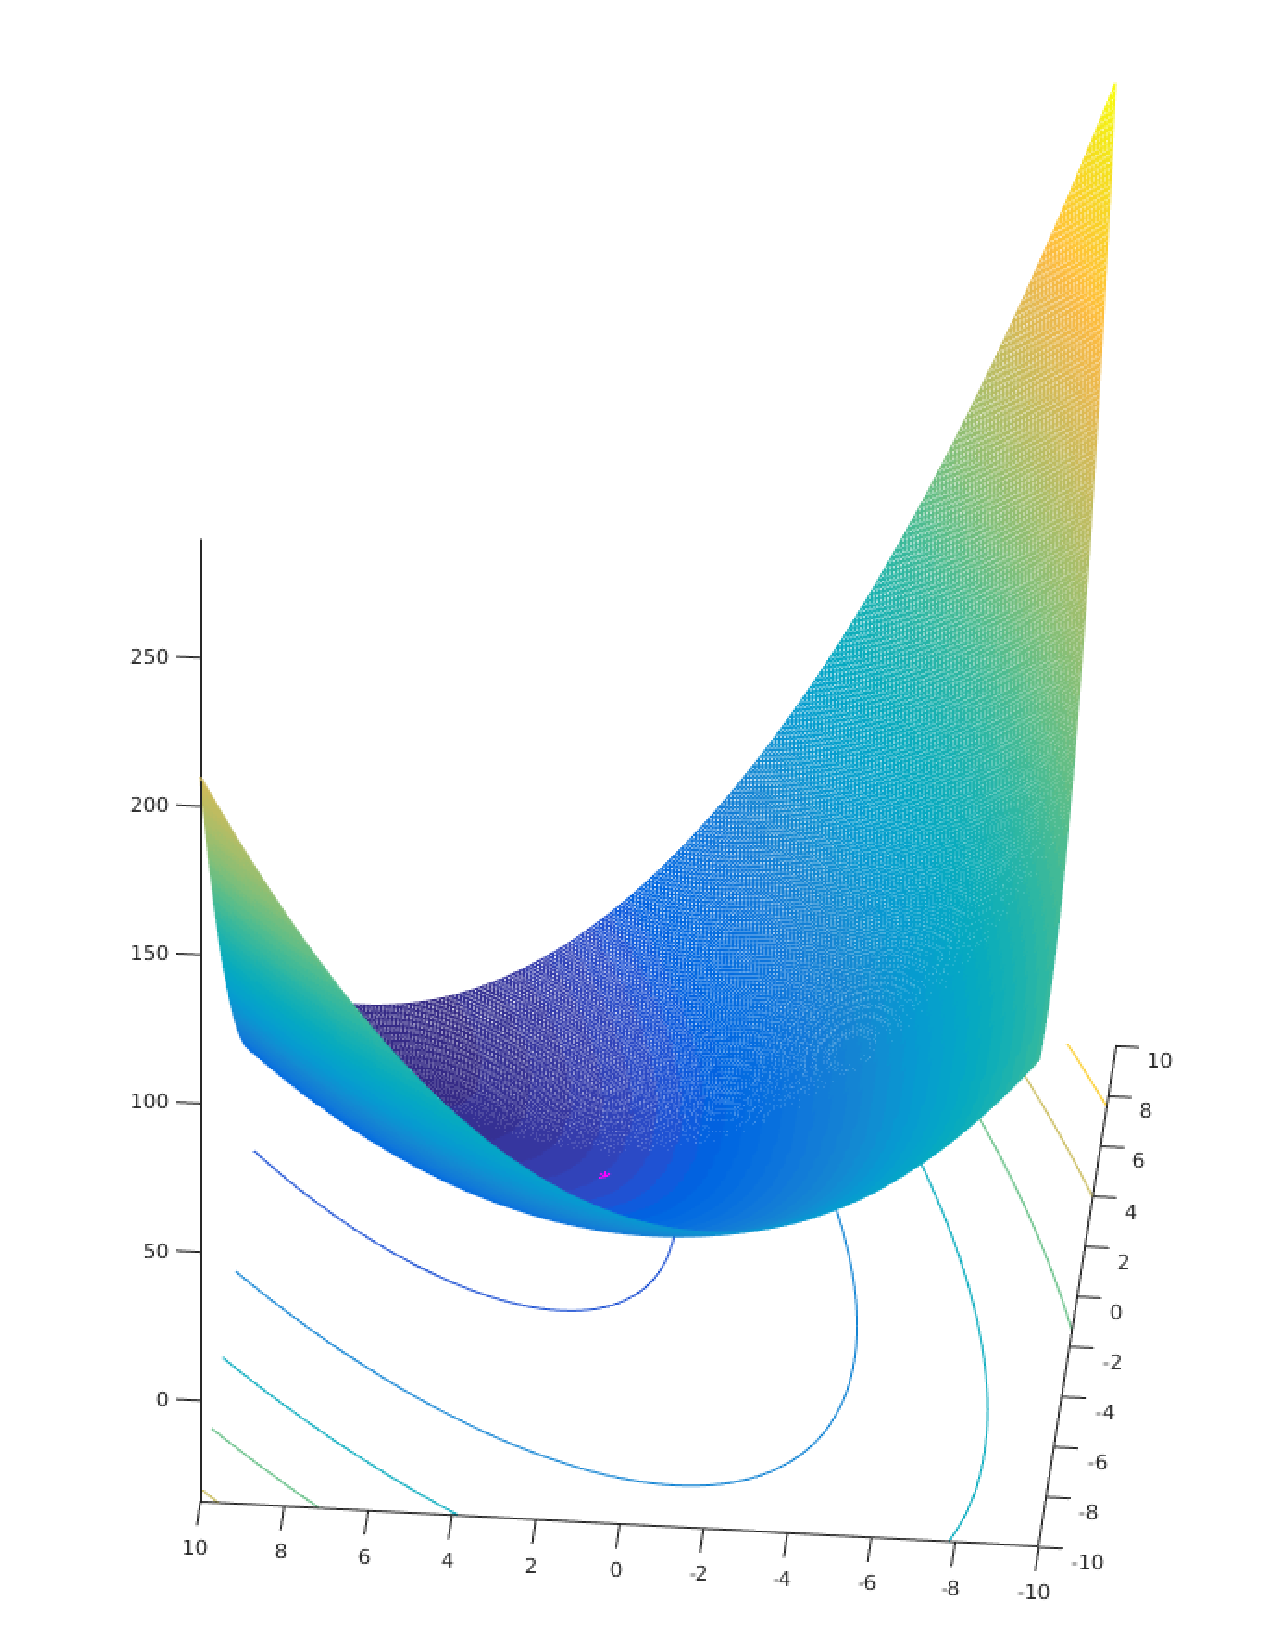
\includegraphics[width=\textwidth]{figures/qp.pdf}
        \caption{\gr{Λύση παραδείγματος του τετραγωνικού προγραμματισμού}}\label{fig:qp}
    \end{figure}
\end{otherlanguage}

\begin{otherlanguage}{english}
    \lstinputlisting[language=Matlab]{src/qp.m}
\end{otherlanguage}

\clearemptypage

\chapter{Κυρτά Σύνολα}
\section{Αφινικά και κυρτά σύνολα}
\subsection{Γραμμή και τμήμα γραμμής} Όλα τα σημεία που περιγράφονται από τη σχέση
\begin{equation*}
    x = \theta x_1 + (1 - \theta) x_2,
\end{equation*}
με $x_1, x_2 \in \mathbf{R}^n$ και $\theta \in \mathbf{R}$, αποτελούν μία
\textbf{γραμμή} που περνάει από τα $x_1, x_2$. Για $\theta = 0$ έχουμε $x = x_2$
ενώ $\theta  = 1$ αντιστοιχεί σε $x = x_1$. Τιμές της παραμέτρου $\theta$ στο
μεταξύ $0$ και $1$ δίνουν \textbf{τμήμα γραμμής} ανάμεσα στα $x_1$ και $x_2$.

\subsection{Αφινικό σύνολο} Ένα σύνολο $C \subseteq \mathbf{R}^n$ ονομάζεται \textbf{αφινικό} αν η γραμμή
μεταξύ δύο οποιοδήποτε διαφορετικών σημείων που ανήκουν στο $C$, βρίσκεται στο
$C$. Για παράδειγμα αν για οποιοδήποτε $x_1, x_2 \in C$ και $\theta \in
\mathbf{R}$ τότε
\begin{equation*}
    x = \theta x_1 + (1 - \theta) x_2 \in C.
\end{equation*}
Με άλλα λόγια, το σύνολο $C$ περιέχει το γραμμικό συνδυασμό δύο
σημείων, ο οποίος βρίσκεται στο $C$ δεδομένου ότι οι συντελεστές στο
γραμμικό συνδυασμό αθροίζονται στη μονάδα. Η ιδέα αυτή μπορεί να γενικευτεί για
παραπάνω από δύο σημεία. Το σημείο της μορφής $\theta_1 x_1 + \dots + \theta_k
x_k$, όπου $\theta_1 + \dots + \theta_k = 1$, αναφέρεται ως \textbf{αφινικός
συνδυασμός} των σημείων $x_1 + \dots + x_k$. Ένα χαρακτηριστικό παράδειγμα
αφινικού συνόλου είναι το σύστημα γραμμικών εξισώσεων της μορφής
$Ax = b$. Επίσης, ισχύει ότι κάθε αφινικό σύνολο μπορεί να
εκφραστεί ως ένα σύστημα γραμμικών εξισώσεων. Το σύνολο όλων των αφινικών
συνδυασμών των σημείων του συνόλου $C \subseteq \mathbf{R}^n$
ονομάζεται \textbf{αφινική θήκη} του $C$ και συμβολίζεται με
$\textbf{\tl{aff}} \ C$.

\begin{figure}
    \centering
    \begin{subfigure}[b]{.4\textwidth}
        \centering
        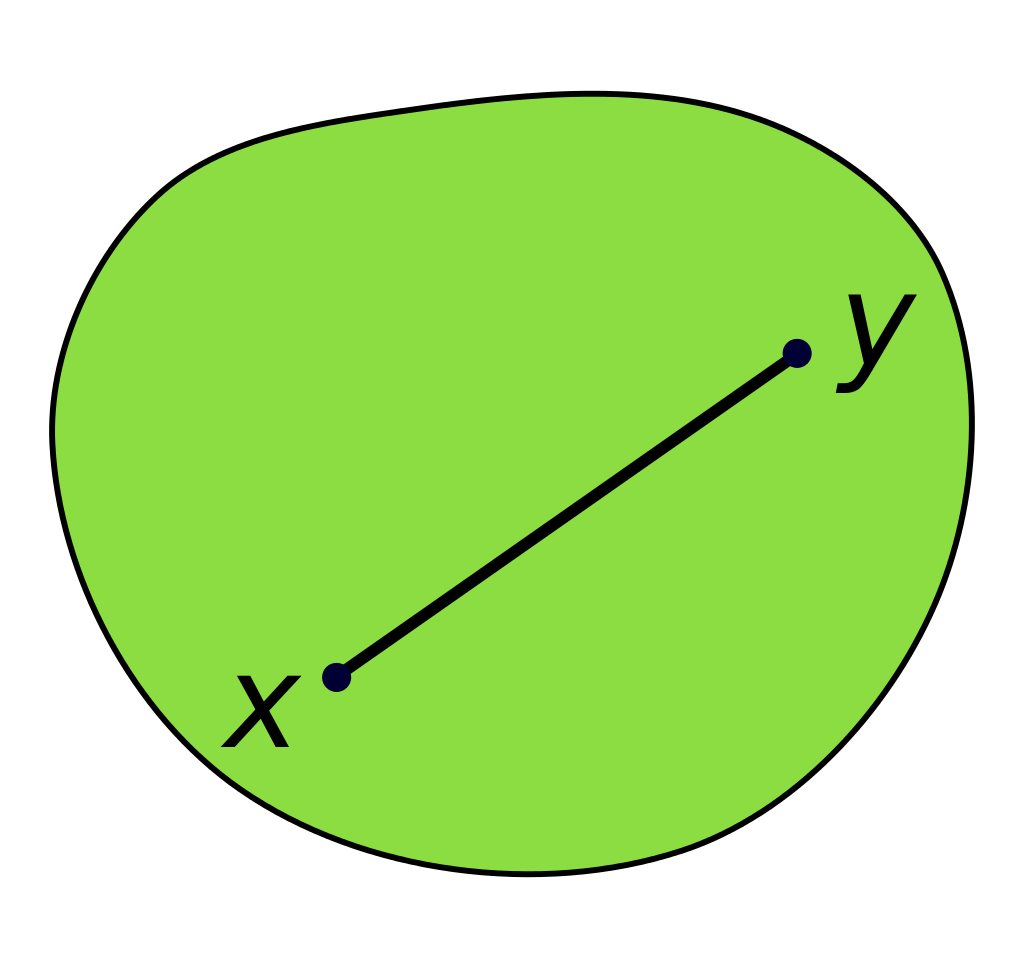
\includegraphics[width=0.8\textwidth]{figures/Convex_polygon_illustration1.png}
        \caption{Κυρτό Σύνολο}
        \label{fig:eg_convex_set}
    \end{subfigure}
    \hfill
    \begin{subfigure}[b]{.4\textwidth}
        \centering
        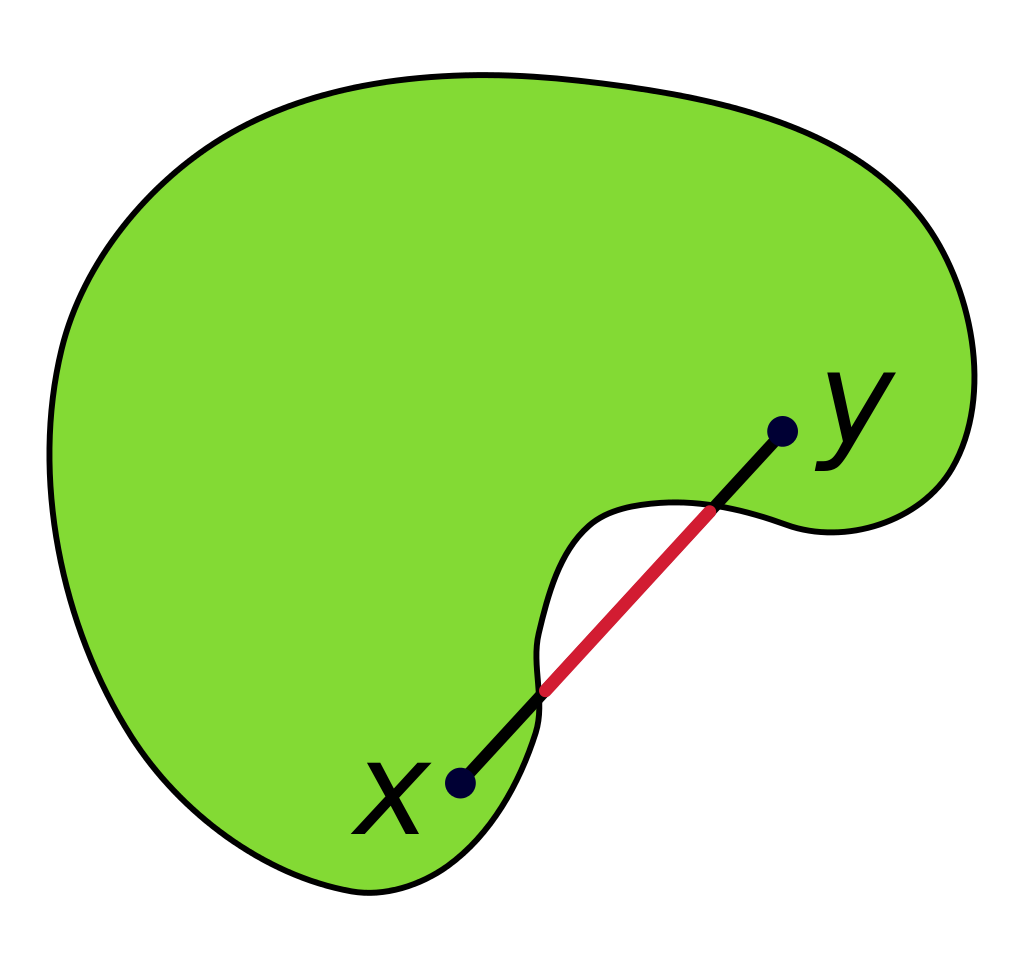
\includegraphics[width=0.8\textwidth]{figures/Convex_polygon_illustration2.png}
        \caption{Μη Κυρτό Σύνολο}
        \label{fig:eg_nonconvex_set}
    \end{subfigure}
    \caption{Κυρτά Σύνολα}
\end{figure}
\subsection{Κυρτό Σύνολο} Ένα σύνολο $C \subseteq \mathbf{R}^n$ ονομάζεται \textbf{κυρτό} αν το τμήμα
γραμμής μεταξύ δύο οποιοδήποτε σημείων που ανήκουν στο $C$, βρίσκεται στο
$C$. Για παράδειγμα αν για οποιοδήποτε $x_1, x_2 \in C$ και
$0 \leq \theta \leq 1$ τότε
\begin{equation*}
    x = \theta x_1 + (1 - \theta) x_2 \in C.
\end{equation*}

Ένα παράδειγμα κυρτού συνόλου παρουσιάζεται στο \ref{fig:eg_convex_set}, ενώ
αντιθέτως το σύνολο της \ref{fig:eg_nonconvex_set} δεν είναι κυρτό καθώς
μέρος του τμήματος της γραμμής μεταξύ των σημείων $x$ και $y$ δεν περιλαμβάνεται
στο σύνολο. Το σημείο της μορφής $\theta_1 x_1 + \dots + \theta_k
x_k$, όπου $\theta_1 + \dots + \theta_k = 1$ και $\theta_i \geq 0$ για $i = 1,
\dots ,k$, αναφέρεται ως \textbf{κυρτός
συνδυασμός} των σημείων $x_1 + \dots + x_k$. Το σύνολο όλων των κυρτών
συνδυασμών των σημείων του συνόλου $C \subseteq \mathbf{R}^n$
ονομάζεται \textbf{κυρτή θήκη} του $C$ και συμβολίζεται με
$\textbf{\tl{conv}} \ C$.

\subsection{Κυρτός κώνος} Το σύνολο $C$ ονομάζεται \textbf{κώνος}, αν για κάθε $x
\in C$ και $\theta \geq 0$ ισχύει ότι $\theta x \in C$. Το σύνολο $C$ είναι
\textbf{κυρτός κώνος} αν είναι κυρτό και κώνος, που σημαίνει ότι για οποιαδήποτε
$x_1, x_2 \in C$ και $\theta_1, \theta_2 \geq 0$ ισχύει
\begin{equation*}
    x = \theta_1 x_1 + \theta_2 x_2 \in C.
\end{equation*}
Στο σχήμα \ref{fig:convex_cone} παρουσιάζεται ένας κυρτός κώνος (ανοιχτό μπλε).
Μέσα σε αυτό, ο ροζ κυρτός κώνος αποτελείται από όλα τα σημεία
$\alpha x + \beta y$ με $\theta_1, \theta_2 \geq 0$.
\begin{figure}[h]
    \centering
    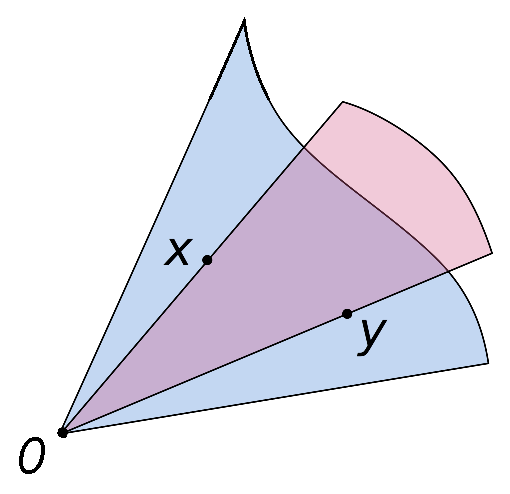
\includegraphics[scale=0.7]{figures/Convex_cone_illust.eps}
    \caption{Κυρτός Κώνος}
    \label{fig:convex_cone}
\end{figure}

\section{Σημαντικά Παραδείγματα}

\subsection{Υπερεπίπεδα} Ένα υπερεπίπεδο είναι ένα σύνολο της μορφής
\begin{equation*}
    \{ x \mid a^Tx = b \},
\end{equation*}
όπου $a \in \mathbf{R}^n, a \neq 0$ και $b \in \mathbf{R}^n$. Αναλυτικά είναι το
σύνολο λύσεων των γραμμικών εξισώσεων των συνιστωσών $x$. Γεωμετρικά το
υπερεπίπεδο μπορεί να ερμηνευτεί ως το σύνολο των σημείων με σταθερό εσωτερικό
γινόμενο ως προς το διάνυσμα $a$, ή ως το υπερεπίπεδο με κανονικό διάνυσμα
$a$, και η σταθερά $b$ καθορίζει την απόσταση του υπερεπιπέδου από την αρχή. Τα
υπερεπίπεδα είναι αφινικά και κυρτά.

\subsection{Ημιχώρος} Ένα υπερεπίπεδο χωρίζει το $\mathbf{R}^n$ σε δύο
\textbf{ημιχώρους}. Ένας (κλείστος) ημιχώρος είναι το σύνολο της μορφής
\begin{equation*}
    \{ x \mid a^Tx \leq b \},
\end{equation*}
όπου $a \neq 0$, π.χ., το σύνολο λύσης μίας ανισότητας. Οι ημιχώροι είναι κυρτοί
αλλά όχι αφινικοί.

\subsection{(Ευκλείδειες) Μπάλες} Μία \textbf{(Ευκλείδεια) μπάλα} στο $\mathbf{R}^n$
έχει τη μορφή
\begin{equation*}
    B(x_c, r) = \{x \mid \|x - x_c\|_2 \leq r\} = \{x \mid (x - x_c)^T(x - x_c) \leq
    r^2\},
\end{equation*}
όπου $r > 0$, και $\| \cdot \|_2$ συμβολίζει την Ευκλείδεια νόρμα. Το διάνυσμα
$x_c$ είναι το \emph{κέντρο} της μπάλας και το βαθμωτό μέγεθος $r$ η
\emph{ακτίνα} της.
Η μπάλα $B(x_c, r)$ αποτελείται από όλα τα σημεία που απέχουν το πολύ απόσταση
ίση με $r$ από το κέντρο $x_c$ και είναι κυρτό σύνολο.

\subsection{Ελλειψοειδές} Μία συγγενική κατηγορία κυρτού συνόλου είναι το
\textbf{ελλειψοειδές}, που περιγράφεται
\begin{equation*}
    \mathcal{E} = \{x \mid (x - x_c)^T P^{-1}(x - x_c) \leq 1\},
\end{equation*}
όπου $P = P^T > 0$, π.χ., το μητρώο $P$ είναι συμμετρικό και θετικά ορισμένο. Το
διάνυσμα $x_c \in \mathbf{R}^n$ είναι το \emph{κέντρο} του ελλειψοειδούς. Το
μητρώο $P$ καθορίζει κατά πόσο το ελλειψοειδές επεκτείνεται σε κάθε διεύθυνση
από το $x_c$. Το μήκος των ημιαξόνων του $\mathcal{E}$ δίνονται από τα
$\sqrt{\lambda_i}$, όπου $\lambda_i$ είναι οι ιδιοτιμές του $P$.

\subsection{Νόρμα} Μία συνάρτηση $\| \cdot \|$ που ικανοποιεί
\begin{itemize}
    \item $\|x\| \geq 0$ και $\|x\| = 0$ αν και μόνο αν $x = 0$,
    \item $\|tx\| = |t|\|x\|$ για κάθε $t \in \mathbf{R}$,
    \item $\|x + y\| \leq \|x\| + \|y\|$,
\end{itemize}
είναι \textbf{νόρμα}. Ο συμβολισμός $\| \cdot \|$ αποτελεί γενικό συμβολισμό,
συνήθως χρησιμοποιούμε κάποιο συμβολισμό για να προσδιορίσουμε τον τύπο της
νόρμας.

\subsection{Νορμική μπάλα και νορμικός κώνος} Θεωρώντας οποιαδήποτε νόρμα
$\| \cdot \|$ στο $\mathbf{R}^n$ και από τις ιδιότητες της νόρμας, η
\textbf{νορμική μπάλα} ακτίνας $r$ και κέντρου $x_c$ που περιγράφεται από
$\{ x \mid \|x - x_c\| \leq r\}$, είναι κυρτή. Ο \textbf{νορμκός κώνος}
εφοδιασμένος με τη νόρμα $\| \cdot \|$ είναι το σύνολο
\begin{equation*}
    C = \{(x,t) \mid \|x\| \leq t\} \subseteq \mathbf{R}^{n+1},
\end{equation*}
και είναι κυρτός κώνος.

\subsection{Πολύεδρα} Το \textbf{πολύεδρο} ορίζεται ως το σύνολο λύσης πεπερασμένων
γραμμικών ισοτήτων και ανισοτήτων:
\begin{equation*}
    \mathcal{P} = \{x \mid a_j^T x \leq b_j,\ j = 1, \dots, m,\ c_j^T x = d_j,\
    j = 1, \dots, p \}.
\end{equation*}
Το πολύεδρο είναι ουσιαστικά η τομή πεπερασμένων ημιχώρων και υπερεπιπέδων.
Αφινικά σύνολα (π.χ. υποχώροι, υπερεπίπεδα, γραμμές), τμήματα γραμμής και
ημιχώροι είναι όλα πολύεδρα. Επίσης, εύκολα αποδεικνύεται ότι τα πολύεδρα είναι
κυρτά σύνολα. Ένα φραγμένο πολύεδρο πολλές φορές καλείται \textbf{πολύτοπο}.
Πολλές φορές είναι βολική η συμπαγής μορφή του πολυέδρου
\begin{equation*}
    \mathcal{P} = \{x \mid Ax \leq = b, Cx = d\}.
\end{equation*}

\textbf{\tl{Simplexes}}. Τα \textbf{\tl{simplexes}} είναι μία
σημαντική κατηγορία πολυέδρων. Έστω τα $k + 1$ σημεία $v_0, \dots, v_k \in
\mathbf{R}^n$ είναι \textbf{αφινικά ανεξάρτητα}, που σημαίνει ότι $v_1 - v_0, \dots,
v_k - v_0$ είναι γραμμικώς ανεξάρτητα. Το \tl{simplex} τότε καθορίζεται από τη σχέση
\begin{equation*}
    \mathcal{C} = \textbf{\tl{conv}}\ \{v_0, \dots, v_k\} =
    \{ \theta_0 v_0 + \dots + \theta_k v_k \mid \theta \geq 0,\ \vc{1}^T\theta
    = 1\},
\end{equation*}
όπου το $\vc{1}$ συμβολίζει το διάνυσμα με όλα τα στοιχεία μονάδα. Η αφινική
διάσταση αυτού του συμπλέγματος είναι $k$, έτσι πολλές φορές λέγεται
$k$-διάστασης \tl{simplex} στο $\mathbf{R}^n$.

\textbf{Κυρτή θήκη και πολύεδρα}. Η κυρτή θήκη του πεπερασμένου συνόλου
$\{v_1,\dots,v_k\}$ είναι
\begin{equation*}
    \textbf{\tl{conv}}\ \{v_1,\dots,v_k\} = \{\theta_1 v_1+\dots+\theta_k v_k
    \mid \theta \geq 0,\ \vc{1}^T\theta = 1\}.
\end{equation*}
Το σύνολο αυτό είναι πολύεδρο και φραγμένο.

\subsection{Θετικά ημιορισμένος κώνος} Με το συμβολισμό $\mathbf{S}^n$ δηλώνουμε
το σύνολο των συμμετρικών $n \times n$ μητρώων,
\begin{equation*}
    \mt{S}^n = \{ X \in \mt{R}^{n \times n} \mid X = X^T\},
\end{equation*}
που είναι διανυσματικός χώρος διάστασης $n(n+1)/2$. Με το συμβολισμό
$\mathbf{S}_+^n$ δηλώνουμε το σύνολο των συμμετρικών θετικά ημιορισμένων μητρώων
\begin{equation*}
    \mt{S}_+^n = \{ X \in \mt{S}^{n} \mid X \geq 0\},
\end{equation*}
που είναι κυρτός κώνος και με το συμβολισμό $\mathbf{S}_{++}^n$ δηλώνουμε
το σύνολο των συμμετρικών θετικά ορισμένων μητρώων
\begin{equation*}
    \mt{S}_{++}^n = \{ X \in \mt{S}^{n} \mid X > 0\}.
\end{equation*}

\section{Πράξεις που διατηρούν την κυρτότητα}

\subsection{Τομή} Η κυρτότητα διατηρείται υπό την τομή συνόλων, αν $S_1$
και $S_2$ είναι κυρτά σύνολα, τότε η τομή $S_1 \cap S_2$ είναι κυρτή.
Η ιδιότητα αυτή επεκτείνεται για τομή απείρων συνόλων. Ένα απλό παράδειγμα
είναι το πολύεδρο που είναι η τομή ημιχώρων και υπερεπιπέδων, που είναι κυρτά,
και επομένως είναι κυρτό.

\subsection{Αφινικές συναρτήσεις} Μία συνάρτηση $f:\mathbf{R}^n \to \mathbf{R}^m$
είναι \textbf{αφινική} αν είναι το άθροισμα γραμμικών συναρτήσεων και σταθεράς.
Για παράδειγμα συνάρτηση της μορφής $f(x) = \mt{A}x + b$, όπου $\mt{A} \in
\mathbf{R}^{n\times m}$ και $b \in \mathbf{R}^m$. Έστω $S \subseteq
\mathbf{R}^n$ είναι κυρτό και $f:\mathbf{R}^n \to \mathbf{R}^m$ είναι αφινική
συνάρτηση. Τότε η εικόνα του $S$ υπό τον περιορισμό της $f$,
\begin{equation*}
    f(S) = \{ f(x) \mid x \in S\},
\end{equation*}
είναι κυρτή.Αντίστοιχα, αν $f:\mathbf{R}^k \to \mathbf{R}^n$ είναι αφινική
συνάρτηση, η αντίστροφη εικόνα του $S$ υπό τον περιορισμό της $f$,
\begin{equation*}
    f^{-1}(S) = \{ x \mid f(x) \in S\},
\end{equation*}
είναι κυρτή.Κάποια απλά παραδείγματα αφινικών συναρτήσεων είναι η
\textbf{κλιμάκωση} και η \textbf{μετατόπιση}. Αν $S \subseteq \mathbf{R}^n$
είναι κυρτό, $\alpha \in \mathbf{R}$ και $a \in \mathbf{R}^n$, τότε τα σύνολα
$\alpha S$ και $S + a$ είναι κυρτά, όπου
\begin{equation*}
    \alpha S = \{\alpha x \mid x\in S\}, \qquad S + a = \{x + a \mid x\in S\}.
\end{equation*}
Επίσης, το σύνολο λύσης \textbf{γραμμικών μητρώων ανισότητας}
(\tl{linear matrix inequality, LMI}), $\{x\mid A(x) \leq B\}$ είναι
κυρτό, όπου $B, A_i \in \mathbf{S}^m$.

\subsection{Γραμμική-κλασματική και προοπτική συνάρτηση}

\textbf{Συνάρτηση προοπτικής}. Ορίζουμε τη συνάρτηση προοπτικής $P :\
\mathbf{R}^n \to \mathbf{R}^n$, με πεδίο ορισμού $\textbf{\tl{dom}} \ P =
\mathbf{R}^n \times \mathbf{R}_{++}$, ως, όπου $\mathbf{R}_{++}$ δηλώνει το
σύνολο των πραγματικών θετικών αριθμών, $P(z, t) = z/t$. Η συνάρτηση αυτή
κλιμακώνει ή κανονικοποιεί διανύσματα ώστε η τελευταία συνιστώσα να γίνει μονάδα
και στη συνέχεια την αποβάλει. Το σημαντικό είναι ότι αν $C \subseteq
\textbf{\tl{dom}}\ P$ είναι κυρτό, τότε και η εικόνα
\begin{equation*}
    P(C) = \{P(x) \mid x \in C\},
\end{equation*}
υπό τη συνάρτηση προοπτικής είναι κυρτή. Επίσης, η αντίστροφη εικόνα ενός κυρτού
συνόλου υπό συνάρτηση προοπτικής είναι κυρτή, δηλαδή αν $C \subseteq
\mathbf{R}^n$ είναι κυρτό, τότε
\begin{equation*}
    P^{-1}(C) = \{(x, t) \in \mathbf{R}^{n + 1} \mid x/t \in C,\ t > 0\},
\end{equation*}
είναι κυρτή.

\textbf{Γραμμική-κλασματική συνάρτηση}. Μία \textbf{γραμμική-κλασματική
συνάρτηση} σχηματίζεται από τη σύνθεση συναρτήσεων προοπτικής με αφινικές
συναρτήσεις. Έστω $g: \ \mathbf{R}^n \to \mathbf{R}^{m+1}$ αφινική, π.χ.,
\begin{equation*}
    g(x) = \begin{pmatrix} A \\ c^T \end{pmatrix}x + \begin{pmatrix} b \\ d
    \end{pmatrix},
\end{equation*}
όπου $A \in \mathbf{R}^{m \times n}, b \in \mathbf{R}^m, c \in \mathbf{R}^n$,
και $d \in \mathbf{R}$. Η συνάρτηση $f: \ \mathbf{R}^n \to \mathbf{R}^{m}$,
δίνεται από $f = P \circ g$, η σύμφωνα με το παραπάνω παράδειγμα
\begin{equation*}
    f(x) = (Ax + b) / (c^Tx + d), \qquad \textbf{\tl{dom}}\ f = \{x \mid c^Tx + d >
    0\},
\end{equation*}
καλείται \textbf{γραμμική-κλασματική} (ή \textbf{προβολική}) συνάρτηση. Αν $c =
0$ και $d>0$, το πεδίο ορισμού της $f$ είναι το $\mathbf{R}^n$ και η $f$ είναι
αφινική συνάρτηση. Έτσι μπορούμε να θεωρήσουμε της αφινκές και τις γραμμικές
συναρτήσεις σαν ειδικές περιπτώσεις γραμμικών-κλασματικών συναρτήσεων. Όπως και
στην προηγούμενη περίπτωση, η εικόνα και η αντίστροφη εικόνα κυρτών συνόλων υπό
γραμμικών-κλασματικών συναρτήσεων είναι κυρτά σύνολα.

\section{Γενικευμένες ανισότητες}

\subsection{Γνήσιοι κώνοι και γενικευμένες ανισότητες} Ένας κώνος $K \subseteq
\mathbf{R}^n$ καλείται \textbf{γνήσιος κώνος} αν ικανοποιεί τα παρακάτω:
\begin{itemize}
    \item $K$ είναι κυρτό.
    \item $K$ είναι κλειστό.
    \item $K$ είναι στερεό, που σημαίνει ότι έχει μη-κενά εσωτερικά σημεία.
    \item $K$ είναι σημειακό (\tl{pointed}), που σημαίνει ότι δεν περιέχει καμία
        ευθεία (ή ισοδύναμα, $x \in K, -x \in K \Rightarrow x = 0$).
\end{itemize}
Ένας γνήσιος κώνος $K$ μπορεί να χρησιμοποιηθεί για να ορίσουμε τη
\textbf{γενικευμένη ανισότητα}, που είναι μερικώς διατεταγμένο στο
$\mathbf{R}^n$ και έχει πολλές ιδιότητες της τυπικής διατεταγμένης του
$\mathbf{R}$. Συνδέουμε με το γνήσιο κώνο $K$ το μερικώς διατεταγμένο σύνολο στο
$\mathbf{R}^n$ που ορίζεται από
\begin{equation*}
    x \leq {}_Ky \Leftrightarrow y - x \in K.
\end{equation*}
Επίσης, γράφουμε $x \geq_Ky$ για $y \leq_K x$. Αντίστοιχα, ορίζουμε την
\textbf{αυστηρή γενικευμένη ανισότητα} και συνδέουμε το γνήσιο κώνο με το
αυστηρό μερικώς διατεταγμένο σύνολο ως
\begin{equation*}
    x \leq_Ky \Leftrightarrow y - x \in \textbf{\tl{int}}\ K,
\end{equation*}
και γράφουμε $x >_K y$ για $y <_K x$. Κάποια τυπικά παραδείγματα είναι π.χ.
όταν $K = \mathbf{R}_+^n$, τότε η γενικευμένη ανισότητα $\leq_K$ αντιστοιχεί
σε ανισότητα ως προς την κάθε συνιστώσα μεταξύ διανυσμάτων: $x \leq_K y$
σημαίνει ότι $x_i \leq y_i$, για $i = 1, \dots, n$. Ακόμη, ο θετικά
ημιορισμένος κώνος $\mathbf{S}^n_+$ είναι ένας γνήσιος κώνος στο $\mathbf{S}^n$.
Η αντίστοιχη γενικευμένη ανισότητα $\leq_K$ είναι η ανισότητα μητρώων
$X \leq_K Y$ που σημαίνει ότι $Y - X$ είναι θετικά ημιορισμένο. Επίσης, οι
γενικευμένες ανισότητες $\leq_K$ έχουν όμοιες ιδιότητες με τη γνωστή ανισότητα
$\leq$ του $\mathbf{R}$.

\subsection{Ελάχιστο και ελαχιστοτικό στοιχείο} Ενώ πολλές από τις ιδιότητες των
γενικευμένων ανισοτήτων βρίσκονται σε αναλογία με αυτές του $\mathbf{R}$, αυτό
δεν συμβαίνει για όλες. Η πιο εμφανής διαφορά είναι ότι η $\leq$ στο
$\mathbf{R}$ είναι γραμμικώς διατεταγμένη, δηλαδή κάθε δύο σημεία είναι
συγκρίσιμα. Η ιδιότητα αυτή δεν ισχύει για τις γενικευμένες ανισότητες και αυτό
ως συνέπεια οι έννοιες του ελάχιστου και μέγιστου να χρήζουν ορισμού. Λέμε ότι
$x \in S$ είναι το \textbf{ελάχιστο} στοιχείο του $S$, σε σχέση με τη γενικευμένη
ανισότητα $\leq_K$, αν για κάθε $y \in S$ ισχύει $x \leq_K y$. Ορίζουμε το
\textbf{μέγιστο} στοιχείο του $S$, σε σχέση με τη γενικευμένη ανισότητα με τον
αντίστοιχο προφανή τρόπο. Αν ένα σύνολο έχει ελάχιστο (μέγιστο) στοιχείο, τότε
είναι μοναδικό. Μία παρόμοια έννοια είναι το \textbf{ελαχιστοτικό στοιχείο}
(\textbf{\tl{minimal element}}). Λέμε ότι $x \in S$ είναι το ελαχιστοτικό
στοιχείο του $S$, σε σχέση με τη γενικευμένη ανισότητα $\leq_K$,
αν $y \in S$ ισχύει $y \leq_K x$ μόνο όταν $y = x$. Αντίστοιχα για το
\textbf{μεγιστοτικό στοιχείο} (\textbf{\tl{maximal element}}).

\section{Υπερεπίπεδο διαχωριστικό και στήριξης}

\subsection{Θεώρημα διαχωριστικού υπερεπιπέδου} Έστω $C$ και $D$ μη-κενά ξένα κυρτά
σύνολα, δηλαδή $C \cap D = \emptyset$. Τότε υπάρχει $a \neq 0$ και $b$ τέτοια
ώστε $a^Tx \leq b$ για όλα τα $x \in C$ και $a^tx \geq b$ για όλα τα $x \in D$.
Με άλλα λόγια, η αφινική συνάρτηση $a^T x - b$ είναι μη-θετική στο $C$ και
μη-αρνητική στο $D$. Το υπερεπίπεδο $\{x \mid a^T x = b\}$ ονομάζεται
\textbf{διαχωριστικό υπερεπίπεδο} για τα σύνολα $C$ και $D$, ή λέμε ότι
\textbf{διαχωρίζει} το σύνολο $C$ και $D$. Σχηματικά το θεώρημα παρουσιάζεται
στο γράφημα \ref{fig:seperating_theorem}.
\begin{figure}[h]
    \centering
    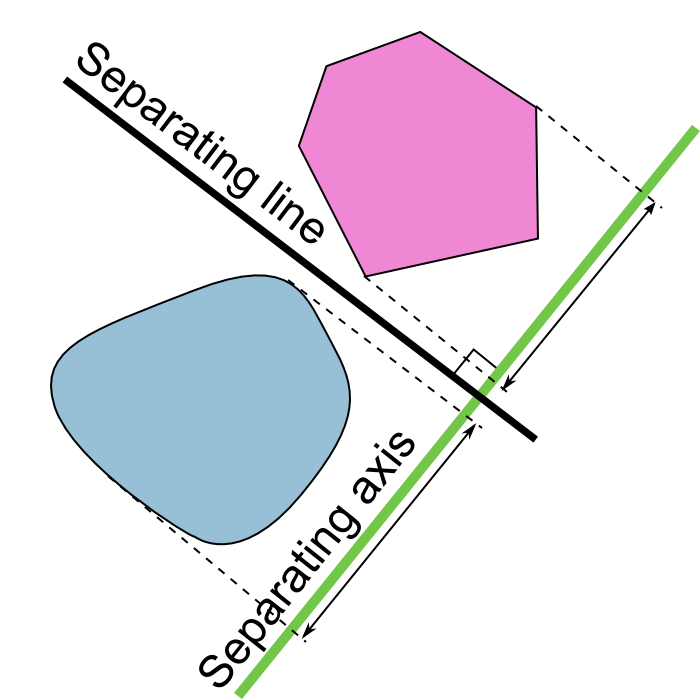
\includegraphics[scale=0.3]{figures/Separating_axis_theorem2008.png}
    \caption{Θεώρημα διαχωριστικού υπερεπιπέδου}
    \label{fig:seperating_theorem}
\end{figure}
Όπως ορίστηκε το παραπάνω θεώρημα, αν ισχύει μόνο η ανισότητα, και στις δύο
σχέσεις, τότε έχουμε το \textbf{αυστηρό διαχωριστικό υπερεπίπεδο}.

\subsection{Θεώρημα υπερεπιπέδου στήριξης} Έστω $C \subseteq \mathbf{R}^n$,
και $x_0$ είναι σημείο του συνόρου
\begin{equation*}
    x_0 \in \textbf{\tl{bd}}\ C.
\end{equation*}
Αν $a \neq 0$ ικανοποιεί $a^Tx \leq a^Tx_0$ για όλα τα $x \in C$, τότε το
υπερεπίπεδο $\{x \mid a^Tx = a^Tx_0\}$ ονομάζεται \textbf{υπερεπίπεδο στήριξης}
του $C$ στο $x_0$. Ισοδύναμα μπορούμε πούμε ότι το σημείο $x_0$ και το σύνολο
$C$ διαχωρίζονται από το υπερεπίπεδο $\{x\mid a^Tx = a^T x_0\}$. Γεωμετρικά,
όπως φαίνεται στο \ref{fig:supporting_theorem}, το υπερεπίπεδο είναι η εφαπτομένη του $C$ στο $x_0$ και ο
υποχώρος $\{x \mid a^Tx \leq a^Tx_0\}$ περιέχει το $C$.
\begin{figure}[h]
    \centering
    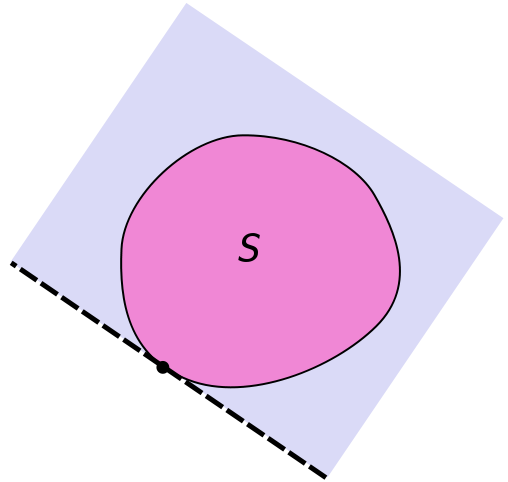
\includegraphics[scale=0.3]{figures/Supporting_hyperplane1.png}
    \caption{Θεώρημα υπερεπιπέδου στήριξης}
    \label{fig:supporting_theorem}
\end{figure}
Ένα βασικό αποτέλεσμα, που ονομάζεται \textbf{θεώρημα υπερεπιπέδου στήριξης},
δηλώνει ότι για κάθε μη-κενό κυρτό σύνολο $C$, και για οποιοδήποτε $x_0 \in
\textbf{\tl{bd}}\ C$, τότε υπάρχει υπερεπίπεδο στήριξης του $C$ στο $x_0$.

\section{Δυϊκός κώνος και γενικευμένες ανισότητες}

\subsection{Δυϊκός κώνος} Έστω $K$ κώνος. Το σύνολο
\begin{equation*}
    K^* = \{y \mid x^T y \geq 0 \ \text{για όλα τα} \ x \in K\}
\end{equation*}
ονομάζεται \textbf{δυϊκός κώνος} του $K$. Όπως υποδηλώνει το όνομα, $K^*$ είναι
κώνος και είναι πάντα κυρτός, ακόμα και αν ο κώνος $K$ δεν είναι. Για
παραδείγματα ο κώνος $\mathbf{R}^n_+$ είναι ο ίδιος δυΐκος
\begin{equation*}
    x^Ty \geq 0 \ \text{για όλα τα} \ x \geq 0 \Leftrightarrow y \geq 0
\end{equation*}
και λέμε τους κώνους αυτούς \textbf{αυτοδυϊκούς}.

\subsection{Δυϊκές γενικευμένες ανισότητες} Αν ο κυρτός κώνος $K$ είναι γνήσιος,
άρα επάγεται μία γενικευμένη ανισότητα $\leq_K$. Τότε ο δυϊκός κώνος είναι
επίσης γνήσιος, και επάγει μία γενικευμένη ανισότητα. Αναφερόμαστε στη
γενικευμένη ανισότητα $\leq_{K^*}$ ως τη \textbf{δυϊκή} της γενικευμένης
ανισότητας $\leq_{K}$. Μερικές σημαντικές ιδιότητες σχετικά με τη γενικευμένη
ανισότητα και την δυϊκή της είναι
\begin{itemize}
    \item $x \leq_K y$ αν και μόνο αν $\lambda^T x \leq \lambda^T y$ για κάθε
        $\lambda \geq_{K^*} 0$.
    \item $x <_K y$ αν και μόνο αν $\lambda^T x < \lambda^T y$ για κάθε
        $\lambda \geq_{K^*} 0$, $\lambda \neq 0$.
\end{itemize}

\subsection{Ελάχιστα και ελαχιστοτικά στοιχεία μέσω δυϊκών ανισοτήτων}

Χρησιμοποιώντας τις δυϊκές γενικευμένες ανισότητες μπορούμε να χαρακτηρίσουμε
ελάχιστα και ελαχιστοτικά στοιχεία (κυρτών ή όχι) συνόλων $S \subseteq
\mathbf{R}^m$ ως προς τις γενικευμένες ανισότητες που επάγονται από το γνήσιο
κώνο $K$.

\textbf{Δυϊκός χαρακτηρισμός ελάχιστου στοιχείου}. Το $x$ είναι
\textbf{ελάχιστο} στοιχείο του $S$, ως προς τη γενικευμένη ανισότητα $\leq_K$,
αν και μόνο αν για κάθε $\lambda >_{K^*} 0$, το $x$ είναι το μοναδικό που
ελαχιστοποιεί τη σχέση $\lambda^T z$ για $z \in S$. Γεωμετρικά, αυτό σημαίνει ότι για
κάθε $\lambda >_{K^*} 0$, το υπερεπίπεδο
\begin{equation*}
    \{z \mid \lambda^T(z - x) = 0\}
\end{equation*}
είναι ένα αυστηρό υπερεπίπεδο στήριξης του $S$ στο $x$. Αυστηρό
υπερεπίπεδο στήριξης σημαίνει ότι το υπερεπίπεδο τέμνει το $S$ μόνο
στο $x$. Η κυρτότητα του συνόλου $S$ δεν είναι απαραίτητη σύμφωνα με το
παραπάνω.

\textbf{Δυϊκός χαρακτηρισμός ελαχιστοτικού στοιχείου}. Αν το $x$ ελαχιστοποιεί
$\lambda^Tz$ για $z\in S$ και $\lambda >_{K^*} 0$ τότε το $x$ είναι
\textbf{ελαχιστοτικό}. Το αντίστροφο δεν ισχύει στη γενική περίπτωση, ένα σημείο
$x$ μπορεί να είναι ελαχιστοτικό του $S$, αλλά να μην ελαχιστοποιεί τη σχέση
$\lambda^Tz$ για $z\in S$ και οποιοδήποτε $\lambda$. Αν το σύνολο $S$
είναι κυρτό τότε για κάθε ελαχιστοτικό στοιχείο $x$ υπάρχει μη μηδενικό
$\lambda \leq_{K^*} 0$ τέτοιο ώστε το $x$ να ελαχιστοποιεί τη $\lambda^Tz$ για
$z\in S$.

\clearemptypage

\chapter{Μέθοδοι Εσωτερικού Σημείου}\label{ch:ip}
\section{Ιστορικά στοιχεία}
Ο γραμμικός προγραμματισμός σύμφωνα με το βιβλίο \cite{wright1997primal}
είναι ένας από τους πιο πετυχημένους τομείς της
βελτιστοποίησης. Από τη διατύπωσή του τη δεκαετία του \(1930\) μέχρι την
ανάπτυξη του αλγορίθμου \tl{simplex} τη δεκαετία του \(1940\) από τον
\tl{Dantzig}, γενιές εργαζομένων στα οικονομικά, στη μηχανική και άλλους τομείς
εκπαιδεύτηκαν για να λύνουν προβλήματα γραμμικού προγραμματισμού. Ακόμα και όταν
τα μοντέλα ήταν μη-γραμμικά, γραμμικές μέθοδοι χρησιμοποιούνταν λόγω της μεγάλης
ανάπτυξης που είχαν.

Η δημοσίευση το \(1948\) του \tl{Karmarkar} \cite{karmarkar1984} ήταν το πιο σημαντικό γεγονός στο
γραμμικό προγραμματισμό μετά την ανακάλυψη της μεθόδου \tl{simplex}. Ο λόγος
ήταν ότι ο αλγόριθμος του \tl{Karmarkar} υποσχόταν πολυωνυμική πολυπλοκότητα, σε
σύγκριση με τη λογαριθμική πολυπλοκότητα της μεθόδου \tl{simplex}, και
εξαιρετική πρακτική επίδοση σε μεγάλου μεγέθους προβλήματα. Οι ισχυρισμοί αυτοί
δεν επιβεβαιώθηκαν, αλλά η δημοσίευση έδωσε μία επανάσταση στην έρευνα του
γραμμικού προγραμματισμού που οδήγησε σε έναν νέο τομέα αλγορίθμων που
ονομάζονται μέθοδοι εσωτερικού σημείου. Στις παρακάτω ενότητες θα περιγράψουμε
κάποιους τυπικούς αλγορίθμους εσωτερικών σημείων. Θα ξεκινήσουμε με τη μέθοδο
\tl{affine scaling} που αποτελεί μία εισαγωγή για τον αλγόριθμο του
\tl{Karmarkar}, τη βάση τις οικογένειας αλγορίθμων εσωτερικού σημείου. Στη
συνέχεια θα παρουσιάσουμε τους αλγορίθμους \tl{path-following} (ή μέθοδος
φράγματος) και \tl{primal-dual} που κυρίως χρησιμοποιούνται σε πρακτικές
εφαρμογές στις μέρες μας.

\section{Μέθοδος \tl{affine scaling}}
Σε αυτή την ενότητα θα περιγράψουμε έναν απλό αλγόριθμο, που ονομάζεται
\tl{affine scaling}, για την επίλυση προβλημάτων γραμμικών προγραμματισμού,
βασιζόμενοι στο βιβλίο \cite{chong2010}. Η μέθοδος αυτή είναι μία μέθοδος
εσωτερικού σημείου και επιτελεί το ρόλο εισαγωγής στον αλγόριθμο του
\tl{Karmarkar}. Γενικά, οι μέθοδοι εσωτερικού σημείου διαφέρουν από τη μέθοδο
\tl{simplex} σε ένα βασικό σημείο: η μέθοδος εσωτερικού σημείου ξεκινάει στο
εσωτερικού του εφικτού συνόλου και κινείται σε αυτό για την εύρεση βέλτιστου
σημείου. Αντίθετα, η μέθοδος \tl{simplex} κινείται στις κορυφές του εφικτού
συνόλου.

Έστω το γραμμικό πρόβλημα
\begin{equation*}
    \begin{aligned}
        & {\text{\tl{minimize}}}
        & & c^T x \\
        & \text{\tl{subject to}}
        & & A x = b \\
        &&& x \ge 0.
    \end{aligned}
\end{equation*}
Έστω ότι έχουμε το εφικτό σημείο \( x^{(0)} \) που είναι αυστηρώς εσωτερικό
(δηλαδή \( x > 0\)). Θέλουμε να βρούμε ένα νέο σημείο \( x^{(1)} \) ψάχνοντας
στη διεύθυνση του \( d^{(0)} \) που μειώνει την αντικειμενική συνάρτηση. Δηλαδή
\begin{equation*}
    x^{(1)} = x^{(0)} + a_0 d^{(0)},
\end{equation*}
με \(a_0\) το μέγεθος του βήματος. Προκειμένου το \( x^{(1)} \) να βρίσκεται
εντός του εφικτού συνόλου, είναι απαραίτητο το διάνυσμα \( d^{(0)} \) να
βρίσκεται στο μηδενοχώρο του \(A\), με άλλα λόγια θέλουμε να ισχύει
\( Ax^{(1)} = b\). Επειδή, το \( x^{(0)} \) είναι εφικτό σημείο από τις παραπάνω
εξισώσεις προκύπτει
\begin{equation*}
    A\left( x^{(1)} - x^{(0)} \right) = a_0Ad^{(0)} = 0.
\end{equation*}
Για να επιλέξουμε \( d^{(0)} \) που να βρίσκεται στο μηδενοχώρο του \(A \) και
να κινείται στην μείωση της αντικειμενικής, δηλαδή κοντά στο \(-c\), παίρνουμε την
ορθογώνια προβολή του \(-c\) στο μηδενοχώρο του \(A\). Αυτή η προβολή
περιγράφεται από τον πίνακα
\begin{equation*}
    P = I_n - A^T(AA^T){-1}A.
\end{equation*}
Έτσι θέτουμε το \( d^{(0)} \) να είναι στη διεύθυνση της ορθογώνιας προβολής του
\( -c \) στο μηδενοχώρο του \(A\)
\begin{equation*}
    d^{(0)} = - Pc,
\end{equation*}
και έτσι, βρίσκουμε ένα καινούργιο εφικτό σημείο \( x^{(1)} \) από τη σχέση
\begin{equation*}
    x^{(1)} = x^{(0)} - a_0Pc.
\end{equation*}

Παρατηρώντας τις σχέσεις καταλήγουμε στο συμπέρασμα ότι αν το αρχικό εφικτό
σημείο βρίσκεται στο \tl{``}κέντρο\tl{''} του εφικτού συνόλου, τότε μπορούμε να
κινηθούμε με μεγαλύτερο βήμα και αυτό σημαίνει μεγαλύτερη μείωση στην τιμή της
αντικειμενικής και άρα ταχύτερη σύγκλιση.

Στην περίπτωση που το αρχικό σημείο δεν βρίσκεται στο κέντρο του συνόλου,
μπορούμε με έναν αφηνικό μετασχηματισμό να το μετατρέψουμε σε κεντρικό. Για να
μετατρέψουμε το \( x^{(0)} \) στο κεντρικό σημείο \(e\), χρησιμοποιούμε τον
αφηνικό μετασχηματισμό (\tl{affine scaling transformation})
\begin{equation*}
    e = D_0^{-1}x^{(0)},
\end{equation*}
όπου \( D_0 = \text{\tl{diag}}\left[ x_1^{(0)}, \dots, x_n^{(n)} \right]\). Με την
υπόθεση που κάναμε ότι το \( x^{(0)} \) είναι αυστηρώς εσωτερικό, ο πίνακας
\(D_0 \) είναι αντιστρέψιμος. Προφανώς, στην πράξη δεν επιδιώκουμε να βρούμε το
κεντρικό σημείο αλλά κάποιο σημείο αρκετά κοντά σε αυτό με μικρή σχετικά
απόκλιση. Βασικό βέβαια είναι το αρχικό σημείο να είναι αυστηρώς εσωτερικό.

Με την παραπάνω διαδικασία, μετατρέψαμε το αρχικό εφικτό διάνυσμα
\( x^{(0)} \) με το μετασχηματισμό \( D_0^{-1} \) και ουσιαστικό αλλάξαμε βάση.
Έτσι στη νέα βάση το πρόβλημα της ενότητας μετασχηματίζεται στο
αντίστοιχο γραμμικό
\begin{equation*}
    \begin{aligned}
        & {\text{\tl{minimize}}}
        & & \bar{c}_0^T \bar{x} \\
        & \text{\tl{subject to}}
        & & \bar{A}_0 \bar{x} = b \\
        &&& \bar{x} \ge 0,
    \end{aligned}
\end{equation*}
όπου
\begin{equation*}
    \bar{c}_0 = D_0c, \quad \bar{A}_0 = AD_0.
\end{equation*}
Εφαρμόζοντας τη διαδικασία που περιγράψαμε παραπάνω στο νέο σύστημα
συντεταγμένων, υπολογίζουμε την επόμενη τιμή από τη σχέση
\begin{equation*}
    \bar{x}^{(1)} = \bar{x}^{(0)} - a_0\bar{P}_0\bar{c}_0,
\end{equation*}
με \( \bar{x}^{(0)} = D_0^{-1}x^{(0)} \). Το νέο σημείο στις αρχικές
συντεταγμένες δίνεται με το μετασχηματισμό \( x^{(1)} = D_0 \bar{x}^{(1)} \).
Επαναλαμβάνοντας τη διαδικασία για μία ακολουθία σημείων \( \{ x^{(k)} \} \), όπου
\begin{equation*}
    x^{(k+1)} = x^{(k)} + a_kd^{(k)},
\end{equation*}
με
\begin{align*}
    D_k &= \text{\tl{diag}}\left[ x^{(k)}_1, \dots, x_n^{(k)} \right] \\
    \bar{A}_k &= AD_k \\
    \bar{P}_k &= I_n - \bar{A}^T_k \left(\bar{A}_k\bar{A}_k^T
    \right)^{-1}\bar{A}_k \\
    d^{(k)} &= -D_k\bar{P}_kD_kc.
\end{align*}
Σε κάθε βήμα του αλγορίθμου πρέπει να εξασφαλίζουμε ότι το \( x^{(k)} \) είναι
αυστηρώς εσωτερικό. Η συνθήκη των περιορισμών ικανοποιείται λόγω του τρόπου που
επιλέξαμε το \( d^{(k)} \). Όμως, πρέπει ακόμα να εξασφαλίσουμε ότι
\(x_i^{(k)} > 0 \) για \( i = 1, \dots, n \), και αυτό γίνεται με την κατάλληλη
επιλογή του βήματος, \(a_k\).

Αναφέραμε ήδη ότι επιδιώκουμε μεγάλο βήμα, για αυτό το λόγο πραγματοποιούμε τον
αφινικό μετασχηματισμό στο αρχικό σημείο για να το μετατρέψουμε σε κεντρικό.
Όμως πρέπει να επιλέξουμε τέτοιο βήμα ούτως ώστε το νέο σημείο να είναι θετικό.
Για να το επιτύχουμε αυτό, ορίζουμε
\begin{equation*}
    r_k = \underset{\{i: d_i^{(k)} < 0\}} {\text{\tl{min}}}
    -\frac{x^{(k)}_i}{d^{(k)}_i},
\end{equation*}
που αντιπροσωπεύει το μεγαλύτερο βήμα \( a_k \) έτσι ώστε οι συνιστώσες του
\( x^{(k+1)} \) να είναι μη-αρνητικές και υπολογίζουμε το βήμα από τη σχέση
\( a_k = \alpha r_k \) με \( \alpha \in (0, 1) \). Τυπικές τιμές του συντελεστή
\( \alpha \) είναι \(0.9\) ή \(0.99\).

Σε αντίθεση με άλλες μεθόδους, η μέθοδος \tl{affine scaling} μέθοδος δε θα
φτάσει σε βέλτιστη λύση σε πεπερασμένο αριθμό βημάτων στη γενική περίπτωση.
Επομένως, είναι απαραίτητο κάποιο κριτήριο τερματισμού και συχνά στη
βιβλιογραφία συναντάται η σχέση
\begin{equation*}
    \frac{| cx^{(k+1)} - cx^{(k)} |} {\max{1, |cx^{(k)}|}} < \epsilon,
\end{equation*}
με το \( \epsilon \) να έχει επιλεχθεί ανάλογα με την ακρίβεια που επιθυμούμε.
Πολλές φορές στην πράξη δε γνωρίζουμε το αρχικό εφικτό σημείο. Ακόμα η εύρεση
του σημείου αυτού δεν είναι προφανής. Για το λόγο αυτό έχουν αναπτυχθεί κάποιες
μεθοδολογίες για τον υπολογισμό αυτού και την έναρξη της μεθόδου. Ο
ενδιαφερόμενος αναγνώστης παραπέμπεται στο βιβλίο \cite{chong2010} για τη
διαδικασία εύρεσης αρχικής εφικτής λύσης.

\section{Ο αλγόριθμος του \tl{Karmarkar}}
Ο αλγόριθμος του \tl{Karmarkar} ήταν ο πρώτος αλγόριθμος εσωτερικού σημείου που
εμφανίστηκε. Παρόλο που σήμερα δεν χρησιμοποιείται, τουλάχιστον όχι στη μορφή
που παρουσιάστηκε από τον \tl{Karmarkar}, καθώς οι αλγόριθμοι
εσωτερικού σημείου του παρόντος κεφαλαίου παρουσιάζουν
καλύτερες ιδιότητες, αξίζει να αναφερθούμε στη μέθοδο αυτή. Η προσέγγιση
που θα ακολουθήσει βασίστηκε στο βιβλίο \cite{chong2010} και αφορά γραμμικά
προβλήματα. Για τροποποιήσεις της μεθόδου για μη-γραμμικά προβλήματα προτείνεται
το βιβλίο \cite{nesterov1994interior}.

\subsection{Κανονική μορφή του \tl{Karmarkar}}
Για να εφαρμοστεί ο αλγόριθμος του \tl{Karmarkar} πρέπει το γραμμικό πρόβλημα να
μετασχηματιστεί σε συγκεκριμένη μορφή, η λεγόμενη κανονική μορφή του
\tl{Karmarkar} της μορφής
\begin{equation*}
    \begin{aligned}
        & {\text{\tl{minimize}}}
        & & c^T x \\
        & \text{\tl{subject to}}
        & & A x = 0 \\
        &&& \sum_{i=1}^n x_i = 1 \\
        &&& x \ge 0,
    \end{aligned}
\end{equation*}
όπου \( x = [x_1, \dots, x_n]^T \). Για τη συνέχεια, χωρίς μείωση της
γενικότητας θα θεωρήσουμε ότι \( A, c\) είναι ακέραιοι.

Αρχικά, θα δώσουμε κάποιους συμβολισμούς, Έστω \( e = [1, \dots, 1]^T \) το
μοναδιαίο διάνυσμα στο \( \mathbb{R}^n \). Έστω \( \Omega \) ο μηδενοχώρος του
\(A\), δηλαδή το σύνολο
\begin{equation*}
    \Omega = \{ x \in \mathbb{R}^n: Ax = 0\}.
\end{equation*}
Ορίζουμε το \tl{simplex} ως
\begin{equation*}
    \Delta = \{ x \in \mathbb{R}^n: e^Tx = 1, x \geq 0\},
\end{equation*}
και δηλώνουμε το κέντρο του \tl{simplex} \(\Delta \) με
\begin{equation*}
    a_0 = \frac{e}{n} = \begin{bmatrix}
        \frac{1}{n}, \dots, \frac{1}{n}
    \end{bmatrix}^T.
\end{equation*}
Έτσι η κανονική μορφή του \tl{Karmarkar} μπορεί να γραφτεί ως
\begin{equation}\label{eq:ip_kar_can}
    \begin{aligned}
        & {\text{\tl{minimize}}}
        & & c^T x \\
        & \text{\tl{subject to}}
        & & x \in \Omega \cap \Delta,
    \end{aligned}
\end{equation}
με το σύνολο των περιορισμών, δηλαδή το εφικτό σύνολο να είναι
\begin{equation*}
    \Omega \cap \Delta = \{ x \in \mathbb{R}^n: Ax = 0, e^Tx = 1, x \geq 0 \}.
\end{equation*}

\subsection{Το πρόβλημα του \tl{Karmarkar} υπό περιορισμούς}
Ο αλγόριθμος του \tl{Karmarkar} λύνει γραμμικά προβλήματα που είναι στην
κανονική μορφή που περιγράψαμε με τις ακόλουθες υποθέσεις:
\begin{enumerate}
    \item Το κέντρο \(a_0\) του \tl{simplex} \(\Delta\) είναι εφικτό σημείο,
        δηλαδή \(a_0 \in \Omega\).
    \item Η ελάχιστη τιμή της αντικειμενικής συνάρτησης στο εφικτό σύνολο είναι
        μηδέν.
    \item O \( (m + 1) \times n \) πίνακας
        \begin{equation*}
            \begin{pmatrix} A \\ e^T \end{pmatrix}
        \end{equation*}
        έχει βαθμό \( m + 1 \).
    \item Μας δίνεται παράμετρος τερματισμού \( q > 0 \), τέτοια ώστε αν βρούμε
        εφικτό σημείο που να ικανοποιεί
        \begin{equation*}
            \frac{c^Tx}{c^Ta_0} \leq 2^{-q},
        \end{equation*}
        τότε θεωρούμε ότι το πρόβλημα λύθηκε.
\end{enumerate}
Κάθε γραμμικό πρόβλημα που είναι της κανονικής μορφής του \tl{Karmarkar} και
ικανοποιεί τις τέσσερις παραπάνω υποθέσεις καλείται πρόβλημα \tl{Karmarkar} υπό
περιορισμούς. Συγκεκριμένα, η πρώτη υπόθεση δεν είναι περιοριστική, διότι
οποιοδήποτε γραμμικό πρόβλημα που έχει βέλτιστη λύση μπορεί να μετασχηματιστεί
σε κανονική μορφή που ικανοποιεί την υπόθεση αυτήν. Όσον αφορά την δεύτερη
υπόθεση, κάθε κανονικοποιημένο γραμμικό πρόβλημα μπορεί να μετατραπεί ούτως ώστε
να ικανοποιείται η δεύτερη υπόθεση με την προϋπόθεση ότι γνωρίζουμε εκ των
προτέρων την ελάχιστη τιμή της αντικειμενικής. Η τρίτη υπόθεση σχετίζεται με την
εφαρμογή του αλγορίθμου και η τέταρτη έχει να κάνει με τη συνθήκη τερματισμού
που είναι χαρακτηριστικό των αριθμητικών μεθόδων.

\subsection{Μετασχηματισμός στην κανονική μορφή του \tl{Karmarkar}}
Θα δείξουμε πως κάθε γραμμικό πρόβλημα μπορεί να μετασχηματιστεί σε ισοδύναμο
πρόβλημα της κανονικής μορφής του \tl{Karmarkar}, δηλαδή σε η λύση του
ενός μπορεί να χρησιμοποιηθεί για να βρούμε λύση για το άλλο. Ένα τυπικό
γραμμικό πρόβλημα είναι της μορφής
\begin{equation*}
    \begin{aligned}
        & {\text{\tl{minimize}}}
        & & c^T x \\
        & \text{\tl{subject to}}
        & & Ax = b \\
        &&& x \geq 0,
    \end{aligned}
\end{equation*}
με \( x \in \mathbb{R}^n\). Μία απλή μέθοδος για να μετασχηματίσουμε το παραπάνω
είναι ορίζοντας μία νέα μεταβλητή \( z \in \mathbb{R}^{n+1} \) ως
\begin{equation*}
    z = \begin{pmatrix}x \\ 1 \end{pmatrix}.
\end{equation*}
Ακόμη, ορίζουμε \( c' = (c^T, 0)^T \) και \( A' = (A, -b) \). Με τους
συμβολισμούς αυτούς προκύπτει
\begin{equation*}
    \begin{aligned}
        & {\text{\tl{minimize}}}
        & & c'^T x \\
        & \text{\tl{subject to}}
        & & A'z = 0 \\
        &&& z \geq 0.
    \end{aligned}
\end{equation*}
Ένα ακόμα βήμα χρειάζεται για να μετατρέψουμε το πρόβλημα σε αντίστοιχο με τους
περιορισμούς να αθροίζονται την μονάδα. Ορίζουμε \( y = (y_1, \dots, y_{n+1})^T
\in \mathbb{R}^{n+1} \) όπου
\begin{align*}
    y_i &= \frac{x_i}{x_1 + \dots + x_n + 1}, \quad i = 1, \dots, n \\
    y_{n+1} &= \frac{1}{x_1 + \dots + x_n + 1}.
\end{align*}
Ο μετασχηματισμός αυτός από τις μεταβλητές \(x\) στις \(y\) λέγεται προβολικός
μετασχηματισμός. Με τον τρόπο αυτόν μετατρέψαμε το αρχικό γραμμικό πρόβλημα στο
αντίστοιχο της κανονικής μορφής \tl{Karmarkar}
\begin{equation*}
    \begin{aligned}
        & {\text{\tl{minimize}}}
        & & c'^T y \\
        & \text{\tl{subject to}}
        & & A'y = 0 \\
        &&& e^Ty = 1 \\
        &&& y \geq 0.
    \end{aligned}
\end{equation*}
Η τεχνική αυτή μπορεί να αλλαχθεί ελαφρώς για να εξασφαλίσουμε ότι η πρώτη
υπόθεση του προηγούμενου υπο-κεφαλαίου θα ικανοποιείται. Περισσότερες
λεπτομέρειες μπορούν να βρεθούν στο βιβλίο του \cite{chong2010}.

\subsection{Διατύπωση του αλγορίθμου του \tl{Karmarkar}}
Στο σημείο αυτό μπορούμε να περιγράψουμε τον αλγόριθμο του \tl{Karmarkar}. Ο
αλγόριθμος αφορά γραμμικό πρόβλημα που είναι της κανονικής μορφής του
\tl{Karmarkar} και  ικανοποιούνται οι τέσσερις υποθέσεις που περιγράφηκαν
προηγουμένως, έχουμε δηλαδή να κάνουμε με το πρόβλημα της σχέσης
\eqref{eq:ip_kar_can}. Ο αλγόριθμος είναι επαναληπτικός και ξεκινάει δοθέντος
ενός αρχικού σημείου \(x^{(0)}\) και της παραμέτρου \( q\) και δίνει μία
ακολουθία σημείων \( x^{(1)}, x^{(2)}, \dots, x^{(N)} \).
\begin{figure}[h]
    \begin{otherlanguage}{english}
        \begin{algorithmic}
            \REQUIRE \text{\gr{1. \textbf{Όρισε}: }}
            \(k := 0, x^{(0)} = a_0 = e/n\)
            \REPEAT
            \STATE \text{\gr{2. \textbf{Ανανέωσε}: Θέσε }}
            \(x^{(k+1)} := \Psi(x^{(k)})\)
            \text{\gr{όπου \(\Psi\) είναι ο πίνακας ανανέωσης}}
            \STATE \text{\gr{3. \textbf{Επανέλαβε}: Θέσε }}
            \(k := k + 1\)
            \UNTIL{
                \text{\gr{4. \textbf{Κριτήριο τερματισμού}: Να ικανοποιείται }}
                \(c^Tx^{(k)}/c^Tx^{(0)} \leq 2^{-q}\)
            }
        \end{algorithmic}
    \end{otherlanguage}
    \caption{\gr{Αλγόριθμος εσωτερικού σημείου του \tl{Karmarkar}}}
    \label{alg:ip_kar}
\end{figure}
Θα περιγράψουμε την ανανέωση της απεικόνισης \( \Psi \). Αρχικά, για να
υπολογίσουμε το πρώτο βήμα το κάνουμε από τη σχέση
\begin{equation*}
    x^{(1)} = x^{(0)} + \alpha d^{(0)},
\end{equation*}
με \( \alpha \) το μέγεθος τους βήματος και \( d^{(0)} \) η ανανέωση της
διεύθυνσης. Η παράγωγος της αντικειμενικής είναι \( c \). Επομένως, η διεύθυνση
της μέγιστης μείωσης είναι \( -c \). Όμως, στη γενική περίπτωση, δε μπορούμε να
ανανεώσουμε σε αυτή τη διεύθυνση διότι το σημείο \( x^{(1)} \) πρέπει να
βρίσκεται εντός του εφικτού συνόλου
\begin{equation*}
    \Omega \cap \Delta = \{ x\in\mathbb{R}^n: B_0x =
    \begin{pmatrix}0\\1\end{pmatrix}, x \geq 0 \},\quad
    \text{\gr{όπου }} B_0 = \begin{pmatrix}A \\ E^T\end{pmatrix}.
\end{equation*}
Όμως \( x^{(0)} \in \Omega \cap \Delta \), και για να ανήκει και το \( x^{(1)} =
x^{(0)} + \alpha d^{(0)} \) στο εφικτό σύνολο, πρέπει το διάνυσμα \( d^{(0)} \)
να ανήκει στο μηδενοχώρο του \( B_0\). Έτσι επιλέγουμε το \( d^{(0)} \) να
βρίσκεται στη διεύθυνση της ορθογώνιας προβολής του \( -c \) στο μηδενοχώρο του
\( B_0 \). Η προβολή αυτή περιγράφεται από τον πίνακα
\begin{equation*}
    P_0 = I_n - B_0^T(B_0B_0^T)^{-1}B_0.
\end{equation*}
Ο πίνακας \( B_0B_0^T \) είναι αντιστρέψιμος από την τρίτη υπόθεση.
Συγκεκριμένα, επιλέγουμε το \( d^{(0)}  = -r\hat{c}^{(0)} \), με
\begin{equation*}
    \hat{c}^{(0)} = \frac{P_0c}{\|P_0c\|},
\end{equation*}
και \( r = 1/ \sqrt{n(n - 1)} \). Έτσι το διάνυσμα \( d^{(0)} \) βρίσκεται στη
διεύθυνση της προβολής \( \hat{c}^{(0)} \) του \( c \) στο μηδενοχώρο του \( B_0
\) και το νέο σημείο \( x^{(1)} \) βρίσκεται στο εφικτό σύνολο \( \Omega \cap
\Delta \). Γενικεύοντας για κάθε επόμενο σημείο \( x^{(k)} \) ισχύει ότι
αναφέρθηκε μέχρι τώρα. Ένα σημείο που πρέπει να σημειώσουμε είναι ότι πρέπει να
μετατρέψουμε το σημείο σε κεντρικό του \tl{simplex}. Αυτό γίνεται θεωρώντας τον
πίνακα \( D_k = \mathtxt{diag}\left( x_1^{(k)}, \dots, x_n^{(k)} \right) \) και
την απεικόνιση \( U_k: \Delta \to \Delta \), με \( U_k(x) =
D_k^{-1}x/e^TD_k^{-1}x \).

Εφαρμόζοντας τους παραπάνω μετασχηματισμούς και ό,τι αναφέρθηκε για το πρώτο
βήμα, η διαδικασία για τον υπολογισμό της ανανέωσης \( x^{(k+1)} = \Psi(x^{(k)}) \)
μπορεί να συνοψιστεί στα παρακάτω βήματα.
\begin{enumerate}
    \item Υπολόγισε τους πίνακες
        \begin{equation*}
            D_k = \mathtxt{diag}\left( x_1^{(k)}, \dots, x_n^{(k)} \right), \quad
            B_k = \begin{pmatrix}AD_k \\ e^T\end{pmatrix}.
        \end{equation*}
    \item Υπολόγισε την ορθογώνια προβολή στο μηδενοχώρο του \(B_k\)
        \begin{equation*}
            P_k = I_n - B_k^T(B_kB_k^T)^{-1}B_k.
        \end{equation*}
    \item Υπολόγισε την κανονικοποιημένη ορθογώνια προβολή του \(c\) στο
        μηδενοχώρο του \(B_k\)
        \begin{equation*}
            \hat{c}^{(k)} = \frac{P_KD_kc}{\|P_kD_kc\|}.
        \end{equation*}
    \item Υπολόγισε το διάνυσμα διεύθυνσης
        \begin{equation*}
            d^{(k)} = -r \hat{c}^{(k)}, \quad \text{\gr{όπου }} r =
            \frac{1}{\sqrt{n(n - 1)}}.
        \end{equation*}
    \item Υπολόγισε \( \bar{x}^{(k+1)} \) από
        \begin{equation*}
            \bar{x}^{(k+1)} = a_0 + \alpha d^{(k)},
        \end{equation*}
        όπου \( \alpha \) είναι το προκαθορισμένο μέγεθος βήματος, \( \alpha \in
        (0, 1) \).
    \item Υπολόγισε \( x^{(k+1)} \) εφαρμόζοντας τον αντίστροφο μετασχηματισμό
        \( U_k^{-1} \)
        \begin{equation*}
            x^{(k+1)} = U_k^{-1}(\bar{x}^{(k+1)}) =
            \frac{D_k\bar{x}^{(k+1)}}{e^TD_k\bar{x}^{(k+1)}}.
        \end{equation*}
\end{enumerate}

\section{Αλγόριθμος \tl{path-following}}
Στο σημείο αυτό θα αναφέρουμε τον αλγόριθμο \tl{path-following}, γνωστός και ως
μέθοδος φράγματος (\tl{barrier method}) που είναι μέλος της οικογένειας των
\emph{μεθόδων εσωτερικού σημείου} για να λύσουμε προβλήματα κυρτής βελτιστοποίησης
που περιλαμβάνουν περιορισμούς ανισότητας και είναι της μορφής,
\begin{equation}\label{eq:ip_min}
    \begin{aligned}
        & \text{\tl{minimize}}
        & & f_0(x) \\
        & \text{\tl{subject to}}
        & & f_i(x) \leq 0, \quad i = 1,\dots,m, \\
        &&& Ax = b,
    \end{aligned}
\end{equation}
όπου \( f_0, \dots, f_m : \mathbb{R}^n \to \mathbb{R} \) είναι κυρτές και δύο
φορές συνεχώς παραγωγίσιμες, και \( A \in \mathbb{R}^{p \times n} \) με
\( \textbf{\tl{rank}} \ A = p < n \). Θεωρούμε ότι το πρόβλημα έχει λύση, δηλαδή
η βέλτιστη λύση \( x^* \) υπάρχει και θα συμβολίζουμε τη βέλτιστη τιμή \(
f_0(x^*) \) ως \( p^* \).

Επίσης, υποθέτουμε ότι το πρόβλημα είναι αυστηρώς εφικτό, δηλαδή υπάρχουν
\( \lambda^* \in \mathbb{R}^m, v^* \in \mathbb{R}^p \) τέτοια ώστε μαζί με το
\(x^*\) να ικανοποιούνται οι συνθήκες βέλτιστης λύσης \tl{Karush–Kuhn–Tucker}
(\tl{KKT})
\begin{equation}\label{eq:ip_kkt}
    \begin{split}
        Ax^* = b, \quad f_i(x^*) &\leq 0,\quad i = 1, \dots, m\\
        \lambda^* &\geq 0\\
        \nabla f_0(x^*) + \sum_{i=1}^m \lambda_i^* \nabla f_i(x^*) + A^Tv^* & = 0 \\
        \lambda_i^*f_i(x^*) & = 0,\quad i = 1, \dots, m.
    \end{split}
\end{equation}
Οι μέθοδοι εσωτερικού σημείου λύνουν το πρόβλημα \eqref{eq:ip_min} ή το
\eqref{eq:ip_kkt}, εφαρμόζοντας τη μέθοδο \tl{Newton} σε μία ακολουθία
προβλημάτων με περιορισμούς ισότητας, ή αντίστοιχα σε μία ακολουθία παραλλαγών
των συνθηκών \tl{KKT}. Για την ανάπτυξη της θεωρίας και τη διατύπωση του
αλγορίθμου θα βασιστούμε στο βιβλίο \cite{boyd2004convex}.

\subsection{Λογαριθμική συνάρτηση φράγματος και κεντρική διαδρομή}
Στόχος είναι να διατυπώσουμε το πρόβλημα με τους περιορισμούς ανισότητας
\eqref{eq:ip_min}, σε ισοδύναμο πρόβλημα με περιορισμούς ισότητας στο οποίο
μπορούμε να εφαρμόσουμε τη μέθοδο \tl{Newton}. Ενσωματώνοντας στην
αντικειμενική συνάρτηση  τους περιορισμούς ανισότητας προκύπτει
\begin{equation}\label{eq:ip_min_logbar}
    \begin{aligned}
        & \text{\tl{minimize}}
        & & f_0(x) + \sum_{i=1}^m I_{-}\left(f_i(x)\right)\\
        & \text{\tl{subject to}}
        & & Ax = b,
    \end{aligned}
\end{equation}
όπου \( I_{-}: \mathbb{R} \to \mathbb{R} \) είναι η συνάρτηση
\begin{equation*}
    I_{-}(u) =
    \begin{cases}
        0 \quad u \leq 0 \\
        \infty \quad u > 0.
    \end{cases}
\end{equation*}
Η βασική ιδέα της μεθόδου φράγματος είναι να προσεγγίσει τη συνάρτηση
\( I_{-} \) με τη συνάρτηση
\begin{equation*}
    \hat{I}_{-}(u) = (-1/t)\log{(-u)}, \quad \text{\tl{dom}}\ \hat{I}_{-} =
    -\mathbb{R}_{++},
\end{equation*}
όπου \( t > 0 \) είναι παράμετρος που θέτει την ακρίβεια της προσέγγισης. Όπως
η \( I_{-} \), η συνάρτηση \( \hat{I}_{-} \) είναι κυρτή και δεν μειώνεται και
κατά σύμβαση τείνει στο \( \infty \) όταν \( u > 0 \). Σε αντίθεση με την \(
I_{-} \), η \( \hat{I}_{-} \) είναι παραγωγίσιμη και κλειστή. Αντικαθιστώντας τη
\( \hat{I}_{-} \) στη θέση της \( I_{-} \) στην \eqref{eq:ip_min_logbar}
προκύπτει η προσέγγιση
\begin{equation}\label{eq:ip_min_logappr}
    \begin{aligned}
        & \text{\tl{minimize}}
        & & f_0(x) + \sum_{i=1}^m -(1/t)\log{(-f_i(x))} \\
        & \text{\tl{subject to}}
        & & Ax = b.
    \end{aligned}
\end{equation}
Η αντικειμενική στην παραπάνω σχέση είναι κυρτή, και αυξάνεται με το
\( u \) και διαφορίσιμη. Υποθέτοντας ότι υπάρχει συνθήκη για να είναι κλειστή,
τότε μπορούμε να λύσουμε με τη μέθοδο \tl{Newton}.

Η συνάρτηση
\begin{equation*}
    \phi(x) = - \sum_{i=1}^m \log{(-f_i(x))},
\end{equation*}
με \( \text{\tl{dom}}\ \phi = \{ x \in \mathbb{R}^n \mid f_i (x) < 0,\ i= 1,
\dots, m \} \), ονομάζεται λογαριθμική συνάρτηση φράγματος για το πρόβλημα
\eqref{eq:ip_min}.

\subsection{Κεντρική διαδρομή}
Έστω \( t > 0 \), ορίζουμε \( x^*(t) \) ως λύση της
\begin{equation*}
    \begin{aligned}
        & \text{\tl{minimize}}
        & & tf_0(x) + \phi(x) \\
        & \text{\tl{subject to}}
        & & Ax = b.
    \end{aligned}
\end{equation*}
Η \emph{κεντρική διαδρομή} (\tl{central path}) που σχετίζεται με το πρόβλημα
\eqref{eq:ip_min} ορίζεται ως το σύνολο των σημείων \( x^*(t), t > 0 \), τα
οποία ονομάζουμε \emph{κεντρικά σημεία} (\tl{central points}). Σημεία στην
κεντρική διαδρομή χαρακτηρίζονται από τις ακόλουθες αναγκαίες και ικανές
συνθήκες: \( x^*(t) \) είναι αυστηρώς εφικτό, δηλαδή ισχύει
\begin{equation*}
    Ax^*(t) = b, \quad f_i(x^*(t)) < 0, \quad i = 1,\dots, m,
\end{equation*}
και υπάρχει διάνυσμα \( \hat{v} \in \mathbb{R}^p \) τέτοιο ώστε
να ισχύει
\begin{equation*}
    0 = t\nabla f_0 (x^*(t)) + \nabla \phi (x^*(t)) + A^T \hat{v}
\end{equation*}
ή ισοδύναμα με αντικατάσταση της κλίσης \( \nabla \phi (x^*(t)) \)
\begin{equation}\label{eq:ip_cpc}
    0 = t\nabla f_0 (x^*(t)) + \sum_{i = 1}^m \dfrac{1}{-f_i(x^*(t))} \nabla f_i
    (x^*(t)) + A^T \hat{v}.
\end{equation}
\textbf{Δυϊκά σημεία από την κεντρική διαδρομή}. Μία σημαντική ιδιότητα της
κεντρικής διαδρομής είναι ότι κάθε κεντρικό σημείο
παράγει ένα δυϊκό εφικτό σημείο, και έτσι ένα κάτω όριο στην βέλτιστη τιμή
\( p^* \). Πιο συγκεκριμένα αν ορίσουμε
\begin{equation}\label{eq:ip_dual_feas}
    \lambda_i^*(t) = - \dfrac{1}{t f_i(x^*(t))},\quad i = 1, \dots, m,
    \quad v^*(t) = \hat{v}/t,
\end{equation}
τότε το ζεύγος \( \lambda^*(t), v^*(t) \) είναι δυϊκό εφικτό. Αρχικά,
\(\lambda^*(t) > 0 \) επειδή \(f_i(x^*(t)) < 0\). Αντικαθιστώντας στην
σχέση \eqref{eq:ip_cpc} την παραπάνω προκύπτει
\begin{equation*}
    t\nabla f_0 (x^*(t)) + \sum_{i = 1}^m \lambda_i^*(t) \nabla f_i
    (x^*(t)) + A^T \hat{v}(t) = 0,
\end{equation*}
και βλέπουμε ότι το \( x^*(t) \) ελαχιστοποιεί τη Λαγκρανζιανή
\begin{equation*}
    L(x, \lambda, v) = f_0(x) + \sum_{i = 1}^m \lambda_i \nabla f_i
    (x) + v^T(Ax - b),
\end{equation*}
για \( \lambda = \lambda^*(t) \) και \( v = v^*(t) \), που σημαίνει ότι τα
\( \lambda^*(t), v^*(t) \) είναι δυϊκό εφικτό ζεύγος. Συνεπώς, η δυϊκή συνάρτηση
είναι πεπερασμένη
\begin{align*}
    g(\lambda^*(t), v^*(t)) &=  f_0(x^*(t)) + \sum_{i = 1}^m \lambda_i^*(t) \nabla f_i
    (x^*(t)) + v^*(t)^T(Ax^*(t) - b) \\
    &= f_0(x^*(t)) - m/t,
\end{align*}
και συνεπώς το δυϊκό κενό μεταξύ του \( x^*(t) \) και του δυϊκού ζεύγους
\( \lambda^*(t), v^*(t) \) είναι απλά \( m/t \). Ως επακόλουθο αυτού έχουμε
\begin{equation*}
    f_0(x^*(t)) - p^* \leq m/t,
\end{equation*}
που επιβεβαιώνει τη διαισθητική ιδέα ότι το \( x^*(t) \) συγκλίνει σε βέλτιστο
σημείο καθώς \( t \to \infty \).

\textbf{Ερμηνεία μέσω των συνθηκών \tl{KKT}}. Μπορούμε να ερμηνεύσουμε τις
συνθήκες κεντρικής διαδρομής \eqref{eq:ip_cpc} ως ένα συνεχή μετασχηματισμό των
συνθηκών \tl{KKT} \eqref{eq:ip_kkt}. Ένα σημείο \( x \) ισούται με το \( x^*(t)
\) αν και μόνο αν υπάρχουν  \( \lambda, v \) τέτοια ώστε
\begin{equation*}
    \begin{split}
        Ax = b, \quad f_i(x^*) &\leq 0,\quad i = 1, \dots, m\\
        \lambda &\geq 0\\
        \nabla f_0(x) + \sum_{i=1}^m \lambda_i \nabla f_i(x) + A^Tv & = 0 \\
        -\lambda_if_i(x) & = 1/t,\quad i = 1, \dots, m.
    \end{split}
\end{equation*}
Η μόνη διαφορά των παραπάνω και των συνθηκών \eqref{eq:ip_kkt} είναι ότι η
συμπληρωματική συνθήκη \( - \lambda_i f_i(x) = 0 \) αντικαταστήθηκε από τη
συνθήκη \( - \lambda_i f_i(x) = 1/t \).

\textbf{Ερμηνεία μέσω δυνάμεων πεδίου}. Συσχετίζουμε με κάθε περιορισμό τη
δύναμη
\begin{equation*}
    F_i(x) = - \nabla (- \log{(-f_i(x))}) = \dfrac{1}{f_i(x)} \nabla f_i(x)
\end{equation*}
που επιδρά στο \tl{``}σωματίδιο\tl{''} στη θέση \( x \). Η συνολική δύναμη που
δημιουργείται από τους περιορισμούς είναι η λογαριθμική συνάρτηση φράγματος
\(\phi \). Καθώς το σωματίδιο κινείται προς το όριο του εφικτού συνόλου,
απωθείται έντονα από τις δυνάμεις που δημιουργούνται από τους περιορισμούς.

Έστω τώρα μία άλλη δύναμη που επιδρά στο σωματίδιο
\begin{equation*}
    F_0(x) = - t\nabla f_0(x),
\end{equation*}
στο σωματίδιο στη θέση \( x \). Αυτή η αντικειμενική δύναμη πεδίου επιδρά
έλκοντας το σωματίδιο στην αντίθετη κατεύθυνση της κλίσης. Η παράμετρος
\( t \) κλιμακώνει την αντικειμενική σχετικά με τους περιορισμούς δύναμης.

Το κεντρικό σημείο \( x^*(t) \) είναι το σημείο που οι περιορισμοί δύναμης
ισορροπούν με τη δύναμη της αντικειμενικής στο σωματίδιο. Καθώς η παράμετρος
\( t \)  μεγαλώνει, το σωματίδιο έλκεται εντονότερα προς το βέλτιστο σημείο,
αλλά πάντα μένει εντός του εφικτού συνόλου λόγω της επίδρασης των περιορισμών.

\subsection{Διατύπωση του αλγορίθμου \tl{path-following}}
Η μέθοδος αυτή βασίζεται στην επίλυση μίας ακολουθίας χωρίς περιορισμούς (ή με
γραμμικούς περιορισμούς) προβλημάτων ελαχιστοποίησης, χρησιμοποιώντας το
τελευταίο σημείο που υπολογίστηκε ως αρχική λύση για το επόμενο πρόβλημα
ελαχιστοποίησης χωρίς περιορισμούς. Με άλλα λόγια, υπολογίζουμε το
\( x^*(t) \) για μία ακολουθία με αυξανόμενη την τιμή του \( t \), μέχρι
\(  t \geq m/\epsilon \), που μας εξασφαλίζει ότι θα έχουμε ένα βέλτιστο
υποπρόβλημα του αρχικού προβλήματος με απόκλιση \( \epsilon \).  Η μέθοδος
αρχικά προτάθηκε από τον \tl{Fiacco} και \tl{McCormick} τη δεκαετία του
\(1960\). Σήμερα η μέθοδος αυτή είναι γνωστή ως \emph{μέθοδος φράγματος}
(\tl{barrier method}) ή \emph{\tl{path-following} μέθοδος} και εφαρμόζεται
ευρέως για την επίλυση προβλημάτων. Ο αλγόριθμος της
μεθόδου παρουσιάζεται στο \ref{alg:ip_bm}.
\begin{figure}[h]
    \begin{otherlanguage}{english}
        \begin{algorithmic}
            \REQUIRE \text{\gr{αυστηρώς εφικτό σημείο }}$x,
            t:=t^{(0)}>0,\mu>1,$\text{\gr{ ανοχή }}$\epsilon>0.$
            \REPEAT
            \STATE \text{\gr{1. Κεντρικό βήμα. }}
            \text{\gr{Υπολόγισε }}\(x^*(t)\)\text{\gr{ ελαχιστοποιώντας }}
            \( tf_0 + \phi \)
            \STATE \text{\gr{ που υπόκειται }} \(Ax = b \)\text{\gr{,
            ξεκινώντας από το }}\(x.\)
            \STATE \text{\gr{2. Ανανέωσε. }}\(x := x^*(t).\)
            \UNTIL{\text{\gr{3. Κριτήριο τερματισμού }} \( m/t < \epsilon \)}
            \STATE \text{\gr{4. Αύξησε. }}\(t := \mu t.\)
        \end{algorithmic}
    \end{otherlanguage}
    \caption{\gr{Αλγόριθμος \tl{path-following}}}
    \label{alg:ip_bm}
\end{figure}

Σε κάθε επανάληψη (εκτός της πρώτης) υπολογίζουμε το κεντρικό σημείο
\( x^*(t) \) ξεκινώντας από το προηγούμενο κεντρικό σημείο που υπολογίστηκε, και
στη συνέχεια αυξάνουμε το \( t \) κατά συντελεστή \( \mu > 1 \). Ο αλγόριθμος
μπορεί επίσης να επιστρέψει το δυϊκό σημείο \( \lambda = \lambda^*(t), v =
v^*(t) \).

Ονομάζουμε κάθε εκτέλεση του βήματος \( 1 \), κεντρικό βήμα ή εξωτερική επανάληψη,
καθώς τότε υπολογίζουμε κεντρικά σημεία, και του πρώτου κεντρικού βήματος ως
αρχικό κεντρικό βήμα.  Μπορούμε να χρησιμοποιήσουμε διάφορες μεθόδους για την
επίλυση του προβλήματος ελαχιστοποίησης με γραμμικού περιορισμούς που προκύπτει
στην επανάληψη του κεντρικού βήματος, όπως για παράδειγμα τη μέθοδο
\tl{Newton} και αναφερόμαστε στην επαναλήψεις κατά τη μέθοδο \tl{Newton}
ως εσωτερικές επαναλήψεις. Σε κάθε εσωτερική επανάληψη έχουμε ένα βασικό
εφικτό σημείο, αλλά δυϊκό εφικτό σημείο έχουμε στο τέλος του κεντρικού βήματος.

Ο υπολογισμός του \( x^*(t) \) με μεγάλη ακρίβεια δεν είναι απαραίτητο καθώς η
κεντρική διαδρομή θα συγκλίνει σε βέλτιστο σημείο ακόμα και όταν το
\( x^*(t) \) δεν έχει υπολογισθεί με μεγάλη ακρίβεια. Σε αυτήν την περίπτωση
όμως τα δυϊκά σημεία \( \lambda^*(t), v^*(t) \) δεν είναι δυϊκά εφικτά. Αυτό
μπορεί να διορθωθεί προσθέτοντας ένα διορθωτικό όρο στις σχέσεις
\eqref{eq:ip_dual_feas} που υπολογίζονται. Από την άλλη, το κόστος υπολογισμού
ελαχιστοποίησης με μεγάλη ακρίβεια της \( tf_0 + \phi \) είναι οριακά μεγαλύτερο
από το κόστος υπολογισμού του ελάχιστου της συνάρτησης με μία ικανοποιητική
ακρίβεια, μερικά \tl{Newton} βήματα μακριά.

Η επιλογή της παραμέτρου \( \mu \) επηρεάζει τις εσωτερικές και εξωτερικές
επαναλήψεις του αλγορίθμου. Αν το \( \mu \) είναι μικρό τότε σε κάθε εξωτερική
επανάληψη το \(t\) αυξάνει κατά ένα μικρό ποσοστό. Ως αποτέλεσμα αυτού, το
αρχικό σημείο για κάθε φορά που εφαρμόζουμε τη μέθοδο \tl{Newton} είναι πολύ
καλό και ο αριθμός των επαναλήψεων που απαιτείται για να συγκλίνει η μέθοδος
\tl{Newton} είναι μικρός. Έτσι για μικρό \( \mu \) αναμένουμε μικρό αριθμό
βημάτων \tl{Newton} στις εξωτερικές επαναλήψεις, αλλά μεγάλο αριθμό εξωτερικών
επαναλήψεων καθώς κάθε εξωτερική επανάληψη μειώνει την απόκλιση της απόστασης
του σημείου από το βέλτιστο κατά ένα μικρό ποσοστό. Στην περίπτωση αυτή πολλές
φορές ο αλγόριθμος συναντάται με την ονομασία \tl{short-step path-following} ή
\tl{SPF}.

Αντίθετα, όταν το \( \mu \) είναι μεγάλο έχουμε την ακριβώς αντίθετη
συμπεριφορά. Μετά από κάθε εξωτερική επανάληψη το \(t\) αυξάνεται κατά μεγάλο
ποσοστό, έτσι η συγκεκριμένη επανάληψη πιθανόν δεν είναι αρκετά καλή προσέγγιση
της επόμενης επανάληψης. Έτσι αναμένουμε πολλές εσωτερικές επαναλήψεις. Αυτή η
επιθετική επιλογή της παραμέτρου \( t\) οδηγεί σε λιγότερες εξωτερικές
επαναλήψεις, αλλά σε περισσότερες εσωτερικές. Στην περίπτωση αυτή πολλές
φορές ο αλγόριθμος συναντάται με την ονομασία \tl{long-step path-following} ή
\tl{LPF}.

Μία άλλη επιλογή που έχουμε να κάνουμε είναι η αρχική τιμή του \(t\). Αν το
\(t^{(0)}\) είναι πολύ μεγάλο, η πρώτη εξωτερική επανάληψη θα χρειαστεί πολλές
επαναλήψεις. Αν το \(t^{(0)}\) είναι πολύ μικρό, ο αλγόριθμος θα χρειαστεί
πολλές εξωτερικές επαναλήψεις και πιθανόν πολλές εσωτερικές στο πρώτο κεντρικό
βήμα.

Για περαιτέρω ανάλυση σχετικά με τον αλγόριθμο \tl{path-following}
και την ανάλυση σύγκλισης, την πολυπλοκότητα κτλ καθώς για διάφορες παραλλαγές
του αλγορίθμου όπως ο αλγόριθμος πρόβλεψης-διόρθωσης
(\tl{predictor-corrector}), ο ενδιαφερόμενος αναγνώστης παραπέμπεται στη
βιβλιογραφία, ενδεικτικά αναφέρονται τα βιβλία
\cite{boyd2004convex}, \cite{renegar2001mathematical},
\cite{nesterov1994interior}, \cite{wright1997primal}.

\section{\tl{Primal-dual} μέθοδοι εσωτερικού σημείου}
Θα αναφερθούμε επιγραμματικά στη μέθοδο \tl{primal-dual} εσωτερικού σημείου. Η
μέθοδος αυτή έχει αρκετά κοινά με τη μέθοδο \tl{path-following} αλλά με κάποιες
διαφορές. Πρώτη διαφορά είναι ότι υπάρχει μία μόνο επανάληψη, δηλαδή δεν υπάρχει
διαφορά μεταξύ της εσωτερικής και της εσωτερικής επανάληψης και σε κάθε
επανάληψη ανανεώνονται οι βασικές και οι δυϊκές μεταβλητές. Δεύτερον, η
διεύθυνση εύρεσης της λύσης, στη μέθοδο \tl{primal-dual} λαμβάνεται από τη
μέθοδο \tl{Newton} που εφαρμόζεται σε παραλλαγή των συνθηκών \tl{KKT}. Η λογική
εύρεσης της διεύθυνσης είναι παρόμοια με αυτή της μεθόδου \tl{path-following}
αλά όχι η ίδια. Τέλος, στη μέθοδο \tl{primal-dual}, οι βασικές και δυϊκές
μεταβλητές κατά τη διάρκεια των επαναλήψεων δεν είναι απαραίτητα εφικτές.

Η \tl{primal-dual} μέθοδος είναι πολλές φορές περισσότερο αποδοτική από τη
μέθοδο \tl{path-following}, ειδικά όταν απαιτείται μεγάλη ακρίβεια. Για πολλές
κατηγορίες προβλημάτων όπως προβλήματα, γραμμικού, τετραγωνικού, ημι-ορισμένου
προγραμματισμού κτλ η μέθοδος \tl{primal-dual} είναι αρκετά αποδοτικότερη από
τη μέθοδο \tl{path-following}. Για γενικά προβλήματα μη-γραμμικού
προγραμματισμού η καθιέρωση της μεθόδου είναι αντικείμενο μελέτης αλλά με
θετικά σημάδια.

\subsection{\tl{Primal-dual} διεύθυνση εύρεσης}
Ξεκινάμε με τροποποίηση των συνθηκών \tl{KKT} εκφραζόμενες ως
\( r_t(x, \lambda, v) = 0 \) και
\begin{equation*}
    r_t(x, \lambda, v) = \begin{pmatrix}
        \nabla f_0(x) + Df(x)^T\lambda + A^Tv \\
        -\mathtxt{diag}(\lambda)f(x) - (1/t)\vc{1} \\
        Ax - b
    \end{pmatrix},
\end{equation*}
με \( t > 0\) και \( f: \mathbb{R}^n \to \mathbb{R}^m \). Συγκεκριμένα, \(x\)
είναι η βασική μεταβλητή και \(\lambda, v\) είναι οι δυϊκές. Το πρώτο μπλοκ
γραμμών στην παραπάνω λέγεται δυϊκό υπόλοιπο, \(r_{dual} \), το τελευταίο βασικό
υπόλοιπο, \(r_{pri} \) και το μεσαίο υπόλοιπο κεντρικότητας \(r_{cent} \).
Αν συμβολίσουμε \( y = (x, \lambda, v) \) τότε το επόμενο βήμα \tl{Newton}
είναι \( r_t(y + \Delta y) \approx r_t(y) + Dr_t(y)\Delta y = 0 \),
και άρα το νέο σημείο είναι \( \Delta y = -Dr_t(y)^{-1}r_t(y) \). Δηλαδή,
για να υπολογίσουμε το νέο σημείο, \tl{primal-dual} διεύθυνση λύσης \(\Delta
y_{pd} \), πρέπει να λύσουμε το σύστημα
\begin{equation*}
    \begin{pmatrix}
        \nabla^2 f_0(x) + \sum \lambda_i \nabla^2 f_i(x) & Df(x)^T & A^T \\
        -\mathtxt{diag}(\lambda)Df(x) & - \mathtxt{diag}(f(x)) & 0 \\
        A & 0 & 0
    \end{pmatrix}
    \begin{pmatrix}
        \Delta x\\
        \Delta \lambda\\
        \Delta v
    \end{pmatrix} = -
    \begin{pmatrix}
        r_{dual}\\
        r_{cent}\\
        r_{pri}
    \end{pmatrix}.
\end{equation*}

\subsection{Διατύπωση του αλγορίθμου \tl{primal-dual}}
Στο σημείο αυτό θα παρουσιάσουμε τη μέθοδο σε μορφή αλγορίθμου και θα
σχολιάσουμε κάποια στοιχεία αυτής.
\begin{figure}[h]
    \begin{otherlanguage}{english}
        \begin{algorithmic}
            \REQUIRE \(x\)\text{\gr{ που ικανοποιεί }}
            \(f_1(x) <0, \dots, f_m(x) < 0, \lambda > 0, \mu > 1,
            \epsilon_{feas} > 0, \epsilon > 0.\)
            \REPEAT
            \STATE \text{\gr{1. Υπολόγισε \(t\). }}
            \text{\gr{Όρισε }}\(t := \mu m / \hat{\eta}.\)
            \STATE \text{\gr{2. Υπολόγισε }\tl{primal-dual }\gr{διεύθυνση λύσης.
            }}\(\Delta y_{pd}.\)
            \STATE \text{\tl{3. Line search }\gr{και ανανέωση.}}
            \STATE \(\qquad\)\text{\gr{Υπολόγισε μήκος βήματος }}
            \( s > 0 \)\text{\gr{ και όρισε }} \(y := y + s \Delta y_{pd}.\)
            \UNTIL{ \( \|r_{pri}\|_2 \leq \epsilon_{feas},
                \|r_{dual}\|_2 \leq \epsilon_{feas}\)\text{\gr{ και }}
            \( \hat{\eta} \leq \epsilon \)}
        \end{algorithmic}
    \end{otherlanguage}
    \caption{\gr{Αλγόριθμος \tl{primal-dual} εσωτερικού σημείου}}
    \label{alg:ip_pd}
\end{figure}
Στο πρώτο βήμα του αλγορίθμου, θέτουμε την παράμετρο \(t = \mu m /\hat{\eta}\),
που σχετίζεται με το αντίστοιχο δυϊκό κενό \(\hat{\eta}\). Που ορίζεται για το
\(x\) που ικανοποιεί \( f(x) < 0 \) και \( \lambda \geq 0 \) ως \( \hat{\eta}  =
f(x)^T\lambda \) και αν \( r_{pri} = 0 \) και \( r_{dual} = 0 \) τότε θα ήταν
ίσο με το δυϊκό κενό δηλαδή θα εξέφραζε την απόκλιση της βασικής από τις δυϊκές
μεταβλητές, όπως το είδαμε στην προηγούμενη ενότητα. Αν τα \( x, \lambda, v \)
ακολουθούσαν κεντρική διαδρομή, όπως στον αλγόριθμο \tl{path-following},
τότε θα αυξάναμε την παράμετρο \(t\) επί την ποσότητα \(\mu\). Ο αλγόριθμος
\ref{alg:ip_pd} τερματίζει όταν βασική μεταβλητή \(x\) και οι δυϊκές \(\lambda,
v \) είναι εφικτές, με απόκλιση όσο η ανοχή \( \epsilon_{feas} \), και όταν το
κενό \( \hat{\eta} \) είναι μικρότερο της ανοχής \( \epsilon \). Επειδή η
μέθοδος αυτή είναι γρήγορη γραμμική σύγκλιση, είναι συνηθισμένο να επιλέγουμε
μικρές ανοχές.

Για να υπολογίσουμε το μήκος βήματος \( s \), αρχικά βρίσκουμε το μέγιστο δυνατό
που δίνει για το νέο σημείο \( \lambda^+ \geq 0 \),
\begin{align*}
    s^{max} &= \mathtxt{sup}\{s \in [0,1] : \lambda + s \Delta \lambda \geq 0 \}
    \\
    &= \mathtxt{min}\{1, \mathtxt{min}\{ -\lambda_i/\Delta \lambda_i: \Delta
        \lambda_i < 0 \}.
\end{align*}
Εφόσον βρούμε το μέγιστο \( s^{max} \) βρίσκουμε το μήκος βήματος \( s = \beta
s^{max} \) με \( \beta \in (0, 1) \) μέχρι να ικανοποιείται η ανισότητα
\begin{equation*}
    \| r_t(x^+, \lambda^+, v^+) \|_2 \leq (1 - \alpha s) \|r_t(x, \lambda, v) \|_2,
\end{equation*}
με τυπικές τιμές για τις παραμέτρους \( (\alpha, \beta) \) να είναι στο εύρος \(
0.01\) με \(0.1\) για τη πρώτη και \( 0.3\) με \(0.8\) για τη δεύτερη.

\clearemptypage

\chapter{Γραμμικές ανισότητες πινάκων}\label{ch:lmi}
Τα τελευταία χρόνια, οι γραμμικές ανισότητες πινάκων (\tl{LMI}) έχουν αναδυθεί
ως ένα ισχυρό εργαλείο προσέγγισης προβλημάτων ελέγχου που φαίνονται δύσκολα, αν
όχι αδύνατον να επιλυθούν αναλυτικά. Η ιστορία των γραμμικών ανισοτήτων πινάκων
ξεκινά γύρω στο \(1890\) με τον \tl{Lyapunov} και τη μελέτη ευστάθειας δυναμικών
συστημάτων. Τη δεκαετία του σαράντα, επιστήμονες από τη Σοβιετική Ένωση
εφάρμοσαν τις ιδέες του \tl{Lyapunov} προσπαθώντας να λύσουν προβλήματα ελέγχου.
Αν και δεν διατύπωσαν τη μορφή των γραμμικών ανισοτήτων πινάκων, η συνθήκη
ευστάθειας είχε τη μορφή \tl{LMI}. Μεγάλη έξαρση στη θεωρία τους
παρουσιάστηκε τη δεκαετία του εξήντα με τη δουλεία των \tl{Kalman, Yakubovich,
Popov} και άλλων, με ιδιαίτερη έμφαση στις εφαρμογές των \tl{LMI} στη θεωρία
ελέγχου. Τις τελευταίες δεκαετίες αναπτύχθηκαν ισχυροί αλγόριθμοι για την
αριθμητική επίλυση των γραμμικών ανισοτήτων πινάκων. Η ιδέα των \tl{LMI} και των
εφαρμογών τους βασίζονται στο γεγονός ότι τα \tl{LMI} μπορούν να
μετασχηματιστούν σε ισοδύναμα προβλήματα κυρτού προγραμματισμού τα οποία μπορούν
εύκολα να επιλυθούν.

Στο κεφάλαιο αυτό θα παρουσιάσουμε κάποια βασικά θεωρητικά στοιχεία των
γραμμικών ανισοτήτων πινάκων με βάση τα βιβλία \cite{boyd1994linear} και
\cite{scherer2011linear}. Στη συνέχεια θα παρουσιάσουμε κάποια
παραδείγματα \tl{LMI} στο \tl{MATLAB} χρησιμοποιώντας το \tl{Robust Control
Toolbox}.

\section{Θεωρητικά στοιχεία}
Μία γραμμική ανισότητα πινάκων είναι της μορφής
\begin{equation}\label{eq:lmi}
    F(x) = F_0 + \sum_{i=1}^m x_iF_i > 0,
\end{equation}
όπου \(x = (x_1 \dots x_m) \in \mathbb{R}^m\) είναι η μεταβλητή βελτίστου και οι
συμμετρικοί πίνακες \(F_i = F_i^T \in \mathbb{R}^{n \times n} \) για \(i = 0,
\dots, m \) δίνονται. Το σύμβολο ανισότητας στην παραπάνω σχέση σημαίνει ότι η
\(F(x)\) είναι θετικά ορισμένη. Πολλές φορές συναντάμε \tl{LMI} όπου η \(F(x)
\geq 0\) είναι θετικά ημι-ορισμένη. 

Το \tl{LMI} \eqref{eq:lmi} είναι ένας κυρτός περιορισμός στο \(x\), δηλαδή το σύνολο
\( \{ x | F(x) > 0 \} \) είναι κυρτό. Αν και φαίνεται ότι \tl{LMI} έχει
ειδική μορφή, μπορεί να συμβολίσει μεγάλο εύρος κυρτών περιορισμών που
παρουσιάζονται σε φυσικά προβλήματα. Πιο συγκεκριμένα, γραμμικές ανισότητες,
(κυρτές) τετραγωνικές ανισότητες, περιορισμοί που εμφανίζονται σε προβλήματα
της θεωρίας ελέγχου, όπως συναρτήσεις \tl{Lyapunov} και κυρτές τετραγωνικές
ανισότητες πινάκων.

Ένα σύστημα \tl{LMI} \( F^{(1)}(x) > 0, \dots, F^{(p)}(x) > 0 \) μπορεί να
μετασχηματιστεί στην ισοδύναμη μορφή ενός \tl{LMI}
\begin{equation*}
    \begin{pmatrix}
        F^{(1)}(x) & {} & {} & {}\\
        {} & F^{(2)}(x) & {} & {}\\
        {} & {} & \ddots & {} \\
        {} & {} & {} & F^{(p)}(x)
    \end{pmatrix} > 0.
\end{equation*}

Ιδιαίτερα χρήσιμο είναι το συμπλήρωμα του \tl{Schur} που μας επιτρέπει να
μετατρέψουμε μη-γραμμικές ανισότητες σε \tl{LMI}. Πιο συγκεκριμένα,
\begin{equation*}
    F(x) = 
    \begin{pmatrix}
        F_{11}(x) & F_{12}(x) \\
        F_{21}(x) & F_{22}(x) 
    \end{pmatrix}
\end{equation*}
όπου \(F_{11}(x)\) είναι τετράγωνος. Τότε \(F(x) > 0\) αν και μόνο αν
\begin{align*}
    &F_{22}(x) > 0 \\
    &F_{11}(x) - F_{12}(x)F_{22}^{-1}(x)F_{21}(x) > 0,
\end{align*}
ή ισοδύναμα
\begin{align*}
    &F_{11}(x) > 0 \\
    &F_{22}(x) - F_{21}(x)F_{11}^{-1}(x)F_{12}(x) > 0.
\end{align*}
Έτσι αν κάθε \(F_i(x)\) είναι γραμμική συνάρτηση τότε μπορούμε να μετατρέψουμε
τη μη-γραμμική ανισότητα σε \tl{LMI}.

\section{Κατηγορίες γραμμικών ανισοτήτων πινάκων}
Πολλά προβλήματα βελτιστοποίησης στον έλεγχο, στην επεξεργασία σήματος και τα
λοιπά, μπορούν να διατυπωθούν ως γραμμικές ανισότητες πινάκων. Προφανώς, έχει
νόημα να εκφράσεις τα προβλήματα αυτά ως \tl{LMI} αν μπορούν να επιλυθούν με
αποδοτικό και αξιόπιστο τρόπο. Κατά τη μελέτη γραμμικών ανισοτήτων πινάκων
διακρίνουμε δύο κατηγορίες προβλημάτων:
\begin{enumerate}
    \item \textbf{Εφικτότητα}: Το ερώτημα αν υπάρχει \(x\) τέτοιο ώστε \(F(x) >
        0 \) ονομάζεται πρόβλημα εφικτότητας. Το \tl{LMI} \(F(x) > 0 \)
        καλείται εφικτό αν υπάρχει τέτοιο \(x\), αλλιώς καλείται μη-εφικτό.
    \item \textbf{Βελτιστοποίηση}: Έστω η αντικειμενική συνάρτηση \(f\) που
        υπόκειται σε περιορισμούς της μορφής \( \{ x | F(x) > 0 \} \). Το
        πρόβλημα έγκειται στην εύρεση του \(x\) το οποίο θα ελαχιστοποιεί την
        αντικειμενική συνάρτηση.
\end{enumerate}
Στη συνέχεια θα δώσουμε κάποια τυπικά απλά παραδείγματα των παραπάνω
κατηγοριών.

\subsection{Παράδειγμα 1: ευστάθεια}
Θα εξετάσουμε την εκθετική ευστάθεια του γραμμικού αυτόνομου συστήματος
\begin{equation*}
    \dot{x} = A x
\end{equation*}
όπου \( A \in \mathbb{R}^{n \times n} \). Με αυτό εννοούμε αν υπάρχει ή δεν
υπάρχει θετικός και σταθερός \(M\) και \( a > 0 \) τέτοιοι ώστε για κάθε αρχική
συνθήκη \(x_0\) η λύση \(x(t)\) με \(x(t_0) = x_0 \) να ικανοποιεί το όριο
\begin{equation*}
    \|x(t)\| \leq \|x(t_0)\|Me^{-a(t-t_0)},\quad \text{\gr{για κάθε }} t \geq
    t_0.
\end{equation*}
Από τον \tl{Lyapunov} γνωρίζουμε ότι το σύστημα είναι εκθετικά ευσταθές αν και
μόνο αν υπάρχει \( X = X^T \) τέτοιο ώστε \(X > 0\) και \( A^TX + XA < 0 \).
Συνεπώς, η εκθετική ευστάθεια του συστήματος είναι ισοδύναμο με το πρόβλημα
εφικτότητας \tl{LMI} της μορφής
\begin{equation*}
    \begin{pmatrix}
        -X & 0 \\
        0 & A^TX + XA
    \end{pmatrix} < 0.
\end{equation*}

\subsection{Παράδειγμα 2: εκτίμηση τετραγωνικού κόστους}
Έστω το γραμμικό αυτόνομο σύστημα
\begin{equation*}
    \dot{x} = Ax, \quad x(0) = x_0
\end{equation*}
μαζί με το δείκτη επίδοσης \( J = \int_0^{\infty} x^T(t) Q x(t) \, dt \) όπου \(
Q = Q^T \geq 0 \). Έστω ότι το σύστημα είναι ασυμπτωτικά ευσταθές. Τότε όλες οι
λύσεις του \(x\) είναι τετραγωνικά ολοκληρώσιμες ώστε \( J < \infty \).
Εξετάζοντας τη μη-αυστηρή γραμμική ανισότητα πινάκων \(X \geq 0 \) και 
\( A^TX XA + Q \leq 0 \). Για κάθε εφικτή λύση \( X = X^T \) μπορούμε να
παραγωγίσουμε την ποσότητα \( x^T(t)Xx(t) \) ως προς το χρόνο
\begin{equation*}
    \frac{d}{dt}\left[ x^T(t)Xx(t) \right] = x^T(t)\left[A^TX + XA \right] x(t)
    \leq - x^T(t)Qx(t).
\end{equation*}
Ολοκληρώνοντας την τελευταία από \(t = 0 \) έως \(\infty\) παίρνουμε το πάνω
όριο
\begin{equation*}
    J = \sum_0^{\infty}x^T(t)Qx(t) \, dt \leq x^T_0Xx_0,
\end{equation*}
όπου χρησιμοποιήσαμε \(\lim_{t \to \infty} x(t) = 0 \). Επίσης, το μικρότερο
πάνω όριο της \(J\) προκύπτει ελαχιστοποιώντας τη συνάρτηση \(f(X) = x^T_0Xx_0
\) ως προς το \(X=X^T\) που ικανοποιεί τις ανισώσεις \( X \geq 0 \) και 
\(A^T + XA + Q \leq 0 \). Τελικά, προκύπτει ένα πρόβλημα ελαχιστοποίησης με
\tl{LMI} περιορισμούς.

\section{Επίλυση}
Προβλήματα \tl{LMI} μπορούν να λυθούν στο \tl{MATLAB} με το \tl{Robust Control
Toolbox}. Η διαδικασία για να ορίσουμε το πρόβλημα είναι αρκετά περίπλοκη, για
αυτό θα περιγράψουμε τα βήματα που απαιτούνται.
\begin{enumerate}
    \item \textbf{Αρχικοποίηση του \tl{LMI} συστήματος} Ένα σύστημα \tl{LMI}
        αρχικοποιείται με τη συνάρτηση \tl{\texttt{setlmis([])}}. Σε περίπτωση
        που θέλουμε να επεξεργαστούμε ένα υπάρχον \tl{LMI} αυτό γίνεται
        δηλώνοντας το όνομα μέσα στις παρενθέσεις. Για παράδειγμα εάν το υπάρχον
        \tl{LMI} ονομάζεται \tl{\texttt{lmi0}} τότε με τη \tl{\texttt{setlmis(lmi0)}}
        μπορούμε να το επεξεργαστούμε.
    \item \textbf{Δήλωση μεταβλητών βελτιστοποίησης} Η δήλωση των μεταβλητών
        βελτιστοποίησης γίνεται με τη συνάρτηση
        \tl{\texttt{X = lmivar(type, struct)}} ορίζουμε τη μεταβλητή πίνακα που
        θέλουμε να βελτιστοποιήσουμε για το \tl{LMI} σύστημα που μελετάμε. Με
        την πρώτη είσοδο της συνάρτησης, \tl{\texttt{type}}, καθορίζουμε τον
        τύπο της μεταβλητής και με το \tl{\texttt{struct}} δίνουμε επιπλέον
        στοιχεία για τη δομή του πίνακα.
        \begin{enumerate}
            \item \textbf{\tl{type=1}} Τότε έχουμε
                συμμετρικούς πίνακες με μπλοκ διαγώνια μορφή. Κάθε διαγώνιο μπλοκ είναι
                είτε φουλ (συμμετρικός πίνακας), είτε βαθμωτό μέγεθος (πολλαπλάσιο
                μοναδιαίου πίνακα), είτε μηδενικός πίνακας. Αν \mono{X} έχει \mono{R}
                διαγώνια μπλοκ, τότε η δομή \mono{struct} είναι \(R \times 2\) πίνακας
                όπου, \mono{struct(r, 1)} είναι το μέγεθος του \(r-\)μπλοκ και
                \mono{struct(r, 2)} είναι ο τύπος το \(r-\)μπλοκ ( \(1\) για φουλ, \(0\)
                για βαθμωτό και \(-1\) για μηδενικό μπλοκ).
            \item \textbf{\tl{type=2}} Για \( m \times n\) ορθογώνιο πίνακα. Το
                \mono{struct = [m, n]} στην περίπτωση αυτή.
            \item \textbf{\tl{type=3}} Για άλλες μορφές πινάκων. Με την τιμή
                αυτή κάθε στοιχείο του \mono{X} καθορίζεται μηδενικό ή \( \pm
                x_n\) όπου \(x_n\) δηλώνει την \(n-\)μεταβλητή βελτιστοποίησης.
        \end{enumerate}
    \item \textbf{Δήλωση των όρων του \tl{LMI}} Κάθε όρος του \tl{LMI} δηλώνεται
        ξεχωριστά, με τη συνάρτηση \mono{lmiterm(termID, A, B, flag)}. 
        Οι όροι του \tl{LMI} διαχωρίζονται σε εξωτερικούς όρους, σε σταθερούς 
        όρους και μεταβλητούς όρους. Όταν δηλώνουμε τους όρους του \tl{LMI}
        μπορούμε να δηλώσουμε μόνο τους όρους πάνω ή κάτω από τη διαγώνιο,
        το πρόγραμμα θα δηλώσει αυτόματα τον όρο που παραλείπουμε. Ο πρώτος 
        όρος του \mono{termID} μπορεί να είναι
        \begin{equation*}
            \mono{termID(1)}=
            \begin{cases}
                +p \\
                -p
            \end{cases}
        \end{equation*}
        όπου \(+p\) δηλώνει τους όρους αριστερού μέλους του \tl{LMI} και \(-p\)
        τους δεξιούς όρους. Επίσης, η τιμή του \( \| p\| \) έχει να κάνει με το
        \tl{LMI} που περιγράφουμε. Όπως είπαμε, μπορούμε να έχουμε πολλά
        \tl{LMI} και έτσι η τιμή του \( p \) αντιστοιχείται από τη συνάρτηση
        \mono{newlmi}. 

        Οι υπόλοιπες τιμές του \mono{termID} είναι
        \begin{equation*}
            \mono{termID(2:3)}=
            \begin{cases}
                [0, 0] \quad \text{\gr{για τους εξωτερικούς όρους}},\\
                [i, j] \quad \text{\gr{για τη θέση του μπλοκ του εσωτερικού
                όρου}},
            \end{cases}
        \end{equation*}
        και
        \begin{equation*}
            \mono{termID(4)}=
            \begin{cases}
                0 \quad \text{\gr{για τους εξωτερικούς όρους}},\\
                x \quad \text{\gr{για τους όρους }} AXB \\
                -x \quad \text{\gr{για τους όρους }} AX^TB,
            \end{cases}
        \end{equation*}
        όπου \(x\) είναι ότι επιστρέφεται από τη συνάρτηση \mono{lmivar}
        για τη μεταβλητή πίνακα \mono{X}, όπως δηλώθηκε δηλαδή στο προηγούμενο
        βήμα.

        Τα στοιχεία \mono{A, B} είναι τα αριθμητικά δεδομένα του προβλήματος. Αν
        κάποιος πίνακας δεν εμφανίζεται στον όρο του \tl{LMI} που δηλώνουμε τότε
        παίρνει την τιμή \(1\). Αν είναι σταθερός όρος ή εξωτερικός όρος τότε ο
        \mono{B} παραλείπεται.

        Τέλος, αν \mono{flag = 's'} τότε προσθέτεται ο ανάστροφος του όρου στον
        όρο που δηλώσαμε με τη συνάρτηση \mono{lmiterm}. Για παράδειγμα η δήλωση
        \mono{lmiterm([1 1 1 X], A, 1, 's')} μας δίνει τον όρο \(AX + X^TA^T\) 
        του \((1, 1)-\)μπλοκ του πρώτου \tl{LMI} και είναι ισοδύναμο με τις εντολές 
        \mono{lmiterm([1 1 1 X], A, 1)} και \mono{lmiterm([1 1 1 -X], 1, A')}.
    \item \textbf{Επιβεβαίωση του \tl{LMI}} Εφόσον έχουμε ολοκληρώσει τις
        δηλώσεις του συστήματος των \tl{LMI} που θέλουμε να λύσουμε, με τη
        συνάρτηση \mono{getlmis} επιβεβαιώνεται ότι δεν έχουμε εισάγει σωστά τα
        δεδομένα και τελικά επιστρέφεται από τη συνάρτηση η εσωτερική αναπαράσταση 
        του προβλήματος.
    \item \textbf{Επίλυση του \tl{LMI}} Τελευταίο βήμα είναι να λύσουμε το
        σύστημα \tl{LMI}. Το \tl{MATLAB} επιλύει προβλήματα εφικτότητας με τη
        συνάρτηση
        \begin{otherlanguage}{english}
            \begin{center}
                [tmin, xfeas] = feasp(lmisys, options, target)
            \end{center}
        \end{otherlanguage}
        όπου υποχρεωτικό όρισμα της παραπάνω συνάρτησης είναι το \mono{lmisys} που
        θέλουμε να λύσουμε. Μας επιστρέφει το \mono{xfeas} που είναι διάνυσμα
        που σχετίζεται με τις μεταβλητές απόφασης  και όχι με τον πίνακα
        βελτιστοποίησης του \tl{LMI}. Για αυτό απαιτείται η χρήση της συνάρτησης
        \mono{dec2mat}. Επίσης, αν το \mono{tmin} είναι μη θετικό τότε είναι
        εφικτό το πρόβλημα και αν είναι αρνητικό τότε είναι αυστηρώς εφικτό.

        Αν θέλουμε να λύσουμε πρόβλημα γενικευμένων ιδιοτιμών γίνεται με την
        παρακάτω συνάρτηση.
        \begin{otherlanguage}{english}
            \begin{center}
                [lopt, xopt] = gevp(lmisys, nlfc, options, linit, xinit, target)
            \end{center}
        \end{otherlanguage}
        Εδώ υποχρεωτικό όρισμα είναι και ο όρος \mono{nlfc} που δηλώνει το
        γραμμικό-κλασματικό περιορισμό. Η λύση προκύπτει πάλι με τη συνάρτηση
        \mono{dec2mat} και η τιμή εξόδου \mono{lopt} είναι το ολικό ελάχιστο.

        Τέλος, αν θέλουμε να ελαχιστοποιήσουμε γραμμική αντικειμενική συνάρτηση
        που υπόκειται σε \tl{LMI} περιορισμούς γίνεται με τη συνάρτηση
        \begin{otherlanguage}{english}
            \begin{center}
                [copt, xopt] = mincx(lmisys, c, options, xinit, target).
            \end{center}
        \end{otherlanguage}
        Ο όρος \mono{c} είναι διάνυσμα που πολλαπλασιάζει το διάνυσμα που
        θέλουμε να ελαχιστοποιήσουμε. Ο όρος \mono{copt} είναι το ολικό ελάχιστο
        της αντικειμενικής συνάρτησης και ο όρος \mono{xopt}, το βέλτιστο
        διάνυσμα, σχετίζεται με τους αντίστοιχους πίνακες \tl{LMI} και πάλι με
        τη συνάρτηση \mono{dec2mat}.
\end{enumerate}

\subsection{Παράδειγμα 1}
Ένα χαρακτηριστικό παράδειγμα \tl{LMI} που διατυπώνεται στο βιβλίο
\cite{press2008solving}, είναι η ανισότητα \tl{Riccati}
\begin{equation*}
    A^TX + XA + XBR^{-1}B^TX + Q < 0,
\end{equation*}
όπου ψάχνουμε τον θετικά ορισμένο πίνακα \(X\). Προφανώς η ανισότητα είναι
μη-γραμμική. Όμως κάνοντας χρήση του συμπληρώματος του \tl{Schur} μπορούμε να
διατυπώσουμε την ανισότητα ως \tl{LMI} καθώς οι πίνακες \(A, B, Q\) είναι
σταθεροί. Έτσι έχουμε
\begin{equation}\label{eq:lmi_ric}
    \begin{pmatrix}
        A^TX + XA + Q & XB \\
        B^TX & -R
    \end{pmatrix} < 0, \quad \text{\gr{και }} X > 0.
\end{equation}
Χάριν του παραδείγματος έστω
\begin{equation*}
    A = \begin{pmatrix}
        -2 & -2 & -1 \\
        -3 & -1 & -1 \\
        1 & 0 & -4
    \end{pmatrix},\quad 
    B = \begin{pmatrix}
        -1 & 0 \\
        0 & -1 \\
        -1 & -1
    \end{pmatrix},\quad 
    Q = \begin{pmatrix}
        -2 & 1 & -2 \\
        1 & -2 & -4 \\
        -2 & -4 & -2
    \end{pmatrix},\quad R = I_2.
\end{equation*}
Παρακάτω παρατίθεται ο κώδικας στο \tl{MATLAB} για το πρόβλημα.
\begin{otherlanguage}{english}
    \lstinputlisting[language=Matlab]{src/lmi1.m}
\end{otherlanguage}
Όπως φαίνεται στον κώδικα στη γραμμή \(8\), ο αριστερός όρος της σχέσης \eqref{eq:lmi_ric} είναι
το \tl{LMI} \(1\) και ο δεξιός το \tl{LMI} \(2\), γραμμή \(13\). Ο πίνακας \(X\)
είναι \(3 \times 3\) συμμετρικός. Τελικά, βρίσκουμε ότι \(t_{min} = -0.3962\) και 
ο πίνακας εφικτής λύσης που αντιστοιχεί στη βέλτιστη τιμή επιστρέφεται από τη συνάρτηση
\mono{dec2mat} και είναι
\begin{equation*}
    X =
    \begin{pmatrix}
        1.0329 & 0.4647 & -0.2358 \\
        0.4647 &   0.7790 &  -0.0507 \\
        -0.2358 &  -0.0507 & 1.4336
    \end{pmatrix}.
\end{equation*}

\subsection{Παράδειγμα 2}
Το επόμενο παράδειγμα προέρχεται από το \tl{LMI Control Toolbox} του \tl{MATLAB}
\cite{gahinet1994lmi}. Έστω το πρόβλημα ελαχιστοποίησης
\begin{equation*}
    \begin{aligned}
        & \text{\tl{minimize}} & & \text{\tl{trace(X)}} \\
        & \text{\tl{subject to}} & & A^TX + XA + XBB^T + Q < 0,
    \end{aligned}
\end{equation*}
με δεδομένα
\begin{equation*}
    A = \begin{pmatrix}
        -1 & -2 & 1 \\
        3 & 2 & 1 \\
        1 & -2 & -1
    \end{pmatrix},\quad 
    B = \begin{pmatrix}
        1 \\
        0 \\
        1
    \end{pmatrix},\quad 
    Q = \begin{pmatrix}
        1 & -1 & 0 \\
        -1 & -3 & -12 \\
        0 & -12 & -36
    \end{pmatrix}.
\end{equation*}
Αποδεικνύεται ότι η βέλτιστη λύση \(X^*\) είναι η λύση της αλγεβρικής εξίσωσης
\tl{Riccati}
\begin{equation*}
    A^TX + XA + XBB^TX + Q = 0.
\end{equation*}
Η λύση της παραπάνω μπορεί να υπολογιστεί από τη συνάρτηση \mono{care} του
\tl{MATLAB} και να συγκριθεί με το αποτέλεσμα της \tl{LMI} ρουτίνας
\mono{mincx}.

Οι περιορισμοί του προβλήματος μπορούν να μετατραπούν σε \tl{LMI} μορφή και
επειδή το ίχνος είναι γραμμική συνάρτηση, προκύπτει το πρόβλημα ελαχιστοποίησης 
γραμμικής αντικειμενικής συνάρτησης
\begin{equation*}
    \begin{aligned}
        & \text{\tl{minimize}} & & \text{\tl{trace(X)}} \\
        & \text{\tl{subject to}} & &
        \begin{pmatrix}
            A^TX + XA + Q & XB \\
            B^TX & -I
        \end{pmatrix} < 0.
    \end{aligned}
\end{equation*}
Στις γραμμές \(6\) με \(12\) δηλώνουμε το \tl{LMI} όπως το προηγούμενο παράδειγμα. Στην
γραμμή \(13\) δηλώνουμε την αντικειμενική συνάρτηση, δηλαδή το ίχνος του
\(X\). Άρα το διάνυσμα \(c\) είναι το \(I_3\) καθώς το \tl{MATLAB} αναμένει την
αντικειμενική στη μορφή \(c^Tx\). Με την εντολή \mono{mat2dev} μετατρέπουμε τις
μεταβλητές πινάκων σε μεταβλητές απόφασης για το γραμμικό πρόβλημα. Από τα
\mono{options} θέτουμε το σχετικό σφάλμα \(10^{-5}\). Λύνοντας το
\tl{LMI} πρόβλημα ελαχιστοποίησης βρίσκουμε ότι \( \text{\tl{trace}}(X) =
-18.7166\) και ικανοποιείται με σχετική ακρίβεια \(9.5\cdot10^{-6}\). Η μεταβλητή
πίνακα που αντιστοιχεί στη βέλτιστη τιμή επιστρέφεται από τη συνάρτηση
\mono{dec2mat} και είναι
\begin{equation*}
    X =
    \begin{pmatrix}
        -6.3542 & -5.8895 & 2.2046 \\
        -5.8895 & -6.2855 & 2.2201 \\
        2.2046 & 2.2201 & -6.0771
    \end{pmatrix}.
\end{equation*}
Το αποτέλεσμα μπορεί να συγκριθεί με τη λύση της εξίσωσης \tl{Riccati} που
υπολογίζεται από τη συνάρτηση \mono{care}. Τελικά, βρίσκουμε ότι η απόκλιση της
βέλτιστης τιμής, όπως υπολογίστηκε από την προσέγγιση με τα \tl{LMI}, με τη τιμή
της εξίσωσης \tl{Riccati}, όπως υπολογίστηκε από τη συνάρτηση \mono{care},
γραμμή 17, είναι \(6.539\cdot10^{-5}\).

Παρακάτω παρατίθεται ο κώδικας στο \tl{MATLAB} για το πρόβλημα.
\begin{otherlanguage}{english}
    \lstinputlisting[language=Matlab]{src/lmi2.m}
\end{otherlanguage}

\clearemptypage

\chapter{Συμπεράσματα}
Στην παρούσα εργασία αναλύσαμε σε θεωρητικό επίπεδο διάφορες τεχνικές
βελτιστοποίησης. Τα προβλήματα βελτιστοποίησης εμφανίζονται σε κάθε τομέα της
επιστήμης και είναι απαραίτητο να γνωρίζουμε κάποια θεωρητικά κομμάτια των
αλγορίθμων. Ακόμα, το μέγεθος των προβλημάτων που εμφανίζονται καθιστούν
απαραίτητη τη χρήση εξειδικευμένου λογισμικού, όπως το \tl{MATLAB}, για την
επίλυση αυτών.

Στο πρώτο κεφάλαιο δώσαμε κάποια ιστορικά στοιχεία σχετικά με
το γραμμικό προγραμματισμό. Στη συνέχεια πραγματοποιήσαμε μία βασική εισαγωγή
στο θεωρητικό κομμάτι του γραμμικού προγραμματισμού, και τέλος παρουσιάσαμε
κάποια βασικά παραδείγματα στο \tl{MATLAB}. Το κεφάλαιο αυτό είναι από τα πιο
σημαντικά κομμάτια στον τομέα της αριθμητικής βελτιστοποίησης. Καθώς όχι μόνο έχει
μελετηθεί εκτενώς από θεωρητική σκοπιά αλλά έχουν αναπτυχθεί ισχυροί
αλγόριθμοι που μας επιτρέπουν τη γρήγορη και αποτελεσματική επίλυση των
προβλημάτων. Επίσης, τα γραμμικά προβλήματα βρίσκονται στην καρδία κάθε
προβλήματος και πάντα επιδιώκουμε να εκφράσουμε το πρόβλημα με γραμμική μορφή,
αν φυσικά η φύση του προβλήματος το επιτρέπει.

Βασικό μειονέκτημα του γραμμικού προγραμματισμού αποτελεί το γεγονός ότι πολλές
το πρόβλημα δε μπορεί να περιγραφεί ικανοποιητικά από γραμμικούς όρους. Για αυτό
έχουν αναπτυχθεί άλλες τεχνικές βελτιστοποίησης. Στο δεύτερο κεφάλαιο αναφέραμε
κάποια θεωρητικά στοιχεία του τετραγωνικού προγραμματισμού, δηλαδή όταν η
συνάρτηση που θέλουμε να βελτιστοποιήσουμε είναι τετραγωνικής μορφής. Αναλύσαμε
τη μέθοδο ενεργών περιορισμών που είναι ένας από τους επικρατέστερους
αλγορίθμους για την επίλυση προβλημάτων τετραγωνικού προγραμματισμού και
παραθέσαμε κάποια παραδείγματα επίλυσης τέτοιων προβλημάτων.

Στο τρίτο κεφάλαιο παραθέτουμε τα απαραίτητα θεωρητικά κομμάτια της κυρτής
θεωρίας. Είναι ένας κλάδος που έχει αναπτυχθεί ευρέως και παρουσιάζει μεγάλο
ενδιαφέρον καθώς έχουν αναπτυχθεί αποτελεσματικοί μέθοδοι επίλυσης προβλημάτων
κυρτής βελτιστοποίησης. Δεν υπάρχει αναλυτική λύση για τα προβλήματα αυτά, όμως έχει
αποδειχθεί ότι σε κάποιες περιπτώσεις δύναται να λύσουν προβλήματα με εξαιρετική
ακρίβεια και με πολυπλοκότητα που δε ξεπερνά την πολυωνυμική σε σχέση με το μέγεθος
του προβλήματος. Η έρευνα σε αλγορίθμους εσωτερικού σημείου για γενικά
μη-γραμμικά κυρτά προβλήματα συνεχίζεται και είναι πολύ ενεργή καθώς τα
αποτελέσματα είναι πολύ καλά. Στο τέταρτο κεφάλαιο παρουσιάζουμε τη μέθοδο
φράγματος, ενός αλγορίθμου που υπάγεται στην κατηγορία των μεθόδων εσωτερικών
σημείων.

Στο τελευταίο κεφάλαιο κάνουμε μία μικρή αναφορά στις γραμμικές ανισότητες
πινάκων. Είναι πολύ συνηθισμένο στον έλεγχο οι περιορισμοί να είναι μη-γραμμικοί
όμως κάποιες τεχνικές να μετασχηματίζονται σε \tl{LMI} μορφή, δηλαδή σε
γραμμικές ανισότητες πινάκων. Επικεντρωθήκαμε κυρίως στον τρόπο που επιλύονται
τα προβλήματα αυτά στο περιβάλλον προγραμματισμού \tl{MATLAB}.

Βασικό κομμάτι των προβλημάτων βελτιστοποίησης είναι η κατανόηση του προβλήματος
και η ευχέρεια να καταλάβουμε που κατατάσσεται, για παράδειγμα αν πρόκειται για
γραμμικό πρόβλημα ή αν μπορεί να εκφραστεί ικανοποιητικά ως γραμμικό. Το επόμενο
βήμα είναι η μαθηματική διατύπωση αυτού. Φυσικά δεν είναι εύκολο να εκφραστεί
ένα φυσικό πρόβλημα μαθηματικά, είτε λόγω μεγέθους είτε λόγω πολυπλοκότητας του
προβλήματος και ούτω καθεξής. Τέλος, η υλοποίηση προγράμματος που επιλύει το
πρόβλημα δεν είναι εύκολη. Παρόλο αυτά, έχουν αναπτυχθεί διάφορα προγράμματα
ανοιχτού και κλειστού κώδικα που διευκολύνουν τη διαδικασία της επίλυσης.

\clearemptypage

\titleformat{\chapter}[display]{\normalsize}{}
{}{ \bf\Huge }[\vspace{10pt}]

\addcontentsline{toc}{chapter}{\numberline{}Βιβλιογραφία}
\selectlanguage{english}
\printbibliography[title=\greektext{Βιβλιογραφία}]
\clearemptypage

\end{document}
